\documentclass[]{book}
\usepackage{lmodern}
\usepackage{amssymb,amsmath}
\usepackage{ifxetex,ifluatex}
\usepackage{fixltx2e} % provides \textsubscript
\ifnum 0\ifxetex 1\fi\ifluatex 1\fi=0 % if pdftex
  \usepackage[T1]{fontenc}
  \usepackage[utf8]{inputenc}
\else % if luatex or xelatex
  \ifxetex
    \usepackage{mathspec}
  \else
    \usepackage{fontspec}
  \fi
  \defaultfontfeatures{Ligatures=TeX,Scale=MatchLowercase}
    \setmainfont[]{Open Sans}
\fi
% use upquote if available, for straight quotes in verbatim environments
\IfFileExists{upquote.sty}{\usepackage{upquote}}{}
% use microtype if available
\IfFileExists{microtype.sty}{%
\usepackage{microtype}
\UseMicrotypeSet[protrusion]{basicmath} % disable protrusion for tt fonts
}{}
\usepackage[margin=1in]{geometry}
\usepackage{hyperref}
\hypersetup{unicode=true,
            pdftitle={Визуализация и анализ географических данных на языке R},
            pdfauthor={Тимофей Самсонов},
            pdfborder={0 0 0},
            breaklinks=true}
\urlstyle{same}  % don't use monospace font for urls
\usepackage{natbib}
\bibliographystyle{apalike}
\usepackage{color}
\usepackage{fancyvrb}
\newcommand{\VerbBar}{|}
\newcommand{\VERB}{\Verb[commandchars=\\\{\}]}
\DefineVerbatimEnvironment{Highlighting}{Verbatim}{commandchars=\\\{\}}
% Add ',fontsize=\small' for more characters per line
\usepackage{framed}
\definecolor{shadecolor}{RGB}{248,248,248}
\newenvironment{Shaded}{\begin{snugshade}}{\end{snugshade}}
\newcommand{\KeywordTok}[1]{\textcolor[rgb]{0.13,0.29,0.53}{\textbf{#1}}}
\newcommand{\DataTypeTok}[1]{\textcolor[rgb]{0.13,0.29,0.53}{#1}}
\newcommand{\DecValTok}[1]{\textcolor[rgb]{0.00,0.00,0.81}{#1}}
\newcommand{\BaseNTok}[1]{\textcolor[rgb]{0.00,0.00,0.81}{#1}}
\newcommand{\FloatTok}[1]{\textcolor[rgb]{0.00,0.00,0.81}{#1}}
\newcommand{\ConstantTok}[1]{\textcolor[rgb]{0.00,0.00,0.00}{#1}}
\newcommand{\CharTok}[1]{\textcolor[rgb]{0.31,0.60,0.02}{#1}}
\newcommand{\SpecialCharTok}[1]{\textcolor[rgb]{0.00,0.00,0.00}{#1}}
\newcommand{\StringTok}[1]{\textcolor[rgb]{0.31,0.60,0.02}{#1}}
\newcommand{\VerbatimStringTok}[1]{\textcolor[rgb]{0.31,0.60,0.02}{#1}}
\newcommand{\SpecialStringTok}[1]{\textcolor[rgb]{0.31,0.60,0.02}{#1}}
\newcommand{\ImportTok}[1]{#1}
\newcommand{\CommentTok}[1]{\textcolor[rgb]{0.56,0.35,0.01}{\textit{#1}}}
\newcommand{\DocumentationTok}[1]{\textcolor[rgb]{0.56,0.35,0.01}{\textbf{\textit{#1}}}}
\newcommand{\AnnotationTok}[1]{\textcolor[rgb]{0.56,0.35,0.01}{\textbf{\textit{#1}}}}
\newcommand{\CommentVarTok}[1]{\textcolor[rgb]{0.56,0.35,0.01}{\textbf{\textit{#1}}}}
\newcommand{\OtherTok}[1]{\textcolor[rgb]{0.56,0.35,0.01}{#1}}
\newcommand{\FunctionTok}[1]{\textcolor[rgb]{0.00,0.00,0.00}{#1}}
\newcommand{\VariableTok}[1]{\textcolor[rgb]{0.00,0.00,0.00}{#1}}
\newcommand{\ControlFlowTok}[1]{\textcolor[rgb]{0.13,0.29,0.53}{\textbf{#1}}}
\newcommand{\OperatorTok}[1]{\textcolor[rgb]{0.81,0.36,0.00}{\textbf{#1}}}
\newcommand{\BuiltInTok}[1]{#1}
\newcommand{\ExtensionTok}[1]{#1}
\newcommand{\PreprocessorTok}[1]{\textcolor[rgb]{0.56,0.35,0.01}{\textit{#1}}}
\newcommand{\AttributeTok}[1]{\textcolor[rgb]{0.77,0.63,0.00}{#1}}
\newcommand{\RegionMarkerTok}[1]{#1}
\newcommand{\InformationTok}[1]{\textcolor[rgb]{0.56,0.35,0.01}{\textbf{\textit{#1}}}}
\newcommand{\WarningTok}[1]{\textcolor[rgb]{0.56,0.35,0.01}{\textbf{\textit{#1}}}}
\newcommand{\AlertTok}[1]{\textcolor[rgb]{0.94,0.16,0.16}{#1}}
\newcommand{\ErrorTok}[1]{\textcolor[rgb]{0.64,0.00,0.00}{\textbf{#1}}}
\newcommand{\NormalTok}[1]{#1}
\usepackage{longtable,booktabs}
\usepackage{graphicx,grffile}
\makeatletter
\def\maxwidth{\ifdim\Gin@nat@width>\linewidth\linewidth\else\Gin@nat@width\fi}
\def\maxheight{\ifdim\Gin@nat@height>\textheight\textheight\else\Gin@nat@height\fi}
\makeatother
% Scale images if necessary, so that they will not overflow the page
% margins by default, and it is still possible to overwrite the defaults
% using explicit options in \includegraphics[width, height, ...]{}
\setkeys{Gin}{width=\maxwidth,height=\maxheight,keepaspectratio}
\IfFileExists{parskip.sty}{%
\usepackage{parskip}
}{% else
\setlength{\parindent}{0pt}
\setlength{\parskip}{6pt plus 2pt minus 1pt}
}
\setlength{\emergencystretch}{3em}  % prevent overfull lines
\providecommand{\tightlist}{%
  \setlength{\itemsep}{0pt}\setlength{\parskip}{0pt}}
\setcounter{secnumdepth}{5}
% Redefines (sub)paragraphs to behave more like sections
\ifx\paragraph\undefined\else
\let\oldparagraph\paragraph
\renewcommand{\paragraph}[1]{\oldparagraph{#1}\mbox{}}
\fi
\ifx\subparagraph\undefined\else
\let\oldsubparagraph\subparagraph
\renewcommand{\subparagraph}[1]{\oldsubparagraph{#1}\mbox{}}
\fi

%%% Use protect on footnotes to avoid problems with footnotes in titles
\let\rmarkdownfootnote\footnote%
\def\footnote{\protect\rmarkdownfootnote}

%%% Change title format to be more compact
\usepackage{titling}

% Create subtitle command for use in maketitle
\newcommand{\subtitle}[1]{
  \posttitle{
    \begin{center}\large#1\end{center}
    }
}

\setlength{\droptitle}{-2em}
  \title{Визуализация и анализ географических данных на языке R}
  \pretitle{\vspace{\droptitle}\centering\huge}
  \posttitle{\par}
  \author{Тимофей Самсонов}
  \preauthor{\centering\large\emph}
  \postauthor{\par}
  \predate{\centering\large\emph}
  \postdate{\par}
  \date{2017-10-05}

\usepackage{booktabs}
\usepackage{amsthm}
\makeatletter
\def\thm@space@setup{%
  \thm@preskip=8pt plus 2pt minus 4pt
  \thm@postskip=\thm@preskip
}
\makeatother

\begin{document}
\maketitle

{
\setcounter{tocdepth}{1}
\tableofcontents
}
\chapter*{Введение}
\addcontentsline{toc}{chapter}{Введение}

Добро пожаловать в курс \emph{``Визуализация и анализ географических
данных на языке R''}! В данном курсе мы освоим азы программирования на
языке \textbf{R}, а затем научимся использовать его для решения
географических задач. Никаких предварительных знаний и навыков
программирования не требуется.

\section*{Программное обеспечение}\label{-}
\addcontentsline{toc}{section}{Программное обеспечение}

Для успешного прохождения курса на вашем компьютере должно быть
установлено следующее программное обеспечение:

\begin{itemize}
\tightlist
\item
  Язык \href{https://cran.r-project.org}{R}
\item
  Среда разработки
  \href{https://www.rstudio.com/products/rstudio/download3/}{RStudio}
\end{itemize}

Выбирайте инсталлятор, соответствующий вашей операционной системе.
Обратите внимание на то, что \textbf{RStudio} не будет работать, пока вы
не установите базовые библиотеки языка \textbf{R}. Поэтому обе
вышеуказанные компоненты ПО обязательны для установки.

\section*{Установка и подключение пакетов}\label{---}
\addcontentsline{toc}{section}{Установка и подключение пакетов}

Существует \href{https://cran.r-project.org/web/packages/}{множество}
дополнительных пакетов \textbf{R} (вы тоже можете написать свой)
практически на все случаи жизни. Как и дистрибутив \textbf{R}, они
доступны через \href{https://cran.r-project.org}{CRAN (Comprehensive R
Archive Network)}. Одним из таких пакетов является, например, пакет
\texttt{openxlsx}, позволяющий читать и записывать файлы в форматах
\textbf{Microsoft Excel}.

Существует два способа установки пакетов в \textbf{RStudio}.

Во-первых, вы можете сделать это в графическом интерфесе, нажав кнопку
\emph{Install} на панели \emph{Packages} (по умолчанию эта панель
расположена в нижней правой четверти окна программы). В появившемся окне
введите название пакета и нажмите \emph{Install}:

\begin{figure}
\centering
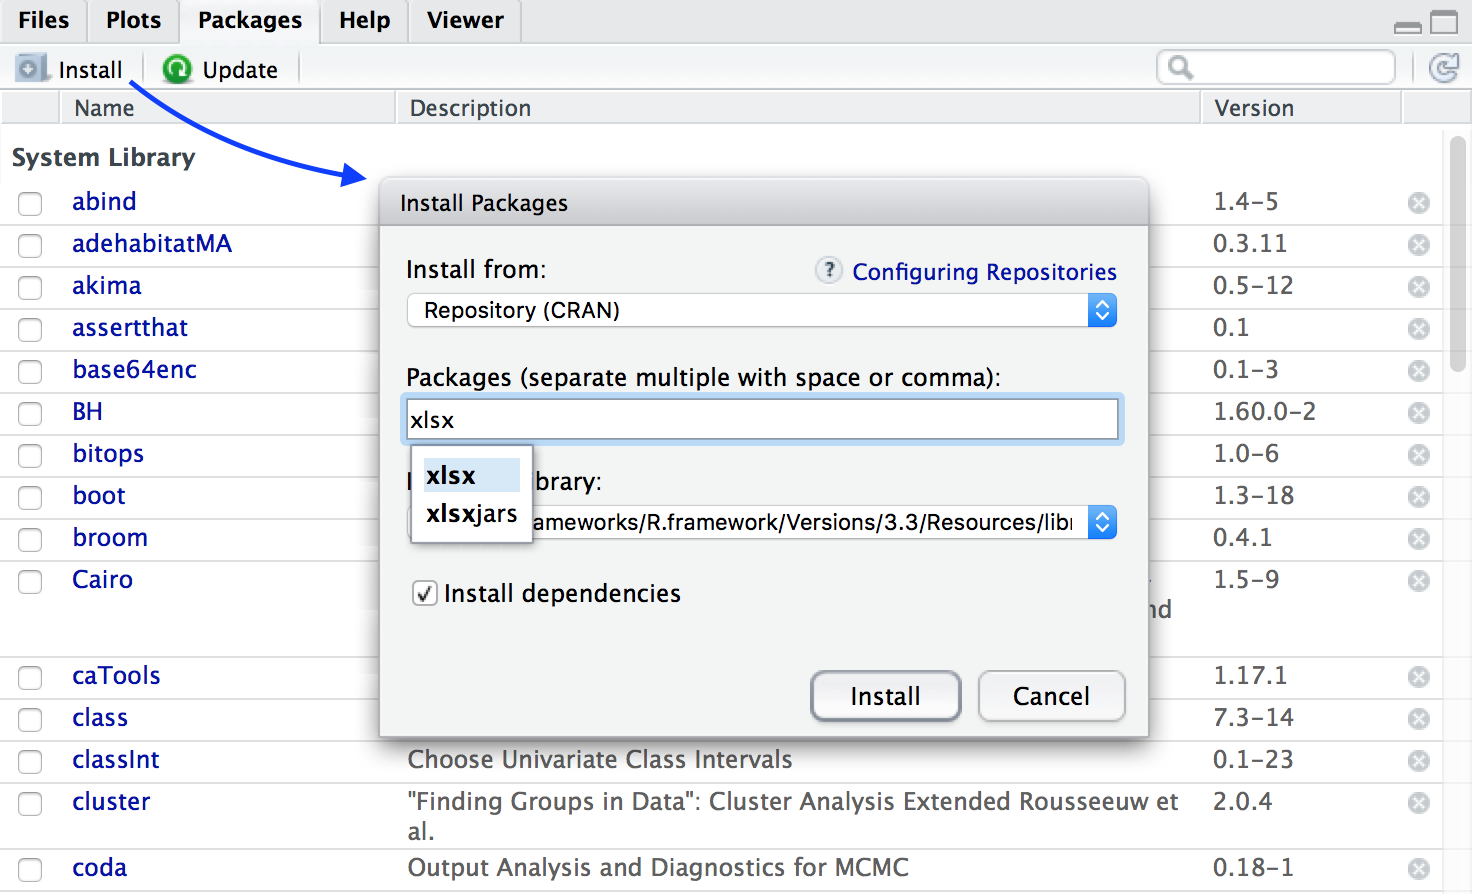
\includegraphics{images/InstallPackages.png}
\caption{\emph{Установка пакета}}
\end{figure}

Во-вторых, вы можете вызвать \emph{из консоли} команду
\texttt{install.packages()}, передав ей в качестве параметра название
пакета, заключенное в кавычки:

\begin{Shaded}
\begin{Highlighting}[]
\KeywordTok{install.packages}\NormalTok{(}\StringTok{"openxlsx"}\NormalTok{)}
\end{Highlighting}
\end{Shaded}

\begin{quote}
\textbf{Никогда не включайте команду \texttt{install.packages()} в тело
скрипта.} Это приведет к тому, что каждый раз при запуске программы
среда \textbf{RStudio} будет пытаться заново установить пакет, который
уже установлен. Запускайте эту функцию \emph{только из консоли}.
\end{quote}

\begin{quote}
\textbf{Если по каким-то причинам вы не можете установить пакет в
стандартную системную директорию RStudio} (например, из-за политик
безопасности, запрещающих запись в каталог \emph{Program Files} на ОС
\textbf{Windows}), то необходимо создать директорию вручную в другом
месте (куда вы имеете полный доступ) и указать ее адрес в параметре
\texttt{lib} функции \texttt{install.packages()}. Например:
\texttt{install.packages("xlsx",\ lib\ =\ "C:/Rlib/")}
\end{quote}

Подключение пакета осуществляется с помощью функции \texttt{library()},
при этом название пакета можно в кавычки не заключать:

\begin{Shaded}
\begin{Highlighting}[]
\KeywordTok{library}\NormalTok{(openxlsx)}
\end{Highlighting}
\end{Shaded}

\begin{quote}
\textbf{Если пакет установлен не в стандартный каталог}, а в другое
место --- например, в каталог \texttt{С:/Rlib/} (см. выше) --- то при
вызове функции \texttt{library()} необходимо указать местоположение
пакета в дополнительном параметре \texttt{lib.loc}:
\texttt{library(xlsx,\ lib.loc\ =\ "C:/Rlib")}
\end{quote}

\section*{Выполнение программного кода}\label{--}
\addcontentsline{toc}{section}{Выполнение программного кода}

Существует несколько способов выполнения исходного кода:

\begin{itemize}
\tightlist
\item
  \textbf{Выполнить одну строку}: поставить курсор в любую строку и
  нажать над редактором кода кнопку \emph{Run} или сочетание клавиш
  \texttt{Ctrl}+\texttt{Enter} (\texttt{Cmd}+\texttt{Enter} для OS X).
\item
  \textbf{Выполнить несколько строк}: выделить необходимые строки и
  нажать над редактором кода кнопку \emph{Run} или сочетание клавиш
  \texttt{Ctrl}+\texttt{Enter} (\texttt{Cmd}+\texttt{Enter} для OS X).
\item
  \textbf{Выполнить весь код} можно сразу тремя способами:

  \begin{itemize}
  \tightlist
  \item
    Выделить весь текст и нажать над редактором кода кнопку \emph{Run}
    или сочетание клавиш \texttt{Ctrl+Enter}
    (\texttt{Cmd}+\texttt{Enter} для OS X)
  \item
    Нажать клавиатурное сочетание
    \texttt{Ctrl}+\texttt{Alt}+\texttt{Enter}
    (\texttt{Cmd}+\texttt{Alt}+\texttt{Enter} для OS X)
  \item
    Нажать в правом верхнем углу редактора кода кнопку \emph{Source}
  \end{itemize}
\end{itemize}

\begin{quote}
\textbf{Команды \emph{Source} и
\texttt{Ctrl}+\texttt{Alt}+\texttt{Enter} могут не сработать}, если у
вас не установлена рабочая директория, или если в пути к рабочей
директории содержатся кириллические символы (не актуально для Windows
10+ и OS X, которые являются системами, основанными на кодировке
Unicode).
\end{quote}

Существует также ряд дополнительных опций выполнения кода, которые вы
можете найти в меню \emph{Code \textgreater{} Run Region}

\begin{quote}
\textbf{Выполняя код построчно, делайте это последовательно, начиная с
первой строки программы.} Одна из самых распространенных ошибок новичков
заключается в попытке выполнить некую строку, не выполнив
\emph{предыдущий код}. Нет никаких гарантий, что что-то получится, если
открыть файл, поставить курсор в произвольную строку посередине
программы и попытаться выполнить ее. Возможно, вам и повезет --- если
эта строка никак не зависит от предыдущего кода. Однако в реальных
программах такие строки составляют лишь небольшую долю от общего объема.
Как правило, в них происходит инициализация новых переменных стартовыми
значениями.
\end{quote}

\section*{Установка рабочей директории}\label{--}
\addcontentsline{toc}{section}{Установка рабочей директории}

Вы можете открывать и сохранять любые поддерживаемые файлы в \textbf{R},
указывая полный системный путь к файлу. Например, так может выглядеть
открытие и сохранение таблицы в формате \emph{CSV} на компьютере
\emph{Mac}:

\begin{Shaded}
\begin{Highlighting}[]
\NormalTok{d <-}\StringTok{ }\KeywordTok{read.csv}\NormalTok{(}\StringTok{"/Volumes/Data/GitHub/r-geo-course/data/oxr_vod.csv"}\NormalTok{)}
\KeywordTok{write.csv}\NormalTok{(d, }\StringTok{"/Volumes/Data/GitHub/r-geo-course/data/oxr_vod_copy.csv"}\NormalTok{)}
\end{Highlighting}
\end{Shaded}

Однако, если вам требуется открыть или сохранить несколько файлов (и не
только данных, но и графиков, карт и т.п.), программа будет выглядеть
громоздко. К тому же, прописывать каждый раз полный путь достаточно
утомительно и неприятно (даже путем копирования и вставки), а главное
--- может привести к ошибкам.

Чтобы облегчить работу с файлами, в \textbf{R} существует понятие
домашней директории. Домашняя директория задается для текущей сессии
\textbf{R} с помощью функции \texttt{setwd()}. После установки домашней
директории \textbf{R} будет полагать, что все открываемые и сохраняемые
файлы должны находиться в ней:

\begin{Shaded}
\begin{Highlighting}[]
\KeywordTok{setwd}\NormalTok{(}\StringTok{"/Volumes/Data/GitHub/r-geo-course/data"}\NormalTok{)}

\KeywordTok{read.csv}\NormalTok{(}\StringTok{"oxr_vod.csv"}\NormalTok{)}
\KeywordTok{write.csv}\NormalTok{(d, }\StringTok{"oxr_vod_copy.csv"}\NormalTok{)}
\end{Highlighting}
\end{Shaded}

Как видно, мы добавили дополнительную строчку кода, но сэкономили на
длине двух других строк. При увеличении количества обращений к файлам
польза домашней директории будет возрастать. При этом вы можете
открывать и сохранять файлы в поддиректориях, наддиректориях и соседних
директориях, используя синтаксис, стандартный для большинства
операционных систем:

\begin{Shaded}
\begin{Highlighting}[]
\CommentTok{# сохранить файл в поддиректорию data}
\KeywordTok{write.csv}\NormalTok{(d, }\StringTok{"data/oxr_vod_copy.csv"}\NormalTok{)}

\CommentTok{# сохранить файл в наддиректорию по отношению к текущей директории}
\KeywordTok{write.csv}\NormalTok{(d, }\StringTok{"../oxr_vod_copy.csv"}\NormalTok{)}

\CommentTok{# сохранить файл в директорию data, соседнюю по отношению к текущей директории}
\KeywordTok{write.csv}\NormalTok{(d, }\StringTok{"../data/oxr_vod_copy.csv"}\NormalTok{)}
\end{Highlighting}
\end{Shaded}

\begin{quote}
\textbf{Если вы перенесли код и данные с другого компьютера} (возможно,
вы получили их от своего коллеги или скачали с репозитория данного
пособия), необходимо заменить путь, указанный в функции \texttt{setwd()}
на путь к каталогу, в который вы положили данные.
\end{quote}

\begin{quote}
\textbf{Рабочая директория и местоположение скрипта могут не совпадать}.
Вы можете хранить их в разных местах. Однако рекомендуется держать их
вместе, что облегчит передачу вашей программы вместе с данными другим
пользователям.
\end{quote}

К сожалению, не существует надежного программного способа сказать среде
выполнения \textbf{R}, что в качестве домашей директории следует
использовать директорию в которой лежит сам скрипт (что, вообще говоря,
было бы крайне удобно). Возможно, в будущем разработчики языка добавят
такую полезную функцию. Однако, если для работы с \textbf{R} вы
пользуетесь средой \textbf{RStudio}, задача может быть решена путем
использования проектов. Подробнее читайте
\href{https://support.rstudio.com/hc/en-us/articles/200526207-Using-Projects}{здесь}.

\section*{Диагностические функции}\label{-}
\addcontentsline{toc}{section}{Диагностические функции}

В \textbf{R} существует ряд диагностических функций, которые позволяют
узнавать информацию об объектах, переменных, а также текущих параметрах
среды, оказывающих влияние на результаты выполнения программы. Эти
функции полезны, когда необходимо понять, какого типа, размера и
содержания данные хранятся в той или иной переменной. Нижеприведенный
список функций не являются исчерпывающим, но охватывает наиболее
употребильные функции:

\begin{longtable}[]{@{}ll@{}}
\toprule
Функция & Назначение\tabularnewline
\midrule
\endhead
\texttt{class()} & Класс (тип данных или структура данных)
объекта\tabularnewline
\texttt{str()} & Компактное представление внутренней структуры
объекта.\tabularnewline
\texttt{names()} & Названия элементов объекта\tabularnewline
\texttt{colnames()} & Названия колонок фрейма данных или
матрицы\tabularnewline
\texttt{rownames()} & Названия строк фрейма данных или
матрицы\tabularnewline
\texttt{mode()} & Режим хранения объекта.\tabularnewline
\texttt{length()} & Размер (длина) объекта.\tabularnewline
\texttt{dim()} & Измерение объекта.\tabularnewline
\texttt{sessionInfo()} & Информация о текущей сессии R и подключенных
пакетах.\tabularnewline
\texttt{options()} & Получение и установка параметров
среды.\tabularnewline
\texttt{getwd()} & Текущая рабочая директория\tabularnewline
\bottomrule
\end{longtable}

\section*{Получение справки}\label{-}
\addcontentsline{toc}{section}{Получение справки}

Любая функция \textbf{R} содержит документированное описание ее
параметров и правил использования. Справку можно получить несколькими
способами:

\begin{itemize}
\tightlist
\item
  Найти интересующую вас функцию вручную на вкладке \textbf{Packages},
  выбрав нужный пакет
\item
  Воспользоваться строкой поиска на вкладке \textbf{Help}
\item
  Ввести знак вопроса и название функции в консоли (будет искать только
  среди подключенных в настоящий момент пакетов):
\end{itemize}

\begin{Shaded}
\begin{Highlighting}[]
\KeywordTok{library}\NormalTok{(openxlsx)}

\NormalTok{?read.xlsx }\CommentTok{# равносильно вызову функции help(read.xlsx)}
\end{Highlighting}
\end{Shaded}

\begin{figure}
\centering
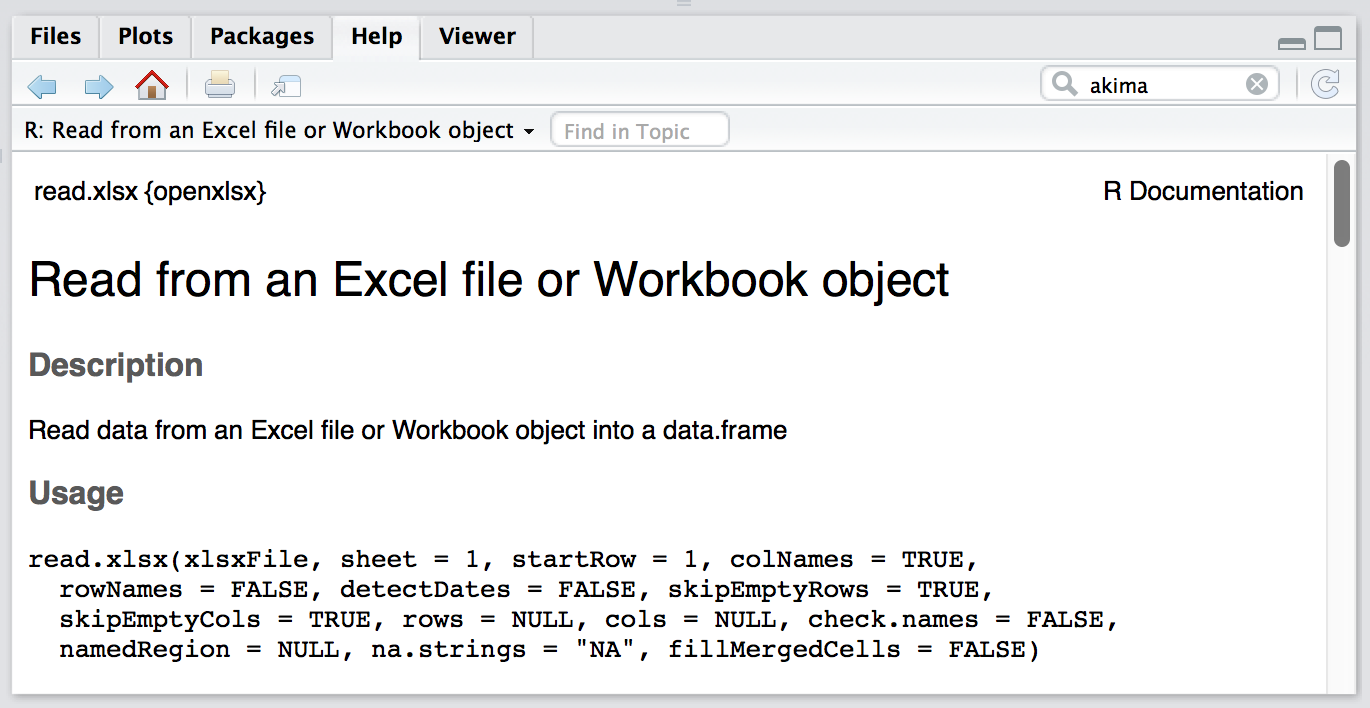
\includegraphics{images/ch0_openxlsx.png}
\caption{Справка по функции}
\end{figure}

\begin{itemize}
\tightlist
\item
  Ввести двойной знак вопроса и название функции в консоли (будет искать
  по всем установленным пакетам, независимо от того, подключены ли они в
  настоящий момент):
\end{itemize}

\begin{Shaded}
\begin{Highlighting}[]
\NormalTok{??spsample}
\end{Highlighting}
\end{Shaded}

\begin{figure}
\centering
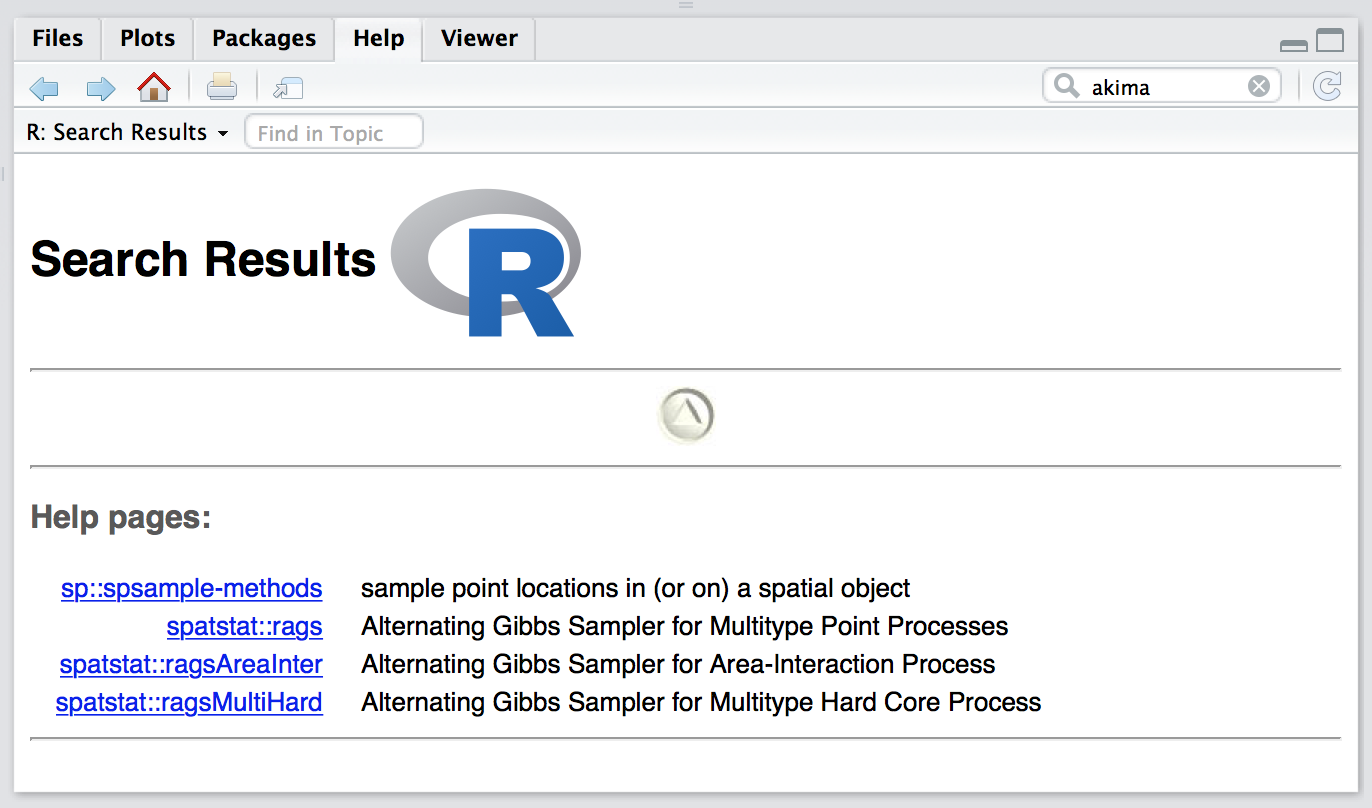
\includegraphics{images/ch0_spsample.png}
\caption{Поиск по функциям}
\end{figure}

Во многих пакетах есть также подробная документация с примерами
использования функций в виде руководств и так называемых \emph{виньеток}
(\emph{vignettes}), которые представляют из себя расширенные руководства
(статьи) по использованию пакета. С документацией пакета можно
ознакомиться, щелкнув на его названии на вкладке \emph{Packages} и
перейдя по ссылке \emph{User guides, package vignettes and other
documentation}:

\begin{figure}
\centering
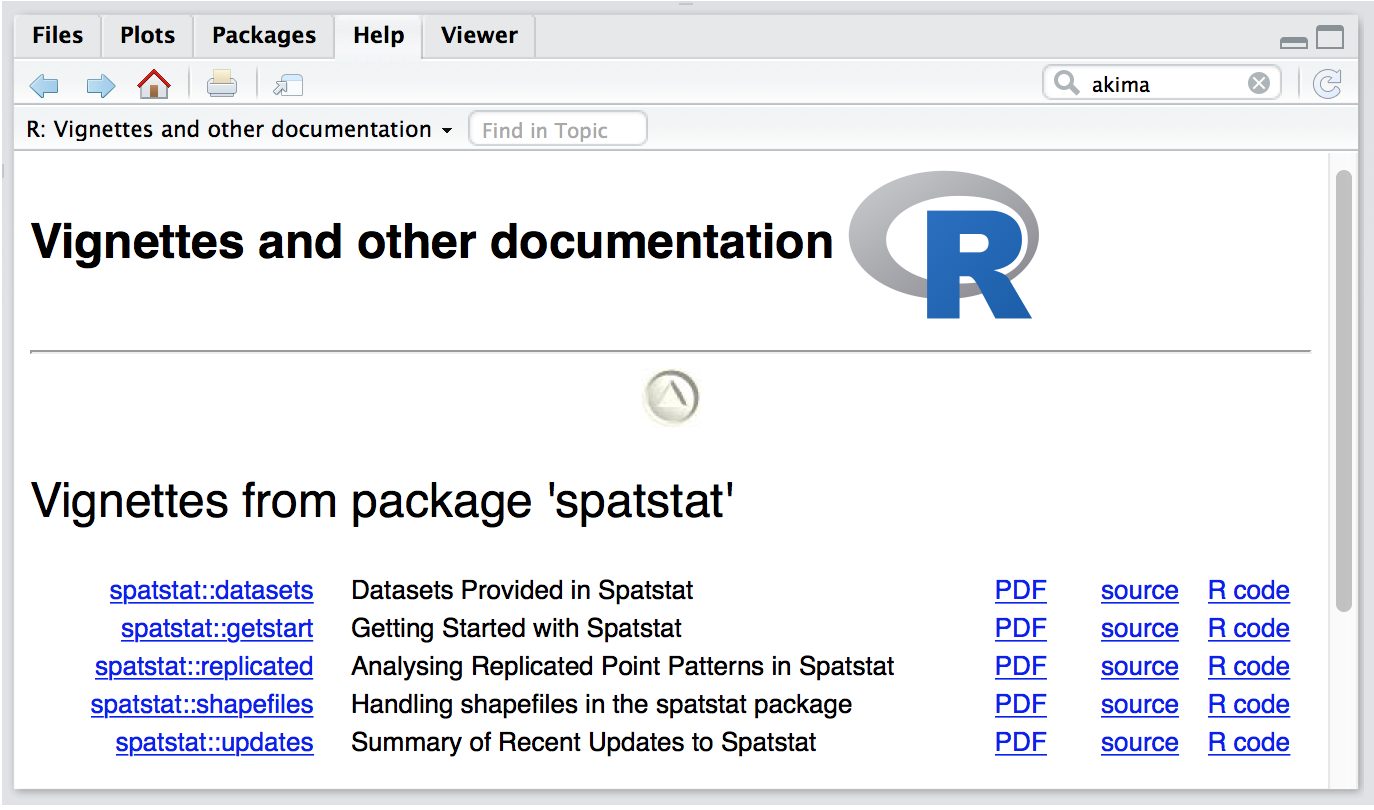
\includegraphics{images/ch0_vignette.png}
\caption{Документация пакета}
\end{figure}

\section*{Стандарт оформления кода на R}\label{----r}
\addcontentsline{toc}{section}{Стандарт оформления кода на R}

Очень важно сразу же приучить себя грамотно, структурированно и красиво
оформлять код на языке \textbf{R}. Это существенно облегчит чтение и
понимание ваших программ не только вами, но и другими пользователями и
разработчиками. Помимо вышеуказанных рекомендаций по написанию
комментариев существует также определенное количество хорошо
зарекомендовавших себя и широко используемых практик оформления кода.
Эти практики есть в каждом языке программирования и их можно найти в
литературе (и в Интернете) в виде негласных сводов правил (\emph{style
guides})

Если вы не хотите быть белой вороной в мире \textbf{R}, вам будет
полезно внимательно ознакомиться со
\href{https://google.github.io/styleguide/Rguide.xml\#filenames}{стандартом
оформления кода на R от компании Google}, которая широко использует этот
язык в своей работе.

\begin{quote}
\textbf{Стандарт оформления кода иногда также называют \emph{стилем
программирования}.} Мы не будем использовать этот термин, поскольку под
стилем программирования традиционно понимают фундаментальный подход
(\emph{парадигму}) к построению программ: процедурный, функциональный,
логический, объектно-ориентированный стиль и некоторые
\href{https://ru.wikipedia.org/wiki/Парадигма_программирования}{другие}.
\end{quote}

К числу негласных правил оформления кода на \textbf{R} можно отнести
следующие:

\begin{enumerate}
\def\labelenumi{\arabic{enumi}.}
\tightlist
\item
  Последовательно используйте знак присвоения \texttt{\textless{}-} или
  \texttt{=} на протяжении всей программы. Если вы начали использовать
  \texttt{=} -- применяйте его на протяжении всей программы, не
  используя \texttt{\textless{}-}.
\end{enumerate}

\begin{quote}
\textbf{Традиционный подход предполагает использование
\texttt{\textless{}-}}, однако все больше программистов использует знак
\texttt{=} в своих программах, что делает \textbf{R} более похожим на
другие языки программирования. Помните, что использование \texttt{=}
официально не рекомендуется, поскольку существует много старого кода на
R, который может ошибочно выполняться в сочетании с кодом, использующим
\texttt{=}. Но вы, скорее всего, с такими проблемами не столкнетесь. Так
что выбор за вами!
\end{quote}

\begin{enumerate}
\def\labelenumi{\arabic{enumi}.}
\setcounter{enumi}{1}
\tightlist
\item
  После запятой всегда ставьте пробел, перед запятой -- нет:
\end{enumerate}

\begin{Shaded}
\begin{Highlighting}[]
\CommentTok{# Правильно:}
\NormalTok{a <-}\StringTok{ }\KeywordTok{c}\NormalTok{(}\DecValTok{1}\NormalTok{, }\DecValTok{2}\NormalTok{, }\DecValTok{3}\NormalTok{, }\DecValTok{4}\NormalTok{)}
\NormalTok{m <-}\StringTok{ }\KeywordTok{matrix}\NormalTok{(a, }\DecValTok{2}\NormalTok{, }\DecValTok{2}\NormalTok{)}

\CommentTok{# Неправильно:}
\NormalTok{a <-}\StringTok{ }\KeywordTok{c}\NormalTok{(}\DecValTok{1}\NormalTok{,}\DecValTok{2}\NormalTok{,}\DecValTok{3}\NormalTok{,}\DecValTok{4}\NormalTok{)}
\NormalTok{a <-}\StringTok{ }\KeywordTok{c}\NormalTok{(}\DecValTok{1}\NormalTok{ ,}\DecValTok{2}\NormalTok{ ,}\DecValTok{3}\NormalTok{ ,}\DecValTok{4}\NormalTok{)}
\NormalTok{a <-}\StringTok{ }\KeywordTok{c}\NormalTok{(}\DecValTok{1}\NormalTok{ , }\DecValTok{2}\NormalTok{ , }\DecValTok{3}\NormalTok{ , }\DecValTok{4}\NormalTok{)}
\NormalTok{m <-}\StringTok{ }\KeywordTok{matrix}\NormalTok{(a,}\DecValTok{2}\NormalTok{,}\DecValTok{2}\NormalTok{)}
\NormalTok{m <-}\StringTok{ }\KeywordTok{matrix}\NormalTok{(a ,}\DecValTok{2}\NormalTok{ ,}\DecValTok{2}\NormalTok{)}
\NormalTok{m <-}\StringTok{ }\KeywordTok{matrix}\NormalTok{(a , }\DecValTok{2}\NormalTok{ , }\DecValTok{2}\NormalTok{)}
\end{Highlighting}
\end{Shaded}

\begin{enumerate}
\def\labelenumi{\arabic{enumi}.}
\setcounter{enumi}{2}
\tightlist
\item
  Отделяйте любые бинарные операторы (такие как
  \texttt{=,\ +,\ -,\ \textless{}-,\ *}) пробелами с двух сторон:
\end{enumerate}

\begin{Shaded}
\begin{Highlighting}[]
\NormalTok{a <-}\StringTok{ }\KeywordTok{sin}\NormalTok{(b }\OperatorTok{+}\StringTok{ }\NormalTok{pi }\OperatorTok{*}\StringTok{ }\FloatTok{0.5}\NormalTok{) }\CommentTok{# правильно}
\NormalTok{a<-}\KeywordTok{sin}\NormalTok{(b}\OperatorTok{+}\NormalTok{pi}\OperatorTok{*}\FloatTok{0.5}\NormalTok{) }\CommentTok{# неправильно}
\end{Highlighting}
\end{Shaded}

\begin{enumerate}
\def\labelenumi{\arabic{enumi}.}
\setcounter{enumi}{3}
\tightlist
\item
  Между названием функции и открывающей скобкой пробела быть не должно.
  То же самое касается обращения к элементам вектора, матрицы и т.п.:
\end{enumerate}

\begin{Shaded}
\begin{Highlighting}[]
\CommentTok{# Правильно:}
\KeywordTok{sin}\NormalTok{(b)}
\NormalTok{a[}\DecValTok{2}\NormalTok{]}

\CommentTok{# Неправильно:}
\KeywordTok{sin}\NormalTok{ (b)}
\NormalTok{a [}\DecValTok{2}\NormalTok{]}
\end{Highlighting}
\end{Shaded}

\begin{enumerate}
\def\labelenumi{\arabic{enumi}.}
\setcounter{enumi}{4}
\tightlist
\item
  В то же время, при вызове команд управления выполнением программы
  (условные операторы и циклы) перед и после скобок пробел
  \textbf{должен} стоять:
\end{enumerate}

\begin{Shaded}
\begin{Highlighting}[]
\CommentTok{# Правильно:}
\ControlFlowTok{if}\NormalTok{ (a }\OperatorTok{>}\StringTok{ }\DecValTok{0}\NormalTok{) \{}
  \KeywordTok{print}\NormalTok{(a)}
\NormalTok{\}}
\NormalTok{i <-}\StringTok{ }\DecValTok{0}
\ControlFlowTok{while}\NormalTok{ (i }\OperatorTok{<}\StringTok{ }\NormalTok{a) \{}
  \KeywordTok{print}\NormalTok{(i)}
\NormalTok{  i <-}\StringTok{ }\NormalTok{i }\OperatorTok{+}\StringTok{ }\DecValTok{1}
\NormalTok{\}}

\CommentTok{# Неправильно:}
\ControlFlowTok{if}\NormalTok{(a }\OperatorTok{>}\StringTok{ }\DecValTok{0}\NormalTok{)\{}
  \KeywordTok{print}\NormalTok{(a)}
\NormalTok{\}}

\NormalTok{i <-}\StringTok{ }\DecValTok{0}
\ControlFlowTok{while}\NormalTok{(i }\OperatorTok{<}\StringTok{ }\NormalTok{a)\{}
  \KeywordTok{print}\NormalTok{(i)}
\NormalTok{  i <-}\StringTok{ }\NormalTok{i }\OperatorTok{+}\StringTok{ }\DecValTok{1}
\NormalTok{\}}
\end{Highlighting}
\end{Shaded}

\section*{Комментарии}
\addcontentsline{toc}{section}{Комментарии}

\textbf{Комментарии} --- это фрагменты текста программы, начинающиеся с
символа \texttt{\#}. Комментарии не воспринимаются как исполняемый код и
служат для документирования программы. При выполнении программы
содержимое комментария в зависимости от настроек среды может выводиться
или не выводиться в консоль, однако их содержание никак не влияет на
результаты выполнения программы.

\begin{quote}
\textbf{Всегда пишите комментарии}, чтобы по прошествии времени можно
было открыть файл и быстро восстановить в памяти логику программы и
смысл отдельных операций. Комментарии особенно необходимы, если вашей
программой будет пользоваться кто-то другой --- без них будет трудно
разобраться в программном коде.
\end{quote}

Действие комментария продолжается от символа \texttt{\#} до конца
строки. Соответственно, вы можете поставить данный символ в самом начале
строки и тогда комментарий будет занимать всю строку. Комментарий также
можно расположить справа от исполняемого кода, и тогда он будет занимать
только часть строки.

\begin{quote}
\textbf{Прервать комментарий и написать справа от него исполняемый код
нельзя}
\end{quote}

Полнострочные комментарии часто используются для выделения разделов в
программе и написания объемных пояснений. Часто в них вводят имитации
разделительных линий с помощью символов дефиса (\texttt{-}) или
подчеркивания (\texttt{\_}), а заголовки набирают прописными буквами.
Короткие комментарии справа от фрагментов кода обычно служат пояснением
конкретных простых операций. Подобная логика употребления комментариев
не является обязательной. Вы можете оформлять их на свое усмотрение.
Главное, чтобы они выполняли свою основную функцию --- пояснять смысл
выполняемых действий. Например:

\begin{Shaded}
\begin{Highlighting}[]
\CommentTok{# ОПЕРАЦИИ С ЧИСЛАМИ}
\CommentTok{# ---------------------------}
\CommentTok{# В данном разделе рассматриваются арифметические операции, такие как сложение, вычитание, деление, деление с остатком, взятие остатка и возведение в степень:}

\NormalTok{a <-}\StringTok{ }\DecValTok{3} \OperatorTok{+}\StringTok{ }\DecValTok{2} \CommentTok{# Сложение}
\NormalTok{b <-}\StringTok{ }\DecValTok{4} \OperatorTok{^}\StringTok{ }\DecValTok{8} \CommentTok{# Возведение в степень}
\NormalTok{c <-}\StringTok{ }\NormalTok{b }\OperatorTok\StringTok{ }\NormalTok{a }\CommentTok{# Взятие остатка}

\CommentTok{# Деление}
\NormalTok{d <-}\StringTok{ }\NormalTok{c }\OperatorTok{/}\StringTok{ }\NormalTok{a }

\CommentTok{# Умножение}
\NormalTok{e <-}\StringTok{ }\NormalTok{d }\OperatorTok{*}\StringTok{ }\NormalTok{b}
\end{Highlighting}
\end{Shaded}

Однако, усердствовать с комментированием каждой мелочи в программе,
разумеется, не стоит. Со временем у вас выработается взвешенный подход к
документированию программ и понимание того, какие ее фрагменты требуют
пояснения, а какие самоочевидны.

\begin{quote}
\textbf{Для быстрой вставки комментария, обозначающего новый раздел
программы}, воспользуйтесь командой меню \emph{Code \textgreater{}
Insert Section} или клавиатурным сочетанием
\texttt{Ctrl}+\texttt{Shift}+\texttt{R}
(\texttt{Cmd}+\texttt{Shift}+\texttt{R} для OS X)
\end{quote}

\section*{Названия специальных символов}\label{--}
\addcontentsline{toc}{section}{Названия специальных символов}

В \textbf{R}, как и во многих других языках программирования испльзуются
различные специальные символы. Их смысл и значение мы узнаем по ходу
изучения языка, а пока что выучите их названия, чтобы грамотно
употреблять в своей речи

\begin{longtable}[]{@{}ll@{}}
\toprule
Символ & Название\tabularnewline
\midrule
\endhead
\texttt{\$} & доллар\tabularnewline
\texttt{\#} & шарп\tabularnewline
\texttt{\&} & амперсанд (решетка)\tabularnewline
\texttt{/} & прямой слэш\tabularnewline
\texttt{\textbackslash{}} & обратный слэш\tabularnewline
\texttt{\textbar{}} & пайп (вертикальная черта)\tabularnewline
\texttt{\^{}} & циркумфлекс (крышечка)\tabularnewline
\texttt{@} & эт (собачка)\tabularnewline
\texttt{\textasciitilde{}} & тильда\tabularnewline
\texttt{\textquotesingle{}\textquotesingle{}} & одинарные
кавычки\tabularnewline
\texttt{""} & двойные кавычки\tabularnewline
\texttt{\textasciigrave{}\textasciigrave{}} & обратные
кавычки\tabularnewline
\bottomrule
\end{longtable}

\section*{Ссылка на пособие}\label{--}
\addcontentsline{toc}{section}{Ссылка на пособие}

Если этот курс лекций оказался полезным для вас, и вы хотите
процитировать его с списке литературы вашей работы, то ссылку можно
оформить по следующей форме:

\begin{longtable}[]{@{}l@{}}
\toprule
\emph{Самсонов Т.Е.} \textbf{Визуализация и анализ географических данных
на языке R.} М.: Географический факультет МГУ, 2017. DOI:
10.5281/zenodo.901911\tabularnewline
\bottomrule
\end{longtable}

\chapter{Типы данных. Ввод и вывод}\label{data_types}

Тип данных --- это класс данных, характеризуемый членами класса и
операциями, которые могут быть к ним применены\footnote{ISO/IEC/IEEE
  24765-2010 Systems and software engineering --- Vocabulary}. С помощью
типов данных мы можем представлять привычные нам сущности, такие как
числа, строки и т.д. В языке R существует 5 базовых типов данных:

\begin{longtable}[]{@{}ll@{}}
\toprule
Название & Тип данных\tabularnewline
\midrule
\endhead
\texttt{complex} & комплексные числа\tabularnewline
\texttt{character} & строки\tabularnewline
\texttt{integer} & целые числа\tabularnewline
\texttt{logical} & логические (булевы)\tabularnewline
\texttt{numeric} & числа с плавающей точкой\tabularnewline
\bottomrule
\end{longtable}

Помимо этого есть тип \texttt{Date}, который позволяет работать с
датами. Рассмотрим использование каждого из перечисленных типов.

\section{Числа}\label{numbers}

Числа --- основной тип данных в R. К ним относятся \emph{числа c
плавающей точкой} и \emph{целые числа}. В терминологии R такие данные
называются \emph{интервальными}, поскольку к ним применимо понятие
интервала на числовой прямой. Целые числа относятся к \emph{дискретным
интервальным}, а числа с плавающей точкой --- к \emph{непрерывным
интервальным}. Числа можно складывать, вычитать и умножать:

\begin{Shaded}
\begin{Highlighting}[]
\DecValTok{2} \OperatorTok{+}\StringTok{ }\DecValTok{3}
\NormalTok{## [1] 5}
\DecValTok{2} \OperatorTok{-}\StringTok{ }\DecValTok{3}
\NormalTok{## [1] -1}
\DecValTok{2} \OperatorTok{*}\StringTok{ }\DecValTok{3}
\NormalTok{## [1] 6}
\end{Highlighting}
\end{Shaded}

Разделителем целой и дробной части является точка, а не запятая:

\begin{Shaded}
\begin{Highlighting}[]
\FloatTok{2.5} \OperatorTok{+}\StringTok{ }\FloatTok{3.1}
\NormalTok{## [1] 5.6}
\end{Highlighting}
\end{Shaded}

Существует также специальный оператор для возведения в степень. Для
этого вы можете использовать или двойной знак умножения (\texttt{**})
или \emph{циркумфлекс} (\texttt{\^{}}), который в обиходе называют
просто ``крышечкой'':

\begin{Shaded}
\begin{Highlighting}[]
\DecValTok{2} \OperatorTok{^}\StringTok{ }\DecValTok{3}
\NormalTok{## [1] 8}
\DecValTok{2} \OperatorTok{**}\StringTok{ }\DecValTok{3}
\NormalTok{## [1] 8}
\end{Highlighting}
\end{Shaded}

Результат деления по умолчанию имеет тип с плавающей точкой:

\begin{Shaded}
\begin{Highlighting}[]
\DecValTok{5} \OperatorTok{/}\StringTok{ }\DecValTok{3}
\NormalTok{## [1] 1.666667}
\DecValTok{5} \OperatorTok{/}\StringTok{ }\FloatTok{2.5}
\NormalTok{## [1] 2}
\end{Highlighting}
\end{Shaded}

Если вы хотите чтобы деление производилось целочисленным образом (без
дробной части) необходимо использовать оператор \texttt{\%/\%}:

\begin{Shaded}
\begin{Highlighting}[]
\DecValTok{5} \OperatorTok\StringTok{ }\DecValTok{3}
\NormalTok{## [1] 1}
\end{Highlighting}
\end{Shaded}

Остаток от деления можно получить с помощью оператора \texttt{\%\%}:

\begin{Shaded}
\begin{Highlighting}[]
\DecValTok{5} \OperatorTok\StringTok{ }\DecValTok{3}
\NormalTok{## [1] 2}
\end{Highlighting}
\end{Shaded}

Вышеприведенные арифметические операции являются бинарными, то есть
требуют наличия двух чисел. Числа называются ``операндами''. Отделять
операнды от оператора пробелом или нет --- дело вкуса. Я предпочитаю
отделять, так как это повышает читаемость кода. Следующие два выражения
эквивалентны. Однако сравните простоту их восприятия:

\begin{Shaded}
\begin{Highlighting}[]
\DecValTok{5}\OperatorTok\DecValTok{3}
\NormalTok{## [1] 1}
\end{Highlighting}
\end{Shaded}

\begin{Shaded}
\begin{Highlighting}[]
\DecValTok{5} \OperatorTok\StringTok{ }\DecValTok{3}
\NormalTok{## [1] 1}
\end{Highlighting}
\end{Shaded}

Как правило, в настоящих программах числа в явном виде встречаются лишь
иногда. Вместо этого для их обозначения используют переменные. В
вышеприведенных выражениях мы неоднократно использовали число 3. Теперь
представьте, что вы хотите проверить, каковы будут результаты, если
вместо 3 использовать 4. Вам придется заменить все тройки на четверки.
Если их много, то это будет утомительная работа, и вы наверняка что-то
пропустите. Конечно, можно использовать поиск с автозаменой, но что если
тройки надо заменить не везде? Одно и то же число может выполнять разные
функции в разных выражениях. Чтобы избежать подобных проблем, в
программе вводят переменные и присваивают им значения. Оператор
присваивания значения выглядит как \texttt{\textless{}-}

\begin{Shaded}
\begin{Highlighting}[]
\NormalTok{a <-}\StringTok{ }\DecValTok{5}
\NormalTok{b <-}\StringTok{ }\DecValTok{3}
\end{Highlighting}
\end{Shaded}

Чтобы вывести значение переменной на экран, достаточно просто ввести
его:

\begin{Shaded}
\begin{Highlighting}[]
\NormalTok{a}
\NormalTok{## [1] 5}
\NormalTok{b}
\NormalTok{## [1] 3}
\end{Highlighting}
\end{Shaded}

Мы можем выполнить над переменными все те же операции что и над
константами:

\begin{Shaded}
\begin{Highlighting}[]
\NormalTok{a }\OperatorTok{+}\StringTok{ }\NormalTok{b}
\NormalTok{## [1] 8}
\NormalTok{a }\OperatorTok{-}\StringTok{ }\NormalTok{b}
\NormalTok{## [1] 2}
\NormalTok{a }\OperatorTok{/}\StringTok{ }\NormalTok{b}
\NormalTok{## [1] 1.666667}
\NormalTok{a }\OperatorTok\StringTok{ }\NormalTok{b}
\NormalTok{## [1] 1}
\NormalTok{a }\OperatorTok\StringTok{ }\NormalTok{b}
\NormalTok{## [1] 2}
\end{Highlighting}
\end{Shaded}

Легко меняем значение второй переменной с 3 на 4 и выполняем код заново.

\begin{Shaded}
\begin{Highlighting}[]
\NormalTok{b <-}\StringTok{ }\DecValTok{4}
\NormalTok{a }\OperatorTok{+}\StringTok{ }\NormalTok{b}
\NormalTok{## [1] 9}
\NormalTok{a }\OperatorTok{-}\StringTok{ }\NormalTok{b}
\NormalTok{## [1] 1}
\NormalTok{a }\OperatorTok{/}\StringTok{ }\NormalTok{b}
\NormalTok{## [1] 1.25}
\NormalTok{a }\OperatorTok\StringTok{ }\NormalTok{b}
\NormalTok{## [1] 1}
\NormalTok{a }\OperatorTok\StringTok{ }\NormalTok{b}
\NormalTok{## [1] 1}
\end{Highlighting}
\end{Shaded}

Нам пришлось изменить значение переменной только один раз в момент ее
создания, все последующие операции остались неизменны, но их результаты
обновились!

Новую переменную можно создать на основе значений существующих
переменных:

\begin{Shaded}
\begin{Highlighting}[]
\NormalTok{c <-}\StringTok{ }\NormalTok{b}
\NormalTok{d <-}\StringTok{ }\NormalTok{a}\OperatorTok{+}\NormalTok{c}
\end{Highlighting}
\end{Shaded}

Посмотрим, что получилось:

\begin{Shaded}
\begin{Highlighting}[]
\NormalTok{c}
\NormalTok{## [1] 4}
\NormalTok{d}
\NormalTok{## [1] 9}
\end{Highlighting}
\end{Shaded}

Вы можете комбинировать переменные и заданные явным образом константы:

\begin{Shaded}
\begin{Highlighting}[]
\NormalTok{e <-}\StringTok{ }\NormalTok{d }\OperatorTok{+}\StringTok{ }\FloatTok{2.5}
\NormalTok{e}
\NormalTok{## [1] 11.5}
\end{Highlighting}
\end{Shaded}

Противоположное по знаку число получается добавлением унарного оператора
\texttt{-} перед константой или переменной:

\begin{Shaded}
\begin{Highlighting}[]
\NormalTok{f <-}\StringTok{ }\OperatorTok{-}\DecValTok{2}
\NormalTok{f}
\NormalTok{## [1] -2}
\NormalTok{f <-}\StringTok{ }\OperatorTok{-}\NormalTok{e}
\NormalTok{f}
\NormalTok{## [1] -11.5}
\end{Highlighting}
\end{Shaded}

Операция взятия остатка от деления бывает полезной, например, когда мы
хотим выяснить, является число четным или нет. Для этого достаточно
взять остаток от деления на 2. Если число является четным, остаток будет
равен нулю. В данном случае c равно 4, \texttt{d} равно 9:

\begin{Shaded}
\begin{Highlighting}[]
\NormalTok{c }\OperatorTok\StringTok{ }\DecValTok{2}
\NormalTok{## [1] 0}
\NormalTok{d }\OperatorTok\StringTok{ }\DecValTok{2}
\NormalTok{## [1] 1}
\end{Highlighting}
\end{Shaded}

\subsection{Числовые функции}\label{number_functions}

Прежде чем мы перейдем к рассмотрению прочих типов данных и структур
данных нам необходимо познакомиться с функциями, поскольку они
встречаются буквально на каждом шагу. Понятие функции идентично тому, к
чему мы привыкли в математике. Например, функция может называться
\texttt{Z}, и принимать 2 аргумента: \texttt{x} и \texttt{y}. В этом
случае она записывается как \texttt{Z(x,y)}. Чтобы получить значение
функции, необходимо подставить некоторые значения вместо \texttt{x} и
\texttt{y} в скобках. Нас даже может не интересовать, как фактически
устроена функция внутри, но важно понимать, что именно она должна
вычислять. С созданием функций мы познакомимся позднее.

Важнейшие примеры функций --- математические. Это функции взятия корня
\texttt{sqrt(x)}, модуля \texttt{abs(x)}, округления
\texttt{round(x,\ digits)}, натурального логарифма \texttt{abs(x)},
тригонометрические функции \texttt{sin(x)}, \texttt{cos(x)},
\texttt{tan(x)}, обратные к ним \texttt{asin(y)}, \texttt{acos(y)},
\texttt{atan(y)} и многие другие. Основные математические функции
содержатся в пакете
\href{https://stat.ethz.ch/R-manual/R-devel/library/base/html/00Index.html}{\texttt{base}},
который по умолчанию доступен в среде R и не требует подключения.

В качестве аргумента функции можно использовать переменную, константу, а
также выражения:

\begin{Shaded}
\begin{Highlighting}[]
\KeywordTok{sqrt}\NormalTok{(a)}
\NormalTok{## [1] 2.236068}
\KeywordTok{sin}\NormalTok{(a)}
\NormalTok{## [1] -0.9589243}
\KeywordTok{tan}\NormalTok{(}\FloatTok{1.5}\NormalTok{)}
\NormalTok{## [1] 14.10142}
\KeywordTok{abs}\NormalTok{(a }\OperatorTok{+}\StringTok{ }\NormalTok{b }\OperatorTok{-}\StringTok{ }\FloatTok{2.5}\NormalTok{)}
\NormalTok{## [1] 6.5}
\end{Highlighting}
\end{Shaded}

Вы также можете легко вкладывать функции одна в одну, если результат
вычисления одной функции нужно подставить в другую:

\begin{Shaded}
\begin{Highlighting}[]
\KeywordTok{sin}\NormalTok{(}\KeywordTok{sqrt}\NormalTok{(a))}
\NormalTok{## [1] 0.7867491}
\KeywordTok{sqrt}\NormalTok{(}\KeywordTok{sin}\NormalTok{(a) }\OperatorTok{+}\StringTok{ }\DecValTok{2}\NormalTok{)}
\NormalTok{## [1] 1.020331}
\end{Highlighting}
\end{Shaded}

Также как и с арифметическими выражениями, результат вычисления функции
можно записать в переменную:

\begin{Shaded}
\begin{Highlighting}[]
\NormalTok{b <-}\StringTok{ }\KeywordTok{sin}\NormalTok{(}\KeywordTok{sqrt}\NormalTok{(a))}
\NormalTok{b}
\NormalTok{## [1] 0.7867491}
\end{Highlighting}
\end{Shaded}

Если переменной b ранее было присвоено другое значение, оно
перезапишется. Вы также можете записать в переменную результат операции,
выполненной над ней же. Например, если вы не уверены, что \texttt{a} ---
неотрицательное число, а вам это необходимо в дальнейших расчетах, вы
можете применить к нему операцию взятия модуля:

\begin{Shaded}
\begin{Highlighting}[]
\NormalTok{b <-}\StringTok{ }\KeywordTok{sin}\NormalTok{(a)}
\NormalTok{b}
\NormalTok{## [1] -0.9589243}
\NormalTok{b <-}\StringTok{ }\KeywordTok{abs}\NormalTok{(b)}
\NormalTok{b}
\NormalTok{## [1] 0.9589243}
\end{Highlighting}
\end{Shaded}

\section{Строки}\label{strings}

Строки --- также еще один важнейший тип данных. Строки состоят из
символов. Чтобы создать строковую переменную, необходимо заключить текст
строки в кавычки:

\begin{Shaded}
\begin{Highlighting}[]
\NormalTok{s <-}\StringTok{ "В историю трудно войти, но легко вляпаться (М.Жванецкий)"}
\NormalTok{s}
\NormalTok{## [1] "В историю трудно войти, но легко вляпаться (М.Жванецкий)"}
\end{Highlighting}
\end{Shaded}

Длину строки в символах можно узнать с помощью функции \texttt{nchar()}

\begin{Shaded}
\begin{Highlighting}[]
\KeywordTok{nchar}\NormalTok{(s)}
\NormalTok{## [1] 56}
\end{Highlighting}
\end{Shaded}

Строки можно складывать так же как и числа. Эта операция называется
\emph{конкатенацией}. В результате конкатенации строки состыковываются
друг с другом и получается одна строка. В отличие от чисел, конкатенация
производится не оператором \texttt{+}, а специальной функцией
\texttt{paste()}. Состыковываемые строки нужно перечислить через
запятую, их число может быть произвольно

\begin{Shaded}
\begin{Highlighting}[]
\NormalTok{s1 <-}\StringTok{ "В историю трудно войти,"}
\NormalTok{s2 <-}\StringTok{ "но легко вляпаться"}
\NormalTok{s3 <-}\StringTok{ "(М.Жванецкий)"}
\end{Highlighting}
\end{Shaded}

Посмотрим содержимое подстрок:

\begin{Shaded}
\begin{Highlighting}[]
\NormalTok{s1}
\NormalTok{## [1] "В историю трудно войти,"}
\NormalTok{s2}
\NormalTok{## [1] "но легко вляпаться"}
\NormalTok{s3}
\NormalTok{## [1] "(М.Жванецкий)"}
\end{Highlighting}
\end{Shaded}

А теперь объединим их в одну:

\begin{Shaded}
\begin{Highlighting}[]
\NormalTok{s <-}\StringTok{ }\KeywordTok{paste}\NormalTok{(s1, s2)}
\NormalTok{s}
\NormalTok{## [1] "В историю трудно войти, но легко вляпаться"}
\NormalTok{s <-}\StringTok{ }\KeywordTok{paste}\NormalTok{(s1, s2, s3)}
\NormalTok{s}
\NormalTok{## [1] "В историю трудно войти, но легко вляпаться (М.Жванецкий)"}
\end{Highlighting}
\end{Shaded}

Настоящая сила конкатенации проявляется когда вам необходимо объединить
в одной строке некоторое текстовое описание (заранее известное) и
значения переменных, которые у вас вычисляются в программе (заранее
неизвестные). Предположим, вы нашли в программе что максимальная
численность населения в Детройте пришлась на 1950 год и составила 1850
тыс. человек. Найденный год записан у вас в переменную \texttt{year}, а
население в переменную \texttt{pop}. Вы их значения пока что не знаете,
они вычислены по табличным данным в программе. Как вывести эту
информацию на экран ``человеческим''" образом? Для этого нужно
использовать конкатенацию строк.

Условно запишем значения переменных, как будто мы их знаем

\begin{Shaded}
\begin{Highlighting}[]
\NormalTok{year <-}\StringTok{ }\DecValTok{1950}
\NormalTok{pop <-}\StringTok{ }\DecValTok{1850}
\end{Highlighting}
\end{Shaded}

\begin{Shaded}
\begin{Highlighting}[]
\NormalTok{s1 <-}\StringTok{ "Максимальная численность населения в Детройте пришлась на"}
\NormalTok{s2 <-}\StringTok{ "год и составила"}
\NormalTok{s3 <-}\StringTok{ "тыс. чел"}
\NormalTok{s <-}\StringTok{ }\KeywordTok{paste}\NormalTok{(s1, year, s2, pop, s3)}
\NormalTok{s}
\NormalTok{## [1] "Максимальная численность населения в Детройте пришлась на 1950 год и составила 1850 тыс. чел"}
\end{Highlighting}
\end{Shaded}

Обратите внимание на то что мы конкатенировали строки с числами.
Конвертация типов осуществилась автоматически. Помимо этого, функция
сама вставила пробелы между строками.

\section{Даты}\label{dates}

Даты являются необходимыми при работе с временными данными. В
географическом анализе подобные задачи возникают сплошь и рядом.
Точность указания времени может быть самой различной. От года до долей
секунды. Чаще всего используются даты, указанные с точностью до дня. Для
создания даты используется функция \texttt{as.Date()}. В данном случае
точка --- это лишь часть названия функции, а не какой-то особый
оператор. В качестве аргумента функции необходимо задать дату,
записанную в виде строки. Запишем дату рождения автора (можете заменить
ее на свою):

\begin{Shaded}
\begin{Highlighting}[]
\NormalTok{birth <-}\StringTok{ }\KeywordTok{as.Date}\NormalTok{(}\StringTok{'1986/02/18'}\NormalTok{)}
\NormalTok{birth}
\NormalTok{## [1] "1986-02-18"}
\end{Highlighting}
\end{Shaded}

Сегодняшнюю дату вы можете узнать с помощью специальной функции
\texttt{Sys.Date()}:

\begin{Shaded}
\begin{Highlighting}[]
\NormalTok{current <-}\StringTok{ }\KeywordTok{Sys.Date}\NormalTok{()}
\NormalTok{current}
\NormalTok{## [1] "2017-10-05"}
\end{Highlighting}
\end{Shaded}

Даты также можно складывать и вычитать. В зависимости от дискретности
данных, вы получите результат в часах, днях, годах и т.д. Например,
узнать продолжительность жизни в днях можно так:

\begin{Shaded}
\begin{Highlighting}[]
\NormalTok{livedays <-}\StringTok{ }\NormalTok{current }\OperatorTok{-}\StringTok{ }\NormalTok{birth}
\NormalTok{livedays}
\NormalTok{## Time difference of 11552 days}
\end{Highlighting}
\end{Shaded}

Вы также можете прибавить к текущей дате некоторое значение. Например,
необходимо узнать, какая дата будет через 40 дней:

\begin{Shaded}
\begin{Highlighting}[]
\NormalTok{current }\OperatorTok{+}\StringTok{ }\DecValTok{40}
\NormalTok{## [1] "2017-11-14"}
\end{Highlighting}
\end{Shaded}

\section{Логические}\label{booleans}

Логические переменные возникают там, где нужно проверить условие.
Переменная логического типа может принимать значение \texttt{TRUE}
(истина) или \texttt{FALSE} (ложь). Для их обозначения также возможны
более компактные константы \texttt{T} и \texttt{F} соответственно.

Следующие операторы приводят к возникновению логических переменных:

\begin{itemize}
\tightlist
\item
  \emph{РАВНО} (\texttt{==}) --- проверка равенства операндов
\item
  \emph{НЕ РАВНО} (\texttt{!=}) --- проверка неравенства операндов
\item
  \emph{МЕНЬШЕ} (\texttt{\textless{}}) --- первый аргумент меньше
  второго
\item
  \emph{МЕНЬШЕ ИЛИ РАВНО} (\texttt{\textless{}=}) --- первый аргумент
  меньше или равен второму
\item
  \emph{БОЛЬШЕ} (\texttt{\textgreater{}}) --- первый аргумент больше
  второго
\item
  \emph{БОЛЬШЕ ИЛИ РАВНО} (\texttt{\textgreater{}=}) --- первый аргумент
  больше или равен второму
\end{itemize}

Посмотрим, как они работают:

\begin{Shaded}
\begin{Highlighting}[]
\NormalTok{a <-}\StringTok{ }\DecValTok{1}
\NormalTok{b <-}\StringTok{ }\DecValTok{2}
\NormalTok{a }\OperatorTok{==}\StringTok{ }\NormalTok{b}
\NormalTok{## [1] FALSE}
\NormalTok{a }\OperatorTok{!=}\StringTok{ }\NormalTok{b}
\NormalTok{## [1] TRUE}
\NormalTok{a }\OperatorTok{>}\StringTok{ }\NormalTok{b}
\NormalTok{## [1] FALSE}
\NormalTok{a }\OperatorTok{<}\StringTok{ }\NormalTok{b}
\NormalTok{## [1] TRUE}
\end{Highlighting}
\end{Shaded}

Если необходимо проверить несколько условий одновременно, их можно
комбинировать с помощью логических операторов. Наиболее популярные среди
них:

\begin{itemize}
\tightlist
\item
  \emph{И} (\texttt{\&\&}) - проверка истинности обоих условий
\item
  \emph{ИЛИ} (\texttt{\textbar{}\textbar{}}) - проверка истинности хотя
  бы одного из условий
\item
  \emph{НЕ} (\texttt{!}) - отрицание операнда (истина меняется на ложь,
  ложь на истину)
\end{itemize}

\begin{Shaded}
\begin{Highlighting}[]
\NormalTok{c<-}\DecValTok{3}
\NormalTok{(b}\OperatorTok{>}\NormalTok{a) }\OperatorTok{&&}\StringTok{ }\NormalTok{(c}\OperatorTok{>}\NormalTok{b)}
\NormalTok{## [1] TRUE}
\NormalTok{(a}\OperatorTok{>}\NormalTok{b) }\OperatorTok{&&}\StringTok{ }\NormalTok{(c}\OperatorTok{>}\NormalTok{b)}
\NormalTok{## [1] FALSE}
\NormalTok{(a}\OperatorTok{>}\NormalTok{b) }\OperatorTok{||}\StringTok{ }\NormalTok{(c}\OperatorTok{>}\NormalTok{b)}
\NormalTok{## [1] TRUE}
\OperatorTok{!}\NormalTok{(a}\OperatorTok{>}\NormalTok{b)}
\NormalTok{## [1] TRUE}
\end{Highlighting}
\end{Shaded}

Более подробно работу с логическими переменными мы разберем далее при
знакомстве с условным оператором \texttt{if}.

\section{Определение типа данных}\label{determine_data_type}

Определение типа данных осуществляется с помощью функции
\texttt{class()} (см. раздел \emph{Диагностические функции} во Введении)

\begin{Shaded}
\begin{Highlighting}[]
\KeywordTok{class}\NormalTok{(}\DecValTok{1}\NormalTok{)}
\NormalTok{## [1] "numeric"}
\KeywordTok{class}\NormalTok{(}\FloatTok{0.5}\NormalTok{)}
\NormalTok{## [1] "numeric"}
\KeywordTok{class}\NormalTok{(}\DecValTok{1} \OperatorTok{+}\StringTok{ }\NormalTok{2i)}
\NormalTok{## [1] "complex"}
\KeywordTok{class}\NormalTok{(}\StringTok{"sample"}\NormalTok{)}
\NormalTok{## [1] "character"}
\KeywordTok{class}\NormalTok{(}\OtherTok{TRUE}\NormalTok{)}
\NormalTok{## [1] "logical"}
\KeywordTok{class}\NormalTok{(}\KeywordTok{as.Date}\NormalTok{(}\StringTok{'1986-02-18'}\NormalTok{))}
\NormalTok{## [1] "Date"}
\end{Highlighting}
\end{Shaded}

В вышеприведенном примере видно, что R по умолчанию ``повышает'' ранг
целочисленных данных до более общего типа чисел с плавающей точкой, тем
самым закладываясь на возможность точного деления без остатка. Если вы
хотите, чтобы данные в явном виде интерпретировались как целочисленные,
их нужно принудительно привести к этому типу. Операторы преобразования
типов рассмотрены ниже.

\section{Преобразование типов данных
\{conversion\}}\label{---conversion}

Преобразование типов данных осуществляется с помощью функций семейства
\texttt{as(d,\ type)}, где \texttt{d} --- это входная переменная, а
\texttt{type} --- название типа данных, к которому эти данные надо
преобразовать (см. таблицу в начале главы). Несколько примеров:

\begin{Shaded}
\begin{Highlighting}[]
\NormalTok{k <-}\StringTok{ }\DecValTok{1}
\KeywordTok{print}\NormalTok{(k)}
\NormalTok{## [1] 1}
\KeywordTok{class}\NormalTok{(k)}
\NormalTok{## [1] "numeric"}

\NormalTok{l <-}\StringTok{ }\KeywordTok{as}\NormalTok{(k, }\StringTok{"integer"}\NormalTok{)}
\KeywordTok{print}\NormalTok{(l)}
\NormalTok{## [1] 1}
\KeywordTok{class}\NormalTok{(l)}
\NormalTok{## [1] "integer"}

\NormalTok{m <-}\StringTok{ }\KeywordTok{as}\NormalTok{(l, }\StringTok{"character"}\NormalTok{)}
\KeywordTok{print}\NormalTok{(m)}
\NormalTok{## [1] "1"}
\KeywordTok{class}\NormalTok{(m)}
\NormalTok{## [1] "character"}

\NormalTok{n <-}\StringTok{ }\KeywordTok{as}\NormalTok{(m, }\StringTok{"numeric"}\NormalTok{)}
\KeywordTok{print}\NormalTok{(n)}
\NormalTok{## [1] 1}
\KeywordTok{class}\NormalTok{(n)}
\NormalTok{## [1] "numeric"}
\end{Highlighting}
\end{Shaded}

Для функции \texttt{as()} существуют обертки (\emph{wrappers}), которые
позволяют записывать такие преобразования более компактно и выглядят как
\texttt{as.\textless{}dataype\textgreater{}(d)}, где \texttt{datatype}
--- название типа данных:

\begin{Shaded}
\begin{Highlighting}[]
\NormalTok{k <-}\StringTok{ }\DecValTok{1}
\NormalTok{l <-}\StringTok{ }\KeywordTok{as.integer}\NormalTok{(k)}
\KeywordTok{print}\NormalTok{(l)}
\NormalTok{## [1] 1}
\KeywordTok{class}\NormalTok{(l)}
\NormalTok{## [1] "integer"}

\NormalTok{m <-}\StringTok{ }\KeywordTok{as.character}\NormalTok{(l)}
\KeywordTok{print}\NormalTok{(m)}
\NormalTok{## [1] "1"}
\KeywordTok{class}\NormalTok{(m)}
\NormalTok{## [1] "character"}

\NormalTok{n <-}\StringTok{ }\KeywordTok{as.numeric}\NormalTok{(m)}
\KeywordTok{print}\NormalTok{(n)}
\NormalTok{## [1] 1}
\KeywordTok{class}\NormalTok{(n)}
\NormalTok{## [1] "numeric"}

\NormalTok{d <-}\StringTok{ }\KeywordTok{as.Date}\NormalTok{(}\StringTok{'1986-02-18'}\NormalTok{)}
\KeywordTok{print}\NormalTok{(d)}
\NormalTok{## [1] "1986-02-18"}
\KeywordTok{class}\NormalTok{(d)}
\NormalTok{## [1] "Date"}
\end{Highlighting}
\end{Shaded}

Если преобразовать число c плавающей точкой до целого, то дробная часть
будет отброшена:

\begin{Shaded}
\begin{Highlighting}[]
\KeywordTok{as.integer}\NormalTok{(}\FloatTok{2.7}\NormalTok{)}
\NormalTok{## [1] 2}
\end{Highlighting}
\end{Shaded}

После преобразования типа данных, разумеется, к переменной будут
применимы только те функции, которые определены для данного типа данных:

\begin{Shaded}
\begin{Highlighting}[]
\NormalTok{a <-}\StringTok{ }\FloatTok{2.5}
\NormalTok{b <-}\StringTok{ }\KeywordTok{as.character}\NormalTok{(a)}
\NormalTok{b }\OperatorTok{+}\StringTok{ }\DecValTok{2}
\NormalTok{## Error in b + 2: нечисловой аргумент для бинарного оператора}
\KeywordTok{nchar}\NormalTok{(b)}
\NormalTok{## [1] 3}
\end{Highlighting}
\end{Shaded}

\section{Ввод и вывод данных в консоли}\label{read_write_console}

Для ввода данных через консоль можно воспользоваться функцией
\texttt{readline()}, которая будет ожидать пользовательский ввод и
нажатие клавиши Enter, после чего вернет введенные данные в виде строки.
Предположим, пользователь вызывает эту функцию и вводит с клавиатуры
\texttt{1024}:

\begin{Shaded}
\begin{Highlighting}[]
\NormalTok{a <-}\StringTok{ }\KeywordTok{readline}\NormalTok{()}
\end{Highlighting}
\end{Shaded}

Выведем результат на экран:

\begin{Shaded}
\begin{Highlighting}[]
\NormalTok{a}
\NormalTok{## [1] "1024"}
\end{Highlighting}
\end{Shaded}

\begin{quote}
Функция \texttt{readline()} всегда возвращает строку, поэтому если вы
ожидаете ввод числа, полученное значение необходимо явным образом
преобразовать к числовому типу.
\end{quote}

Для вывода данных в консоль можно воспользоваться тремя способами:

\begin{itemize}
\tightlist
\item
  Просто напечатать название переменной с новой строки (\emph{не
  работает при запуске программы командой \texttt{Source}})
\item
  Вызвать функцию \texttt{print()}
\item
  Вызвать функцию \texttt{cat()}
\end{itemize}

Первый способ мы уже регулярно использовали ранее в настоящей главе.
Следует обратить внимание на то, что он хорош для отладки программы, но
выглядит некрасиво в рабочих программах, поскольку просто печатая
название переменной с новой строки вы как бы явно не говорите о том, что
хотите вывести ее значение в консоль, а лишь подразумеваете это. Более
того, если скрипт запускается командой \texttt{Source}, данный метод
вывода перемнной просто не сработает, интерпретатор его проигнорирует.

Поэтому после отладки следует убрать из программы все лишние выводы в
консоль, а оставшиеся (действительно нужные) оформить с помощью функций
\texttt{print()} или \texttt{cat()}.

Функция \texttt{print()} работает точно так же, как и просто название
переменной с новой строки, отличаясь лишь двумя особенностями:

\begin{itemize}
\tightlist
\item
  \texttt{print()} явным образом говорит о том, что вы хотите вывести в
  консоль некую информацию
\item
  \texttt{print()} работает при любых методах запуска программы, в том
  числе методом \texttt{Source}.
\end{itemize}

Например:

\begin{Shaded}
\begin{Highlighting}[]
\NormalTok{a <-}\StringTok{ }\DecValTok{1024}
\NormalTok{a}
\NormalTok{## [1] 1024}
\KeywordTok{print}\NormalTok{(a)}
\NormalTok{## [1] 1024}

\NormalTok{b <-}\StringTok{ "Fourty winks in progress"}
\NormalTok{b}
\NormalTok{## [1] "Fourty winks in progress"}
\KeywordTok{print}\NormalTok{(b)}
\NormalTok{## [1] "Fourty winks in progress"}

\KeywordTok{print}\NormalTok{(}\KeywordTok{paste}\NormalTok{(}\StringTok{"2 в степени 10 равно"}\NormalTok{, }\DecValTok{2}\OperatorTok{^}\DecValTok{10}\NormalTok{))}
\NormalTok{## [1] "2 в степени 10 равно 1024"}

\KeywordTok{print}\NormalTok{(}\KeywordTok{paste}\NormalTok{(}\StringTok{"Сегодняшняя дата - "}\NormalTok{, }\KeywordTok{Sys.Date}\NormalTok{()))}
\NormalTok{## [1] "Сегодняшняя дата -  2017-10-05"}
\end{Highlighting}
\end{Shaded}

Функция \texttt{cat()} отличается от \texttt{print()} следующими
особенностями:

\begin{itemize}
\tightlist
\item
  \texttt{cat()} выводит значение переменной, и не печатает ее измерения
  и внешние атрибуты типа двойных кавычек вокруг строки. Это означает,
  что \texttt{cat()} можно использовать и для записи данных в файл (на
  практике этим мало кто пользуется, но знать такую возможность надо).
\item
  \texttt{cat()} принимает множество аргументов и может осуществлять
  конкатенацию строк аналогично функции paste()
\item
  \texttt{cat()} не возвращает никакого значений, в то время как
  \texttt{print()} возвращает значение, переданное ей в качестве
  аргумента.
\item
  \texttt{cat()} можно использовать только для атомарных типов данных.
  Для классов (таких как Date) она будет выводит содержимое объекта,
  которое может не совпадать с тем, что пользователь ожидает вывести
\end{itemize}

Например:

\begin{Shaded}
\begin{Highlighting}[]
\KeywordTok{cat}\NormalTok{(a)}
\NormalTok{## 1024}
\KeywordTok{cat}\NormalTok{(b)}
\NormalTok{## Fourty winks in progress}

\KeywordTok{cat}\NormalTok{(}\StringTok{"2 в степени 10 равно"}\NormalTok{, }\DecValTok{2}\OperatorTok{^}\DecValTok{10}\NormalTok{)}
\NormalTok{## 2 в степени 10 равно 1024}

\KeywordTok{cat}\NormalTok{(}\StringTok{"Сегодняшнаяя дата -"}\NormalTok{, }\KeywordTok{Sys.Date}\NormalTok{())}
\NormalTok{## Сегодняшнаяя дата - 17444}
\end{Highlighting}
\end{Shaded}

Можно видеть, что в последнем случае \texttt{cat()} напечатала отнюдь не
дату в ее привычном представлении, а некое число, которое является
внутренним представлением даты в типе данных \texttt{Date}. Такие типы
данных являются классами объектов в R, и у них есть своя функция
\texttt{print()}, которая и выдает содержимое объекта в виде, который
ожидается пользователем. Поэтому пользоваться функцией \texttt{cat()}
надо с некоторой осторожностью.

\section{Контрольные вопросы и задачи}\label{questions_tasks_basics}

\subsection{Вопросы}\label{questions_basics}

\begin{enumerate}
\def\labelenumi{\arabic{enumi}.}
\tightlist
\item
  Какие типы данных поддерживаются в R? Каковы их англоязычные
  наименования?
\item
  Что такое переменная?
\item
  Какой оператор используется для записи значения в переменную?
\item
  С помощью какой функции можно узнать тип переменной?
\item
  С помощью какого семейства функций можно преобразовывать типы
  переменных?
\item
  Можно ли использовать ранее созданное имя переменной для хранения
  новых данных другого типа?
\item
  Можно ли записать в переменную результат выполнения выражения, в
  котором она сама же и участвует?
\item
  Какая функция позволяет прочитать пользовательский ввод с клавиатуры в
  консоли? Какой тип данных будет иметь возвращаемое значение?
\item
  Какую функцию можно использовать для вывода значения переменной в
  консоль? Чем отличается использование этой функции от случая, когда вы
  просто пишете название переменной в строке программы?
\item
  Какой символ является разделителем целой и дробной части при записи
  чисел с плавающей точкой?
\item
  Что такое операторы и операнды? Приведите примеры бинарных и унарных
  операторов.
\item
  Какое значение будет имет результат деления на ноль?
\item
  Какие функции выполняют операторы \texttt{\%\%,\ \%/\%,\ \^{},\ **}?
\item
  Как проверить, является ли число четным?
\item
  Как определить количество символов в строке?
\item
  Как называется операция состыковки нескольких строк и с помощью какой
  функции она выполняется? Как добиться того, чтобы при этом не
  добавлялись пробелы между строками?
\item
  С помощью какой функции можно создать дату из строки?
\item
  Как извлечь из даты год? Месяц? День?
\item
  Какая функция позволяет получить дату сегодняшнего дня?
\item
  Можно ли складывать даты и числа? Если да, то в каких единицах
  измерения будет выражен результат?
\item
  Какова краткая форма записи логических значений \texttt{TRUE} и
  \texttt{FALSE}?
\item
  Каким числам соответствуют логические значения \texttt{TRUE} и
  \texttt{FALSE}?
\item
  Сколько операндов должно быть верно, чтобы оператор логического И
  (\texttt{\&\&}) принял значение \texttt{TRUE}? Что можно сказать в
  этом отношении об операторе ИЛИ (\texttt{\textbar{}\textbar{}})?
\item
  Можно ли применять арифметические операции к логическим переменным?
  Что произойдет, если прибавить или вычесть из числа \texttt{a}
  значение \texttt{TRUE}? А если заменить \texttt{TRUE} на
  \texttt{FALSE}?
\end{enumerate}

\subsection{Задачи}\label{tasks_basics}

\begin{enumerate}
\def\labelenumi{\arabic{enumi}.}
\item
  Напишите выражение для вычисления длины отрезка по координатам его
  вершин, хранящимся в переменных \texttt{x1,\ y1,\ x2,\ y2}
\item
  Не используя оператор \texttt{!=} запишите условие неравенства чисел
  \texttt{a} и \texttt{b} с помощью других логичеcких операторов.
\item
  Напишите программу, которая считывает из консоли введенную
  пользователем строку и выводит в консоль количество символов в этой
  строке. Вывод оформите следующим образом:
  \texttt{"Длина\ введенной\ строки\ равняется\ ...\ символам"}, где
  вместо многоточия стоит вычисленная длина.
\item
  Напишите программу, которая определяет количество дней в феврале года,
  который хранится в переменной \texttt{y}. Протестируйте программу,
  меняя значение \texttt{y}.
\end{enumerate}

\begin{longtable}[]{@{}l@{}}
\toprule
\emph{Самсонов Т.Е.} \textbf{Визуализация и анализ географических данных
на языке R.} М.: Географический факультет МГУ, 2017. DOI:
10.5281/zenodo.901911\tabularnewline
\bottomrule
\end{longtable}

\chapter{Векторы}\label{vectors}

В это модуле мы познакомимся с векторами -- упорядоченными
последовательностями объектов одного типа. Вектор является простейшей и
одновременно базовой структурой данных в R. Понимание принципов работы с
векторами необходимо для дальнейшего знакомства с более сложными
структурами данных, такими как матрицы, фреймы данных, списки и массивы

\section{Создание вектора}\label{vector_creation}

Вектор представляет собой упорядоченную последовательность объектов
одного типа. То есть, вектор может состоять \emph{только} из чисел,
\emph{только} из строк, \emph{только} из дат или \emph{только} из
логических значений. Числовой вектор легко представить себе в виде
набора цифр, выстроенных в ряд и пронумерованных согласно порядку их
расстановки.

Существует множество способов создания векторов. Среди них наиболее
употребительны:

\begin{enumerate}
\def\labelenumi{\arabic{enumi}.}
\tightlist
\item
  Явное перечисление элементов
\item
  Создание пустого вектора (``болванки''), состоящего из заданного числа
  элементов
\item
  Генерация последовательности значений
\end{enumerate}

Для создания вектора путем \textbf{перечисления} элементов используется
функция \texttt{c()}:

\begin{Shaded}
\begin{Highlighting}[]
\CommentTok{# вектор из строк — цвета некоторых веток Московского метро}
\NormalTok{colors <-}\StringTok{ }\KeywordTok{c}\NormalTok{(}\StringTok{"Красная"}\NormalTok{, }\StringTok{"Зеленая"}\NormalTok{, }\StringTok{"Синяя"}\NormalTok{, }\StringTok{"Коричневая"}\NormalTok{, }\StringTok{"Оранжевая"}\NormalTok{)}
\NormalTok{colors}
\NormalTok{## [1] "Красная"    "Зеленая"    "Синяя"      "Коричневая" "Оранжевая"}
\end{Highlighting}
\end{Shaded}

\begin{Shaded}
\begin{Highlighting}[]
\CommentTok{# вектор из чисел — длина веток в километрах (в той же последовательности)}
\NormalTok{lengths <-}\StringTok{ }\KeywordTok{c}\NormalTok{(}\DecValTok{28}\NormalTok{, }\DecValTok{40}\NormalTok{, }\DecValTok{45}\NormalTok{, }\DecValTok{19}\NormalTok{, }\DecValTok{38}\NormalTok{)}
\NormalTok{lengths}
\NormalTok{## [1] 28 40 45 19 38}
\end{Highlighting}
\end{Shaded}

\begin{Shaded}
\begin{Highlighting}[]
\CommentTok{# вектор из булевых переменных — наличие  открытых наземных участков (в той же последовательности)}
\NormalTok{opens <-}\StringTok{ }\KeywordTok{c}\NormalTok{(}\OtherTok{FALSE}\NormalTok{, }\OtherTok{TRUE}\NormalTok{, }\OtherTok{TRUE}\NormalTok{, }\OtherTok{FALSE}\NormalTok{, }\OtherTok{FALSE}\NormalTok{)}
\NormalTok{opens}
\NormalTok{## [1] FALSE  TRUE  TRUE FALSE FALSE}
\end{Highlighting}
\end{Shaded}

\begin{quote}
Внимание: не используйте латинскую букву `c' в качестве названия
переменной! Это приведет к конфликту названия встроенной функции c() и
определенной вами переменной
\end{quote}

Помимо этого, распространены сценарии, когда вам нужно создать вектор,
но заполнять его значениями вы будете по ходу выполнения программы ---
скажем, при последовательной обработке строк таблицы. В этом случае вам
известно только предполагаемое количество элементов вектора и их тип.
Здесь лучше всего подойдет \textbf{создание пустого вектора}, которое
выполняется функцией \texttt{vector()}. Функция принимает 2 параметра:

\begin{itemize}
\tightlist
\item
  \texttt{mode} отвечает за тип данных и может принимать значения равные
  \texttt{"logical"}, \texttt{"integer"}, \texttt{"numeric"} (или
  \texttt{"double"}), \texttt{"complex"}, \texttt{"character"} и
  \texttt{"raw"}
\item
  \texttt{length} отвечает за количество элементов
\end{itemize}

Например:

\begin{Shaded}
\begin{Highlighting}[]
\CommentTok{# Вектор из 5 элементов, который предполагается заполнить целыми числами}
\NormalTok{intvalues <-}\StringTok{ }\KeywordTok{vector}\NormalTok{(}\DataTypeTok{mode =} \StringTok{"integer"}\NormalTok{, }\DataTypeTok{length =} \DecValTok{5}\NormalTok{)}
\NormalTok{intvalues }\CommentTok{# по умолчанию заполнен нулями}
\NormalTok{## [1] 0 0 0 0 0}

\CommentTok{# Вектор из 10 элементов, который предполагается заполнить символьными данными (строками)}
\NormalTok{charvalues <-}\StringTok{ }\KeywordTok{vector}\NormalTok{(}\StringTok{"character"}\NormalTok{, }\DecValTok{10}\NormalTok{)}
\NormalTok{charvalues }\CommentTok{# по умолчанию заполнен пустыми строками}
\NormalTok{##  [1] "" "" "" "" "" "" "" "" "" ""}
\end{Highlighting}
\end{Shaded}

Обратите внимание на то, что в первом случае подстановка параметров
произведена в виде \texttt{параметр\ =\ значение}, а во втором указаны
только значения. В данном примере оба способа эквивалентны. Однако
первый способ безопаснее и понятнее. Если вы указываете только значения
параметров, нужно помнить, что интерпретатор будет подставлять их именно
в том порядке, в котором они перечислены в описании функции.

\begin{quote}
Описание функции можно посмотреть, набрав ее название в консоли ее
название со знаком вопроса в качестве префикса. Например, для
вышеуказанной функции надо набрать \texttt{?vector}
\end{quote}

Наконец, третий распространенный способ создания векторов --- это
\textbf{генерация последовательности}. Чтобы сформировать вектор из
натуральных чисел от \texttt{M} до \texttt{N}, можно воспользоваться
специальной конструкцией: \texttt{M:N}:

\begin{Shaded}
\begin{Highlighting}[]
\NormalTok{index <-}\StringTok{ }\DecValTok{1}\OperatorTok{:}\DecValTok{5} \CommentTok{# эквивалентно c(1,2,3,4,5)}
\NormalTok{index}
\NormalTok{## [1] 1 2 3 4 5}
\NormalTok{index <-}\StringTok{ }\DecValTok{2}\OperatorTok{:}\DecValTok{4} \CommentTok{# эквивалентно c(2,3,4)}
\NormalTok{index}
\NormalTok{## [1] 2 3 4}
\end{Highlighting}
\end{Shaded}

Существует и более общий способ создания последовательности --- функция
\texttt{seq()}, которая позволяет генерировать вектора значений нужной
длины и/или с нужным шагом:

\begin{Shaded}
\begin{Highlighting}[]
\KeywordTok{seq}\NormalTok{(}\DataTypeTok{from =} \DecValTok{1}\NormalTok{, }\DataTypeTok{by =} \DecValTok{2}\NormalTok{, }\DataTypeTok{length.out =} \DecValTok{10}\NormalTok{) }\CommentTok{# 10 нечетных чисел, начиная с единицы}
\NormalTok{##  [1]  1  3  5  7  9 11 13 15 17 19}
\KeywordTok{seq}\NormalTok{(}\DataTypeTok{from =} \DecValTok{2}\NormalTok{, }\DataTypeTok{to =} \DecValTok{20}\NormalTok{, }\DataTypeTok{by =} \DecValTok{3}\NormalTok{) }\CommentTok{# от 2 до 20 с шагом 3 (сколько поместится)}
\NormalTok{## [1]  2  5  8 11 14 17 20}
\KeywordTok{seq}\NormalTok{(}\DataTypeTok{length.out =} \DecValTok{10}\NormalTok{, }\DataTypeTok{to =} \DecValTok{2}\NormalTok{, }\DataTypeTok{by =} \OperatorTok{-}\DecValTok{2}\NormalTok{) }\CommentTok{# убывающая последовательность из 10 четных чисел с последним элементом, равным 2}
\NormalTok{##  [1] 20 18 16 14 12 10  8  6  4  2}
\end{Highlighting}
\end{Shaded}

Как видно, параметры функции \texttt{seq()} можно комбинировать
различными способами и указывать в произвольном порядке (при условии,
что вы используете полную форму (\texttt{параметр\ =\ значение}).
Главное, чтобы их совокупность \emph{однозначно описывала
последовательность}. Хотя, скажем, последний пример убывающей
последовательности нельзя признать удачным с точки зрения наглядности.

Аналогичным образом можно создавать \emph{последовательности дат}:

\begin{Shaded}
\begin{Highlighting}[]
\KeywordTok{seq}\NormalTok{(}\DataTypeTok{from =} \KeywordTok{as.Date}\NormalTok{(}\StringTok{'2016/09/01'}\NormalTok{), }\DataTypeTok{by =} \DecValTok{1}\NormalTok{, }\DataTypeTok{length.out =} \DecValTok{7}\NormalTok{) }\CommentTok{# Даты первой недели учебного 2016/2017 года}
\NormalTok{## [1] "2016-09-01" "2016-09-02" "2016-09-03" "2016-09-04" "2016-09-05"}
\NormalTok{## [6] "2016-09-06" "2016-09-07"}

\KeywordTok{seq}\NormalTok{(}\DataTypeTok{from =} \KeywordTok{Sys.Date}\NormalTok{(), }\DataTypeTok{by =} \DecValTok{7}\NormalTok{, }\DataTypeTok{length.out =} \DecValTok{5}\NormalTok{) }\CommentTok{# Пять дат через неделю, начиная с сегодняшнего дня}
\NormalTok{## [1] "2017-10-05" "2017-10-12" "2017-10-19" "2017-10-26" "2017-11-02"}
\end{Highlighting}
\end{Shaded}

\section{Работа с элементами вектора}\label{vector_elements}

К отдельным \textbf{элементам вектора} можно обращаться по их индексам:

\begin{Shaded}
\begin{Highlighting}[]
\NormalTok{colors[}\DecValTok{1}\NormalTok{] }\CommentTok{# первый элемент вектора}
\NormalTok{## [1] "Красная"}
\NormalTok{colors[}\DecValTok{3}\NormalTok{] }\CommentTok{# третий элемент}
\NormalTok{## [1] "Синяя"}
\end{Highlighting}
\end{Shaded}

\begin{quote}
ВНИМАНИЕ: элементы векторов и других структур данных в языке R
индексируются от 1 до N, где N --- это длина вектора. Это отличает R от
широко распространенных Си-подобных языков программирования (C, C++,
C\#, Java) и Python, в которых индексы элементов начинаются с 0 и
заканчиваются N-1. Например, первый элемент списка (аналог вектора в R)
на языке Python извлекался бы как colors{[}0{]}. За этим нужно
внимательно следить, особенно если вы программируете на нескольких
языках.
\end{quote}

\textbf{Количество элементов (длину) вектора} можно узнать с помощью
функции \texttt{length()}:

\begin{Shaded}
\begin{Highlighting}[]
\KeywordTok{length}\NormalTok{(colors)}
\NormalTok{## [1] 5}
\end{Highlighting}
\end{Shaded}

Последний элемент вектора можно извлечь, если мы знаем его длину:

\begin{Shaded}
\begin{Highlighting}[]
\NormalTok{n <-}\StringTok{ }\KeywordTok{length}\NormalTok{(colors)}
\NormalTok{colors[n]}
\NormalTok{## [1] "Оранжевая"}
\end{Highlighting}
\end{Shaded}

Последовательности удобно использовать для извлечения подвекторов.
Предположим, нужно извлечь первые 4 элемента. Для этого запишем:

\begin{Shaded}
\begin{Highlighting}[]
\NormalTok{lengths[}\DecValTok{1}\OperatorTok{:}\DecValTok{4}\NormalTok{]}
\NormalTok{## [1] 28 40 45 19}
\end{Highlighting}
\end{Shaded}

Индексирующий вектор можно создать заранее. Это удобно, если номера
могут меняться в программе:

\begin{Shaded}
\begin{Highlighting}[]
\NormalTok{m <-}\StringTok{ }\DecValTok{1}
\NormalTok{n <-}\StringTok{ }\DecValTok{4}
\NormalTok{index <-}\StringTok{ }\NormalTok{m}\OperatorTok{:}\NormalTok{n}
\NormalTok{lengths[index]}
\NormalTok{## [1] 28 40 45 19}
\end{Highlighting}
\end{Shaded}

Обратите внимание на то что по сути один вектор используется для
извлечения элементов из другого вектора. Это означает, что мы можем
использовать не только простые последовательности натуральных чисел, но
и векторы из прозвольных индексов. Например:

\begin{Shaded}
\begin{Highlighting}[]
\NormalTok{index <-}\StringTok{ }\KeywordTok{c}\NormalTok{(}\DecValTok{1}\NormalTok{, }\DecValTok{3}\NormalTok{, }\DecValTok{4}\NormalTok{) }\CommentTok{# хотим извлечь 1, 3 и 4 элемент списка}
\NormalTok{lengths[index]}
\NormalTok{## [1] 28 45 19}

\NormalTok{index <-}\StringTok{ }\KeywordTok{c}\NormalTok{(}\DecValTok{5}\NormalTok{, }\DecValTok{1}\NormalTok{, }\DecValTok{4}\NormalTok{, }\DecValTok{2}\NormalTok{) }\CommentTok{# индексы могут располагаться в произвольном порядке}
\NormalTok{lengths[index]}
\NormalTok{## [1] 38 28 19 40}
\end{Highlighting}
\end{Shaded}

\section{Анализ и преобразования векторов}\label{vector_transform}

К числовым векторам можно применять множество функций. Прежде всего,
нужно знать функции вычисления базовых параметров статистического ряда
--- минимум, максимум, среднее, медиана, дисперсия, размах вариации,
среднеквадратическое отклонение, сумма:

\begin{Shaded}
\begin{Highlighting}[]
\KeywordTok{min}\NormalTok{(lengths) }\CommentTok{# минимум}
\NormalTok{## [1] 19}
\KeywordTok{max}\NormalTok{(lengths) }\CommentTok{# максимум}
\NormalTok{## [1] 45}
\KeywordTok{range}\NormalTok{(lengths) }\CommentTok{# размах вариации = максимум - минимум}
\NormalTok{## [1] 19 45}
\KeywordTok{mean}\NormalTok{(lengths) }\CommentTok{# среднее арифметическое}
\NormalTok{## [1] 34}
\KeywordTok{median}\NormalTok{(lengths) }\CommentTok{# медиана}
\NormalTok{## [1] 38}
\KeywordTok{var}\NormalTok{(lengths) }\CommentTok{# дисперсия (по английски - вариация, variation)}
\NormalTok{## [1] 108.5}
\KeywordTok{sd}\NormalTok{(lengths) }\CommentTok{# среднеквадратическое отклонение (standard deviation)}
\NormalTok{## [1] 10.41633}
\KeywordTok{sum}\NormalTok{(lengths) }\CommentTok{# сумма}
\NormalTok{## [1] 170}
\end{Highlighting}
\end{Shaded}

Одной из мощнейших особенностей R является то что он не проводит
различий между числами и векторами чисел. Поскольку R является матричным
языком, каждое число представляется как вектор длиной 1 (или матрица
\(1х1\)). Это означает, что любая математическая функция, применимая к
числу, будет применима и к вектору:

\begin{Shaded}
\begin{Highlighting}[]
\NormalTok{lengths }\OperatorTok{*}\StringTok{ }\DecValTok{1000} \CommentTok{# преобразуем длины линий в метры}
\NormalTok{## [1] 28000 40000 45000 19000 38000}
\KeywordTok{sqrt}\NormalTok{(lengths) }\CommentTok{# квадратный корень из длины каждого элемента}
\NormalTok{## [1] 5.291503 6.324555 6.708204 4.358899 6.164414}

\NormalTok{stations <-}\StringTok{ }\KeywordTok{c}\NormalTok{(}\DecValTok{20}\NormalTok{, }\DecValTok{21}\NormalTok{, }\DecValTok{22}\NormalTok{, }\DecValTok{12}\NormalTok{, }\DecValTok{24}\NormalTok{) }\CommentTok{# количество станций}

\NormalTok{dens <-}\StringTok{ }\NormalTok{stations }\OperatorTok{/}\StringTok{ }\NormalTok{lengths }\CommentTok{# плотность станций по веткам метро = кол-во станций / длина }
\NormalTok{dens}
\NormalTok{## [1] 0.7142857 0.5250000 0.4888889 0.6315789 0.6315789}
\end{Highlighting}
\end{Shaded}

\section{Поиск и сортировка элементов}\label{vector_search_sorting}

К важнейшим преобразованиям векторов относится их \textbf{сортировка}:

\begin{Shaded}
\begin{Highlighting}[]
\NormalTok{lengths2 <-}\StringTok{ }\KeywordTok{sort}\NormalTok{(lengths) }\CommentTok{# сортировка по возрастанию значений}
\NormalTok{lengths2 }\CommentTok{# отсортированный вектор}
\NormalTok{## [1] 19 28 38 40 45}
\NormalTok{lengths }\CommentTok{# сравним с исходным}
\NormalTok{## [1] 28 40 45 19 38}

\NormalTok{lengths2 <-}\StringTok{ }\KeywordTok{sort}\NormalTok{(lengths, }\DataTypeTok{decreasing =} \OtherTok{TRUE}\NormalTok{) }\CommentTok{# сортировка по убыванию значений. Нужно задать параметр decreasing}
\NormalTok{lengths2 }\CommentTok{# отсортированный вектор}
\NormalTok{## [1] 45 40 38 28 19}
\NormalTok{lengths }\CommentTok{# сравним с исходным}
\NormalTok{## [1] 28 40 45 19 38}
\end{Highlighting}
\end{Shaded}

Другая распространенная задача --- это \textbf{поиск индекса} элемента
по его значению. Например, вы хотите узнать, какая ветка Московского
метро (среди рассматриваемых) является самой длинной. Вы, конечно, легко
найдете ее длину с помощью функции \texttt{max(lengths)}. Однако это не
поможет вам узнать ее название, поскольку оно находится в другом
векторе, и его индекс в массиве неизвестен. Поскольку векторы
упорядочены одинаково, нам достаточно узнать, под каким индексом в
массиве \texttt{lengths} располагается максимальный элемент, и затем
извлечь цвет линии метро под тем же самым индексом. Дл поиска индекса
элемента используется функция \texttt{match()}:

\begin{Shaded}
\begin{Highlighting}[]
\NormalTok{l <-}\StringTok{ }\KeywordTok{max}\NormalTok{(lengths) }\CommentTok{# находим максимальное значение}
\NormalTok{idx <-}\StringTok{ }\KeywordTok{match}\NormalTok{(l, lengths) }\CommentTok{# находим индекс элемента, равного l, в списке lengths}
\NormalTok{color <-}\StringTok{ }\NormalTok{colors[idx] }\CommentTok{# извлекаем цвет ветки метро}
\NormalTok{color}
\NormalTok{## [1] "Синяя"}
\end{Highlighting}
\end{Shaded}

Здесь непохо бы лишний раз потренироваться в конкатенации строк, чтобы
вывести результат красиво!

\begin{Shaded}
\begin{Highlighting}[]
\NormalTok{s <-}\StringTok{ }\KeywordTok{paste}\NormalTok{(color, }\StringTok{"ветка Московского метро — самая длинная. Ее протяженность составляет"}\NormalTok{, l, }\StringTok{"км"}\NormalTok{)}
\NormalTok{s}
\NormalTok{## [1] "Синяя ветка Московского метро — самая длинная. Ее протяженность составляет 45 км"}
\end{Highlighting}
\end{Shaded}

Ну и напоследок пример ``матрешки''" из функций --- как найти название
самой плотной линии одним выражением:

\begin{Shaded}
\begin{Highlighting}[]
\NormalTok{colors[}\KeywordTok{match}\NormalTok{(}\KeywordTok{max}\NormalTok{(dens),dens)]}
\NormalTok{## [1] "Красная"}
\end{Highlighting}
\end{Shaded}

\section{Контрольные вопросы и задачи}\label{questions_tasks_vectors}

\subsection{Вопросы}\label{questions_vectors}

\begin{enumerate}
\def\labelenumi{\arabic{enumi}.}
\tightlist
\item
  Что такое вектор в языке R?
\item
  Какие способы создания векторов существуют?
\item
  Можно ли хранить в векторе данные разных типов?
\item
  Как определить длину вектора?
\item
  Как извлечь из вектора элемент по его индексу?
\item
  Как извлечь из вектора множество элементов по их индексам?
\item
  Как извлечь из вектора последний элемент?
\item
  С помощью какой функции можно сгенерировать последовательность чисел
  или дат с заданным шагом?
\item
  Как сгенерировать последовательность целых чисел с шагом 1, не
  прибегая к функциям?
\item
  Можно ли применять к векторам арифметические операторы? Что будет
  результатом их выполнения?
\item
  С помощью какой функции можно отсортировать вектор? Как изменить
  порядок сортировки на противоположный?
\item
  С помощью какой функции можно найти индекс элемента вектора по его
  значению? Что вернет функция, если этот элемент встречается в векторе
  несколько раз?
\end{enumerate}

\subsection{Задачи}\label{tasks_vectors}

\begin{longtable}[]{@{}l@{}}
\toprule
\emph{Самсонов Т.Е.} \textbf{Визуализация и анализ географических данных
на языке R.} М.: Географический факультет МГУ, 2017. DOI:
10.5281/zenodo.901911\tabularnewline
\bottomrule
\end{longtable}

\chapter{Матрицы, фреймы данных и списки}\label{matrix_dataframes}

В это модуле мы продвинемся дальше в изучении структур данных языка и
рассмотрим такие важные его элементы как матрицы, фреймы данных и
списки.

\section{Матрицы}\label{matrices}

Матрица --- это обобщение понятия вектора на 2 измерения. С точки зрения
анализа данных матрицы ближе к реальным данным, посколько каждая матрица
по сути представляет собой таблицу со столбцами и строками. Однако
матрица, как и вектор, может содержать только элементы одного типа
(числовые, строковые, логические и т.д.). Позже мы познакомимся с
фреймами данных, которые не обладают подобным ограничением. А пока
рассмотрим, как работать с двумерными данными на примере матриц.

Матрица, как правило, создается с помощью функции \texttt{matrix},
которая принимает 3 обязательных аргумента: вектор исходных значений,
количество строк и количество столбцов:

\begin{Shaded}
\begin{Highlighting}[]
\NormalTok{v <-}\StringTok{ }\DecValTok{1}\OperatorTok{:}\DecValTok{12}  \CommentTok{# создадим вектор из натуральных чисел от 1 до 12}
\NormalTok{m <-}\StringTok{ }\KeywordTok{matrix}\NormalTok{(v, }\DataTypeTok{nrow =} \DecValTok{3}\NormalTok{, }\DataTypeTok{ncol =} \DecValTok{4}\NormalTok{)}
\NormalTok{m}
\NormalTok{##      [,1] [,2] [,3] [,4]}
\NormalTok{## [1,]    1    4    7   10}
\NormalTok{## [2,]    2    5    8   11}
\NormalTok{## [3,]    3    6    9   12}
\end{Highlighting}
\end{Shaded}

По умолчанию матрица заполняется данными вектора по столбцам, что можно
видеть в выводе программы. Если вы хотите заполнить ее по строкам,
необходимо указать параметр \texttt{byrow\ =\ TRUE}:

\begin{Shaded}
\begin{Highlighting}[]
\NormalTok{m <-}\StringTok{ }\KeywordTok{matrix}\NormalTok{(v, }\DataTypeTok{nrow =} \DecValTok{3}\NormalTok{, }\DataTypeTok{ncol =} \DecValTok{4}\NormalTok{, }\DataTypeTok{byrow =} \OtherTok{TRUE}\NormalTok{)}
\NormalTok{m}
\NormalTok{##      [,1] [,2] [,3] [,4]}
\NormalTok{## [1,]    1    2    3    4}
\NormalTok{## [2,]    5    6    7    8}
\NormalTok{## [3,]    9   10   11   12}
\end{Highlighting}
\end{Shaded}

Доступ к элементам матрицы осуществляется аналогично вектору, за
исключением того что нужно указать положение ячейки в строке и столбце:

\begin{Shaded}
\begin{Highlighting}[]
\NormalTok{m[}\DecValTok{2}\NormalTok{,}\DecValTok{4}\NormalTok{]  }\CommentTok{# 2 строка, 4 толбец}
\NormalTok{## [1] 8}
\NormalTok{m[}\DecValTok{3}\NormalTok{,}\DecValTok{1}\NormalTok{]  }\CommentTok{# 3 строка, 1 столбец}
\NormalTok{## [1] 9}
\end{Highlighting}
\end{Shaded}

Помимо этого, из матрицы можно легко извлечь одну строку или один
столбец. Для этого достаточно указать только номер строки или столбца, а
номер второго измерения пропустить до или после запятой. Результат
является вектором:

\begin{Shaded}
\begin{Highlighting}[]
\NormalTok{m[}\DecValTok{2}\NormalTok{,]  }\CommentTok{# 2 строка}
\NormalTok{## [1] 5 6 7 8}
\NormalTok{m[,}\DecValTok{3}\NormalTok{]  }\CommentTok{# 3 cтолбец}
\NormalTok{## [1]  3  7 11}
\end{Highlighting}
\end{Shaded}

К матрицам можно применять операции, аналогичные операциям над
векторами:

\begin{Shaded}
\begin{Highlighting}[]
\KeywordTok{log}\NormalTok{(m)  }\CommentTok{# натуральный логарифм ото всех элементов}
\NormalTok{##          [,1]      [,2]     [,3]     [,4]}
\NormalTok{## [1,] 0.000000 0.6931472 1.098612 1.386294}
\NormalTok{## [2,] 1.609438 1.7917595 1.945910 2.079442}
\NormalTok{## [3,] 2.197225 2.3025851 2.397895 2.484907}
\KeywordTok{sum}\NormalTok{(m)  }\CommentTok{# сумма всех элементов матрицы}
\NormalTok{## [1] 78}
\KeywordTok{median}\NormalTok{(m) }\CommentTok{# медиана}
\NormalTok{## [1] 6.5}
\end{Highlighting}
\end{Shaded}

А вот сортировка матрицы приведет к тому что будет возвращен обычный
вектор:

\begin{Shaded}
\begin{Highlighting}[]
\KeywordTok{sort}\NormalTok{(m)}
\NormalTok{##  [1]  1  2  3  4  5  6  7  8  9 10 11 12}
\end{Highlighting}
\end{Shaded}

К матрицам также применимы специальные функции, известные из линейной
алгебры, такие как транспонирование и вычисление определителя:

\begin{Shaded}
\begin{Highlighting}[]
\KeywordTok{t}\NormalTok{(m)  }\CommentTok{# транспонированная матрица}
\NormalTok{##      [,1] [,2] [,3]}
\NormalTok{## [1,]    1    5    9}
\NormalTok{## [2,]    2    6   10}
\NormalTok{## [3,]    3    7   11}
\NormalTok{## [4,]    4    8   12}
\NormalTok{m2<-}\KeywordTok{matrix}\NormalTok{(}\OperatorTok{-}\DecValTok{3}\OperatorTok{:}\DecValTok{3}\NormalTok{,}\DataTypeTok{nrow =} \DecValTok{3}\NormalTok{, }\DataTypeTok{ncol =} \DecValTok{3}\NormalTok{)}
\NormalTok{## Warning in matrix(-3:3, nrow = 3, ncol = 3): длина данных [7] не является}
\NormalTok{## множителем количества строк [3]}
\NormalTok{m2}
\NormalTok{##      [,1] [,2] [,3]}
\NormalTok{## [1,]   -3    0    3}
\NormalTok{## [2,]   -2    1   -3}
\NormalTok{## [3,]   -1    2   -2}
\KeywordTok{det}\NormalTok{(m2) }\CommentTok{# определитель матрицы}
\NormalTok{## [1] -21}
\KeywordTok{det}\NormalTok{(m)  }\CommentTok{# ошибка! определитель вычисляется только для квадратных матриц}
\NormalTok{## Error in determinant.matrix(x, logarithm = TRUE, ...): 'x' должен быть квадратной матрицей}
\end{Highlighting}
\end{Shaded}

Матрицы также можно перемножать с помощью специального оператора
\texttt{\%*\%}. При этом, как мы помним, число столбцов в первой матрице
должно равняться числу строк во второй:

\begin{Shaded}
\begin{Highlighting}[]
\NormalTok{m2 }\OperatorTok\StringTok{ }\NormalTok{m}
\NormalTok{##      [,1] [,2] [,3] [,4]}
\NormalTok{## [1,]   24   24   24   24}
\NormalTok{## [2,]  -24  -28  -32  -36}
\NormalTok{## [3,]   -9  -10  -11  -12}
\NormalTok{m }\OperatorTok\StringTok{ }\NormalTok{m2  }\CommentTok{# ошибка!}
\NormalTok{## Error in m %*% m2: неподобные аргументы}
\end{Highlighting}
\end{Shaded}

Функция \texttt{match()}, которую мы использовали для поиска элементов в
векторе, не работает для матриц. Вместо этого необходимо использовать
функцию \texttt{which()}. Если мы хотим найти в матрице m позицию числа
\(8\), то вызов функции будет выглядеть так:

\begin{Shaded}
\begin{Highlighting}[]
\KeywordTok{which}\NormalTok{(m }\OperatorTok{==}\StringTok{ }\DecValTok{8}\NormalTok{, }\DataTypeTok{arr.ind =} \OtherTok{TRUE}\NormalTok{)}
\NormalTok{##      row col}
\NormalTok{## [1,]   2   4}
\end{Highlighting}
\end{Shaded}

В данном случае видно, что результат возвращен в виде матрицы
\(1 \times 2\). Обратите внимание на то, что колонки матрицы имеют
названия. Попробуем использовать найденные индексы, чтобы извлечь
искомый элемент:

\begin{Shaded}
\begin{Highlighting}[]
\NormalTok{indexes <-}\StringTok{ }\KeywordTok{which}\NormalTok{(m }\OperatorTok{==}\StringTok{ }\DecValTok{8}\NormalTok{, }\DataTypeTok{arr.ind =} \OtherTok{TRUE}\NormalTok{)}
\NormalTok{row <-}\StringTok{ }\NormalTok{indexes[}\DecValTok{1}\NormalTok{,}\DecValTok{1}\NormalTok{]}
\NormalTok{col <-}\StringTok{ }\NormalTok{indexes[}\DecValTok{1}\NormalTok{,}\DecValTok{2}\NormalTok{]}
\NormalTok{m[row,col]}
\NormalTok{## [1] 8}
\end{Highlighting}
\end{Shaded}

Ура! Найденный элемент действительно равен \(8\).

Еще один полезный способ создания матрицы --- это собрать ее из
нескольких векторов, объединив их по строкам. Для этого можно
использовать функции \texttt{cbind()} и \texttt{rbind()}. На предыдущем
занятии мы создали векторы с длиной и количеством станций на разных
ветках метро. Можно объединить их в одну матрицу:

\begin{Shaded}
\begin{Highlighting}[]
\NormalTok{lengths <-}\StringTok{ }\KeywordTok{c}\NormalTok{(}\DecValTok{28}\NormalTok{, }\DecValTok{40}\NormalTok{, }\DecValTok{45}\NormalTok{, }\DecValTok{19}\NormalTok{, }\DecValTok{38}\NormalTok{)}
\NormalTok{stations <-}\StringTok{ }\KeywordTok{c}\NormalTok{(}\DecValTok{20}\NormalTok{, }\DecValTok{21}\NormalTok{, }\DecValTok{22}\NormalTok{, }\DecValTok{12}\NormalTok{, }\DecValTok{24}\NormalTok{)}
\KeywordTok{cbind}\NormalTok{(lengths, stations)  }\CommentTok{# соединим вектора в качестве столбцов}
\NormalTok{##      lengths stations}
\NormalTok{## [1,]      28       20}
\NormalTok{## [2,]      40       21}
\NormalTok{## [3,]      45       22}
\NormalTok{## [4,]      19       12}
\NormalTok{## [5,]      38       24}
\KeywordTok{rbind}\NormalTok{(lengths, stations)  }\CommentTok{# соединим вектора в качестве строк}
\NormalTok{##          [,1] [,2] [,3] [,4] [,5]}
\NormalTok{## lengths    28   40   45   19   38}
\NormalTok{## stations   20   21   22   12   24}
\end{Highlighting}
\end{Shaded}

Cтроки и столбцы матрицы можно использовать как векторы при выполнении
арифметических операций:

\begin{Shaded}
\begin{Highlighting}[]
\NormalTok{mm <-}\StringTok{ }\KeywordTok{cbind}\NormalTok{(lengths, stations)}
\NormalTok{mm[,}\DecValTok{2}\NormalTok{]}\OperatorTok{/}\NormalTok{mm[,}\DecValTok{1}\NormalTok{]  }\CommentTok{# количество станций на 1 км пути}
\NormalTok{## [1] 0.7142857 0.5250000 0.4888889 0.6315789 0.6315789}
\end{Highlighting}
\end{Shaded}

Результат можно присоединить к уже созданной матрице:

\begin{Shaded}
\begin{Highlighting}[]
\NormalTok{dens <-}\StringTok{ }\NormalTok{mm[,}\DecValTok{2}\NormalTok{]}\OperatorTok{/}\NormalTok{mm[,}\DecValTok{1}\NormalTok{]}
\NormalTok{mm<-}\KeywordTok{cbind}\NormalTok{(mm, dens)}
\NormalTok{mm}
\NormalTok{##      lengths stations      dens}
\NormalTok{## [1,]      28       20 0.7142857}
\NormalTok{## [2,]      40       21 0.5250000}
\NormalTok{## [3,]      45       22 0.4888889}
\NormalTok{## [4,]      19       12 0.6315789}
\NormalTok{## [5,]      38       24 0.6315789}
\end{Highlighting}
\end{Shaded}

Содержимое матрицы можно просмотреть в более привычном табличном виде
для этого откройте вкладку \emph{Environment} и щелкните на строку с
матрицей в разделе \emph{Data}

Матрицы, однако, не дотягивают по функциональности до представления
таблиц, и, в общем-то, не предназначены для объединения разнородных
данных в один набор (как мы это сделали). Если вы присоедините к матрице
столбец с названиями веток метро, система не выдаст сообщение об ошибке,
но преобразует матрицу в текстовую, так как текстовый тип данных
способен представить любой другой тип данных:

\begin{Shaded}
\begin{Highlighting}[]
\NormalTok{colors <-}\StringTok{ }\KeywordTok{c}\NormalTok{(}\StringTok{"Красная"}\NormalTok{, }\StringTok{"Зеленая"}\NormalTok{, }\StringTok{"Синяя"}\NormalTok{, }\StringTok{"Коричневая"}\NormalTok{, }\StringTok{"Оранжевая"}\NormalTok{)}
\NormalTok{mm2<-}\KeywordTok{cbind}\NormalTok{(mm,colors)}
\NormalTok{mm2  }\CommentTok{# обратите внимание на то, что вокруг чисел добавились кавычки}
\NormalTok{##      lengths stations dens                colors      }
\NormalTok{## [1,] "28"    "20"     "0.714285714285714" "Красная"   }
\NormalTok{## [2,] "40"    "21"     "0.525"             "Зеленая"   }
\NormalTok{## [3,] "45"    "22"     "0.488888888888889" "Синяя"     }
\NormalTok{## [4,] "19"    "12"     "0.631578947368421" "Коричневая"}
\NormalTok{## [5,] "38"    "24"     "0.631578947368421" "Оранжевая"}
\end{Highlighting}
\end{Shaded}

При попытке выполнить арифметическое выражение над прежде числовыми
полями, вы получите сообщение об ошибке:

\begin{Shaded}
\begin{Highlighting}[]
\NormalTok{mm2[,}\DecValTok{2}\NormalTok{]}\OperatorTok{/}\NormalTok{mm2[,}\DecValTok{1}\NormalTok{]}
\NormalTok{## Error in mm2[, 2]/mm2[, 1]: нечисловой аргумент для бинарного оператора}
\end{Highlighting}
\end{Shaded}

\section{Массивы}\label{arrays}

\emph{Массивы (arrays)} --- это многомерные структуры данных, с
колчеством измерений 3 и более. Трехмерный массив представляет собой куб
однородных данных. Массивы возникают тогда, например, когда имеются
временные данные, зафиксированные в неких географических локациях. При
этом 2 измерения отвечают за местоположение, а третье измерение --- за
временной срез.

\section{Фреймы данных}\label{data_frames}

\emph{Фреймы данных} --- это обобщение понятия матрицы на данные
смешанных типов. Фреймы данных - наиболее распространенный формат
представления табличных данных. Для краткости мы иногда будем называть
их просто фреймами.

\begin{quote}
Мы специально не используем для перевода слова \texttt{data.frame}
термин `таблица', поскольку таблица --- это достаточно общая категория,
которая описывает концептуальный способ упорядочивания данных. В том же
языке R для представления таблиц могут быть использованы как минимум две
структуры данных: фрейм данных (data.frame) и тиббл (tibble), доступный
в соответствующем
\href{https://cran.r-project.org/web/packages/tibble/index.html}{пакете}.
Мы не будем использовать тибблы в настоящем курсе, но после его освоения
вы вполне сможете ознакомиться с ними самостоятельною
\end{quote}

Для создания фреймов данных используется функция \texttt{data.frame()}:

\begin{Shaded}
\begin{Highlighting}[]
\NormalTok{t<-}\KeywordTok{data.frame}\NormalTok{(colors,lengths,stations)}
\NormalTok{t  }\CommentTok{# как мы видим, уже никаких кавычек вокруг чисел}
\NormalTok{##       colors lengths stations}
\NormalTok{## 1    Красная      28       20}
\NormalTok{## 2    Зеленая      40       21}
\NormalTok{## 3      Синяя      45       22}
\NormalTok{## 4 Коричневая      19       12}
\NormalTok{## 5  Оранжевая      38       24}
\end{Highlighting}
\end{Shaded}

К фреймам также можно пристыковывать новые столбцы:

\begin{Shaded}
\begin{Highlighting}[]
\NormalTok{t<-}\KeywordTok{cbind}\NormalTok{(t, dens)}
\NormalTok{t}
\NormalTok{##       colors lengths stations      dens}
\NormalTok{## 1    Красная      28       20 0.7142857}
\NormalTok{## 2    Зеленая      40       21 0.5250000}
\NormalTok{## 3      Синяя      45       22 0.4888889}
\NormalTok{## 4 Коричневая      19       12 0.6315789}
\NormalTok{## 5  Оранжевая      38       24 0.6315789}
\end{Highlighting}
\end{Shaded}

Когда фрейм данных формируется посредством функции \texttt{data.frame()}
и \texttt{cbind()}, названия столбцов берутся из названий векторов.
Обратите внимание на то, что листинге выше столбцы имеют заголовки, а
строки --- номера.

Как и прежде, к столбцам и строкам можно обращаться по индексам:

\begin{Shaded}
\begin{Highlighting}[]
\NormalTok{t[}\DecValTok{2}\NormalTok{,}\DecValTok{2}\NormalTok{]}
\NormalTok{## [1] 40}
\NormalTok{t[,}\DecValTok{3}\NormalTok{]}
\NormalTok{## [1] 20 21 22 12 24}
\NormalTok{t[}\DecValTok{4}\NormalTok{,]}
\NormalTok{##       colors lengths stations      dens}
\NormalTok{## 4 Коричневая      19       12 0.6315789}
\end{Highlighting}
\end{Shaded}

Вы можете обращаться к отдельным столбцам фрейма данных по их названию,
используя оператор \texttt{\$} (доллар):

\begin{Shaded}
\begin{Highlighting}[]
\NormalTok{t}\OperatorTok{$}\NormalTok{lengths}
\NormalTok{## [1] 28 40 45 19 38}
\NormalTok{t}\OperatorTok{$}\NormalTok{stations}
\NormalTok{## [1] 20 21 22 12 24}
\end{Highlighting}
\end{Shaded}

Так же как и ранее, можно выполнять различные операции над столбцами:

\begin{Shaded}
\begin{Highlighting}[]
\KeywordTok{max}\NormalTok{(t}\OperatorTok{$}\NormalTok{stations)}
\NormalTok{## [1] 24}
\NormalTok{t}\OperatorTok{$}\NormalTok{lengths }\OperatorTok{/}\StringTok{ }\NormalTok{t}\OperatorTok{$}\NormalTok{stations}
\NormalTok{## [1] 1.400000 1.904762 2.045455 1.583333 1.583333}
\end{Highlighting}
\end{Shaded}

Названия столбцов можно получить с помощью функции \texttt{colnames()}

\begin{Shaded}
\begin{Highlighting}[]
\KeywordTok{colnames}\NormalTok{(t)}
\NormalTok{## [1] "colors"   "lengths"  "stations" "dens"}
\end{Highlighting}
\end{Shaded}

Чтобы присоединить строку, сначала можно создать фрейм данных из одной
строки:

\begin{Shaded}
\begin{Highlighting}[]
\NormalTok{row<-}\KeywordTok{data.frame}\NormalTok{(}\StringTok{"Фиолетовая"}\NormalTok{, }\FloatTok{40.5}\NormalTok{, }\DecValTok{22}\NormalTok{, }\DecValTok{22}\OperatorTok{/}\DecValTok{45}\NormalTok{)}
\end{Highlighting}
\end{Shaded}

Далее нужно убедиться, что столбцы в этом мини-фрейме называются также
как и в той, куда мы хотим присоединить строку. Для этого нужно
перезаписать результат, возвращаемый функцией \texttt{colnames()}:

\begin{Shaded}
\begin{Highlighting}[]
\KeywordTok{colnames}\NormalTok{(row) <-}\StringTok{ }\KeywordTok{colnames}\NormalTok{(t)}
\end{Highlighting}
\end{Shaded}

Обратите внимание на синтаксис вышеприведенного выражения. Когда функция
возвращает результат, она обнаруживает свойство самого объекта, и мы
можем его перезаписать. После того как столбцы приведены в соответствие,
можно присоединить новую строку:

\begin{Shaded}
\begin{Highlighting}[]
\NormalTok{t<-}\KeywordTok{rbind}\NormalTok{(t,row)}
\end{Highlighting}
\end{Shaded}

Поскольку названия столбцов хранятся как вектор из строк, мы можем их
переделать:

\begin{Shaded}
\begin{Highlighting}[]
\KeywordTok{colnames}\NormalTok{(t)<-}\KeywordTok{c}\NormalTok{(}\StringTok{"Цвет"}\NormalTok{,}\StringTok{"Длина"}\NormalTok{,}\StringTok{"Станции"}\NormalTok{,}\StringTok{"Плотность"}\NormalTok{)}
\KeywordTok{colnames}\NormalTok{(t)}
\NormalTok{## [1] "Цвет"      "Длина"     "Станции"   "Плотность"}
\end{Highlighting}
\end{Shaded}

Обратимся по новому названию столбца:

\begin{Shaded}
\begin{Highlighting}[]
\NormalTok{t}\OperatorTok{$}\NormalTok{Длина}
\NormalTok{## [1] 28.0 40.0 45.0 19.0 38.0 40.5}
\NormalTok{t}
\NormalTok{##         Цвет Длина Станции Плотность}
\NormalTok{## 1    Красная  28.0      20 0.7142857}
\NormalTok{## 2    Зеленая  40.0      21 0.5250000}
\NormalTok{## 3      Синяя  45.0      22 0.4888889}
\NormalTok{## 4 Коричневая  19.0      12 0.6315789}
\NormalTok{## 5  Оранжевая  38.0      24 0.6315789}
\NormalTok{## 6 Фиолетовая  40.5      22 0.4888889}
\end{Highlighting}
\end{Shaded}

\section{Списки}\label{lists}

Список --- это наиболее общий тип контейнера в R. Список отличается от
вектора тем, что он может содержать набор объектов произвольного типа. В
качестве элементов списка могут быть числа, строки, вектора, матрицы,
фреймы данных --- и все это в одном контейнере. Списки используются
чтобы комбинировать разрозненную информацию. Результатом выполнения
многих функций является список.

Например, можно создать список из текстового описания фрейма данных,
самого фрейма данных и обобщающей статистики по нему:

\begin{Shaded}
\begin{Highlighting}[]
\NormalTok{d <-}\StringTok{ "Этт фрейм данных содержит данные по 6 линиям Московского метро"}
\NormalTok{s <-}\StringTok{ }\KeywordTok{summary}\NormalTok{(t)  }\CommentTok{# summary() выдает обобщающую статистику вектору, матрице или фрейму данных}
\end{Highlighting}
\end{Shaded}

Сооружаем список из трех элементов:

\begin{Shaded}
\begin{Highlighting}[]
\NormalTok{metrolist <-}\StringTok{ }\KeywordTok{list}\NormalTok{(d,t,s)}
\NormalTok{metrolist}
\NormalTok{## [[1]]}
\NormalTok{## [1] "Этт фрейм данных содержит данные по 6 линиям Московского метро"}
\NormalTok{## }
\NormalTok{## [[2]]}
\NormalTok{##         Цвет Длина Станции Плотность}
\NormalTok{## 1    Красная  28.0      20 0.7142857}
\NormalTok{## 2    Зеленая  40.0      21 0.5250000}
\NormalTok{## 3      Синяя  45.0      22 0.4888889}
\NormalTok{## 4 Коричневая  19.0      12 0.6315789}
\NormalTok{## 5  Оранжевая  38.0      24 0.6315789}
\NormalTok{## 6 Фиолетовая  40.5      22 0.4888889}
\NormalTok{## }
\NormalTok{## [[3]]}
\NormalTok{##          Цвет       Длина          Станции        Плотность     }
\NormalTok{##  Зеленая   :1   Min.   :19.00   Min.   :12.00   Min.   :0.4889  }
\NormalTok{##  Коричневая:1   1st Qu.:30.50   1st Qu.:20.25   1st Qu.:0.4979  }
\NormalTok{##  Красная   :1   Median :39.00   Median :21.50   Median :0.5783  }
\NormalTok{##  Оранжевая :1   Mean   :35.08   Mean   :20.17   Mean   :0.5800  }
\NormalTok{##  Синяя     :1   3rd Qu.:40.38   3rd Qu.:22.00   3rd Qu.:0.6316  }
\NormalTok{##  Фиолетовая:1   Max.   :45.00   Max.   :24.00   Max.   :0.7143}
\end{Highlighting}
\end{Shaded}

Можно дать элементам списка осмысленные названия при создании:

\begin{Shaded}
\begin{Highlighting}[]
\NormalTok{metrolist <-}\StringTok{ }\KeywordTok{list}\NormalTok{(}\DataTypeTok{desc =}\NormalTok{ d, }\DataTypeTok{table =}\NormalTok{ t, }\DataTypeTok{summary =}\NormalTok{ s)}
\NormalTok{metrolist}
\NormalTok{## $desc}
\NormalTok{## [1] "Этт фрейм данных содержит данные по 6 линиям Московского метро"}
\NormalTok{## }
\NormalTok{## $table}
\NormalTok{##         Цвет Длина Станции Плотность}
\NormalTok{## 1    Красная  28.0      20 0.7142857}
\NormalTok{## 2    Зеленая  40.0      21 0.5250000}
\NormalTok{## 3      Синяя  45.0      22 0.4888889}
\NormalTok{## 4 Коричневая  19.0      12 0.6315789}
\NormalTok{## 5  Оранжевая  38.0      24 0.6315789}
\NormalTok{## 6 Фиолетовая  40.5      22 0.4888889}
\NormalTok{## }
\NormalTok{## $summary}
\NormalTok{##          Цвет       Длина          Станции        Плотность     }
\NormalTok{##  Зеленая   :1   Min.   :19.00   Min.   :12.00   Min.   :0.4889  }
\NormalTok{##  Коричневая:1   1st Qu.:30.50   1st Qu.:20.25   1st Qu.:0.4979  }
\NormalTok{##  Красная   :1   Median :39.00   Median :21.50   Median :0.5783  }
\NormalTok{##  Оранжевая :1   Mean   :35.08   Mean   :20.17   Mean   :0.5800  }
\NormalTok{##  Синяя     :1   3rd Qu.:40.38   3rd Qu.:22.00   3rd Qu.:0.6316  }
\NormalTok{##  Фиолетовая:1   Max.   :45.00   Max.   :24.00   Max.   :0.7143}
\end{Highlighting}
\end{Shaded}

Теперь можно обратиться к элементу списка по его названию:

\begin{Shaded}
\begin{Highlighting}[]
\NormalTok{metrolist}\OperatorTok{$}\NormalTok{summary}
\NormalTok{##          Цвет       Длина          Станции        Плотность     }
\NormalTok{##  Зеленая   :1   Min.   :19.00   Min.   :12.00   Min.   :0.4889  }
\NormalTok{##  Коричневая:1   1st Qu.:30.50   1st Qu.:20.25   1st Qu.:0.4979  }
\NormalTok{##  Красная   :1   Median :39.00   Median :21.50   Median :0.5783  }
\NormalTok{##  Оранжевая :1   Mean   :35.08   Mean   :20.17   Mean   :0.5800  }
\NormalTok{##  Синяя     :1   3rd Qu.:40.38   3rd Qu.:22.00   3rd Qu.:0.6316  }
\NormalTok{##  Фиолетовая:1   Max.   :45.00   Max.   :24.00   Max.   :0.7143}
\end{Highlighting}
\end{Shaded}

Поскольку \texttt{summary} сама является фреймом данных, из нее можно
извлечь столбец:

\begin{Shaded}
\begin{Highlighting}[]
\NormalTok{metrolist}\OperatorTok{$}\NormalTok{summary[,}\DecValTok{3}\NormalTok{]}
\NormalTok{##                                                                         }
\NormalTok{## "Min.   :12.00  " "1st Qu.:20.25  " "Median :21.50  " "Mean   :20.17  " }
\NormalTok{##                                     }
\NormalTok{## "3rd Qu.:22.00  " "Max.   :24.00  "}
\end{Highlighting}
\end{Shaded}

К элементу списка можно также обратиться по его порядковому номеру или
названию, заключив их в \emph{двойные} квадратные скобки:

\begin{Shaded}
\begin{Highlighting}[]
\NormalTok{metrolist[[}\DecValTok{1}\NormalTok{]]}
\NormalTok{## [1] "Этт фрейм данных содержит данные по 6 линиям Московского метро"}
\NormalTok{metrolist[[}\StringTok{"desc"}\NormalTok{]]}
\NormalTok{## [1] "Этт фрейм данных содержит данные по 6 линиям Московского метро"}
\end{Highlighting}
\end{Shaded}

Использование \emph{двойных скобок} отличает списки от векторов.

\section{Контрольные вопросы и задачи}\label{questions_tasks_matrix}

\subsection{Вопросы}\label{questions_matrix}

\begin{enumerate}
\def\labelenumi{\arabic{enumi}.}
\tightlist
\item
  Что такое матрица, массив, фрейм данных и список? Чем отличаются эти
  структуры данных?
\item
  Какие из рассмотренных в этой главе структур данных могут содержать
  элементы разного типа, а какие только один?
\item
  Какая функция позволяет создать матрицу? По строкам или по столбцам
  заполняется матрица при использовании вектора как источника данных по
  умолчанию?
\item
  Как извлечь элемент по его индексам из матрицы, массива, фрейма
  данных, списка?
\item
  Как извлечь строку или столбец из матрицы или фрейма данных?
\item
  С помощью какого специального символа можно обратиться к столбцу
  фрейма данных по его названию?
\item
  Как получить или записать названия столбцов фрейма данных?
\item
  Как получить или записать названия строк фрейма данных?
\item
  Какая структура данных является результатом сортировки матрицы?
\item
  Какая функция позволяет осуществить транспонирование матрицы?
\item
  Какой оператор используется для умножения матриц? Каким критериям
  должны отвечать перемножаемые матрицы, чтобы эта операция была
  осуществима?
\item
  Как добавить новый столбец в фрейм данных? Опишите несколько
  вариантов.
\item
  Как добавить новую строку в фрейм данных?
\item
  Что произойдет, если к целочисленной матрице прибавить столбец,
  заполненный строками?
\item
  Какая функция позволяет находить индексы элементов матрицы или фрейма
  данных по их значениям?
\end{enumerate}

\subsection{Задачи}\label{tasks_matrix}

\begin{longtable}[]{@{}l@{}}
\toprule
\emph{Самсонов Т.Е.} \textbf{Визуализация и анализ географических данных
на языке R.} М.: Географический факультет МГУ, 2017. DOI:
10.5281/zenodo.901911\tabularnewline
\bottomrule
\end{longtable}

\chapter{Чтение и обработка таблиц}\label{tables}

\href{https://github.com/tsamsonov/r-geo-course/blob/master/code/04-TablesDataReading.R}{Программный
код главы}

\textbf{Необходимые пакеты:} \texttt{openxlsx,\ dplyr}

Данный модуль посвящен введению в работу с таблицами. В модуле
рассмотрены важные процедуры предварительной обработки таблиц, такие как
фильтрация, исправление ошибок, преобразование типов столбцов ---
необходимые для дальнейшей визуализации и анализа данных. Показано, как
одни и те же процедуры могут быть реализованы как стандартными
средствами R, так и с помощью пакета \texttt{dplyr}.

\section{Чтение таблиц CSV}\label{reading_csv}

Таблицы в формате \textbf{CSV} (Comma-Separated Values) можно прочесть с
помощью универсальной функции \texttt{read.table()}. Следующие ее
параметры важно указать:

\begin{itemize}
\tightlist
\item
  \texttt{file} --- название файла
\item
  \texttt{sep} --- разделитель ячеек
\item
  \texttt{dec} --- десятичный разделитель
\item
  \texttt{header} --- содержится ли в первой строке заголовок ---
  \texttt{encoding} --- кодировка символов, в которой сохранен файл
  (чаще всего \texttt{UTF-8} или \texttt{CP1251})
\end{itemize}

\begin{quote}
Стандартной кодировкой для представления текста в UNIX-подобных системах
(\emph{Ubuntu}, \emph{macOS} и т.д.) является \textbf{UTF-8 (Unicode)},
в русскоязычных версиях \emph{Windows} --- \textbf{CP1251
(Windows-1251)}. Текстовый файл \textbf{CSV}, созданный в разных
операционных системах, будет по умолчанию сохраняться в соответствующей
кодировке, если вы не указали ее явным образом. Если при загрузке
таблицы в \textbf{R} вы видите вместо текста нечитаемые символы ---
\emph{кракозябры} --- то, скорее всего, вы читаете файл не в той
кодировке, в которой он был сохранен. Попробуйте поменять \texttt{UTF-8}
на \texttt{CP1251} или наоборот. Если вы не знаете, что такое кодировка
и Юникод, то вам
\href{https://ru.wikipedia.org/wiki/Набор_символов}{сюда}.
\end{quote}

Прочтем таблицу с данными Росстата по объему сброса сточных вод в
бассейны некоторых морей России (в млн. м\(^3\)):

\begin{Shaded}
\begin{Highlighting}[]
\NormalTok{tab <-}\StringTok{ }\KeywordTok{read.table}\NormalTok{(}\StringTok{"oxr_vod.csv"}\NormalTok{,}
                  \DataTypeTok{sep =} \StringTok{';'}\NormalTok{,}
                  \DataTypeTok{dec =} \StringTok{','}\NormalTok{,}
                  \DataTypeTok{header =} \OtherTok{TRUE}\NormalTok{,}
                  \DataTypeTok{encoding =} \StringTok{'UTF-8'}\NormalTok{)}
\end{Highlighting}
\end{Shaded}

Для просмотра таблицы в привычном виде воспользуйтесь функцией
\texttt{View()}. В этом представлении вы можете фильтровать и
сортировать данные:

\begin{Shaded}
\begin{Highlighting}[]
\KeywordTok{View}\NormalTok{(tab)}
\end{Highlighting}
\end{Shaded}

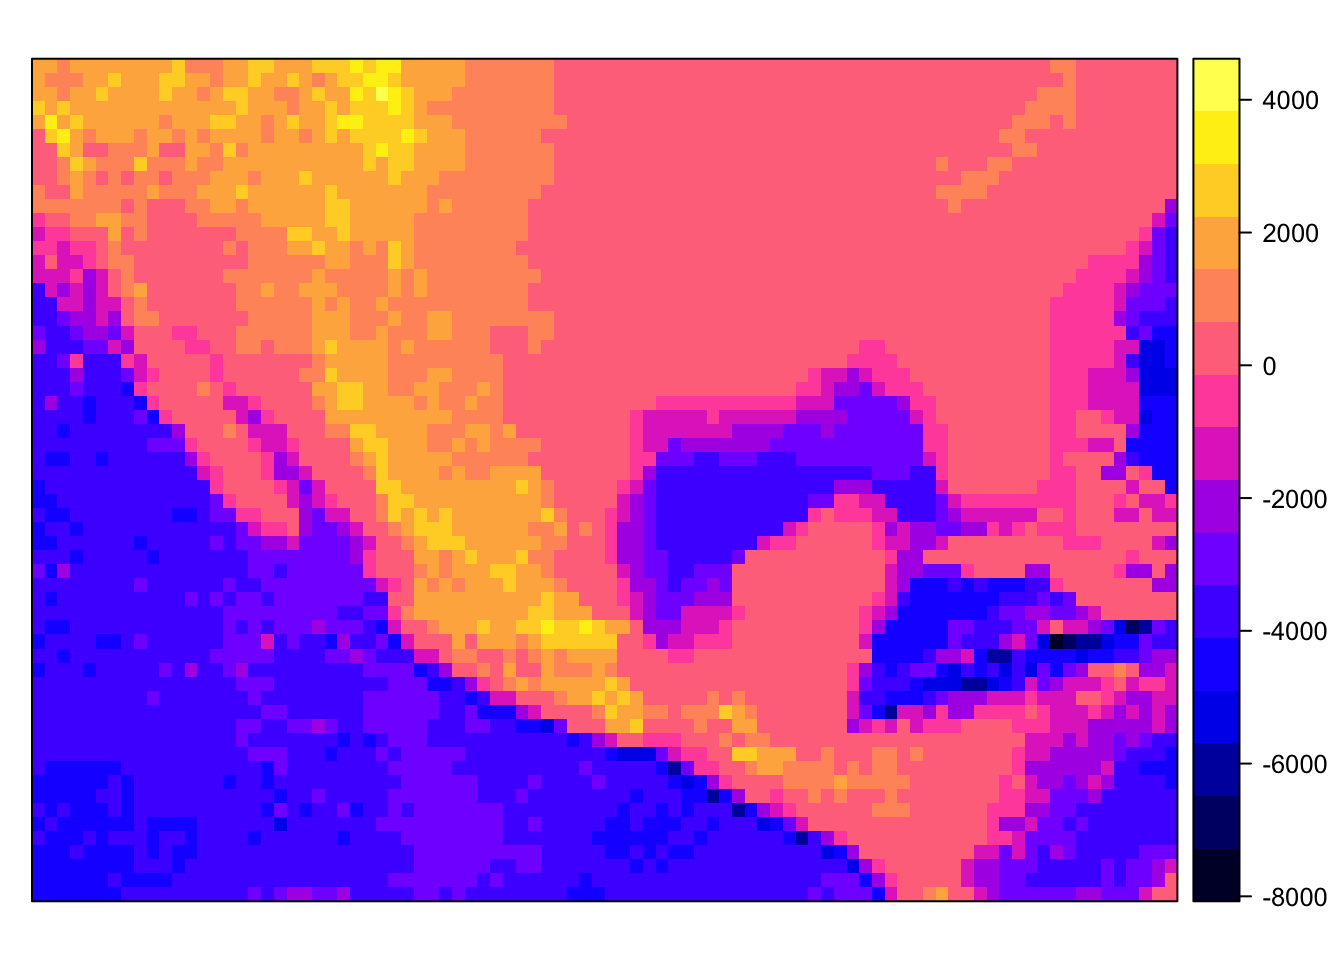
\includegraphics{04-TablesDataReading_files/figure-latex/unnamed-chunk-2-1.pdf}

Существуют более специальные функции для чтения таблиц \textbf{CSV}:
\texttt{read.csv()} и \texttt{read.csv2()}. По сути они являются
``обертками'' (\emph{wrappers}) функции \texttt{read.table()} и
выполняют ее вызов с автоматической подстановкой параметров
\texttt{sep}, \texttt{dec} и \texttt{header}. Обе функции по умолчанию
предполагают, что в файле имеется заголовок. \texttt{read.csv()} удобна
для чтения таблиц с десятичной точкой и запятой-разделителем, а
\texttt{read.csv2()} --- для таблиц с десятичной запятой и
точкой-с-запятой в качестве разделителя.

Используем для чтения \texttt{read.csv2()}:

\begin{Shaded}
\begin{Highlighting}[]
\NormalTok{tab2<-}\KeywordTok{read.csv2}\NormalTok{(}\StringTok{"oxr_vod.csv"}\NormalTok{, }\DataTypeTok{encoding =} \StringTok{'UTF-8'}\NormalTok{)}
\end{Highlighting}
\end{Shaded}

\begin{Shaded}
\begin{Highlighting}[]
\KeywordTok{View}\NormalTok{(tab2)}
\end{Highlighting}
\end{Shaded}

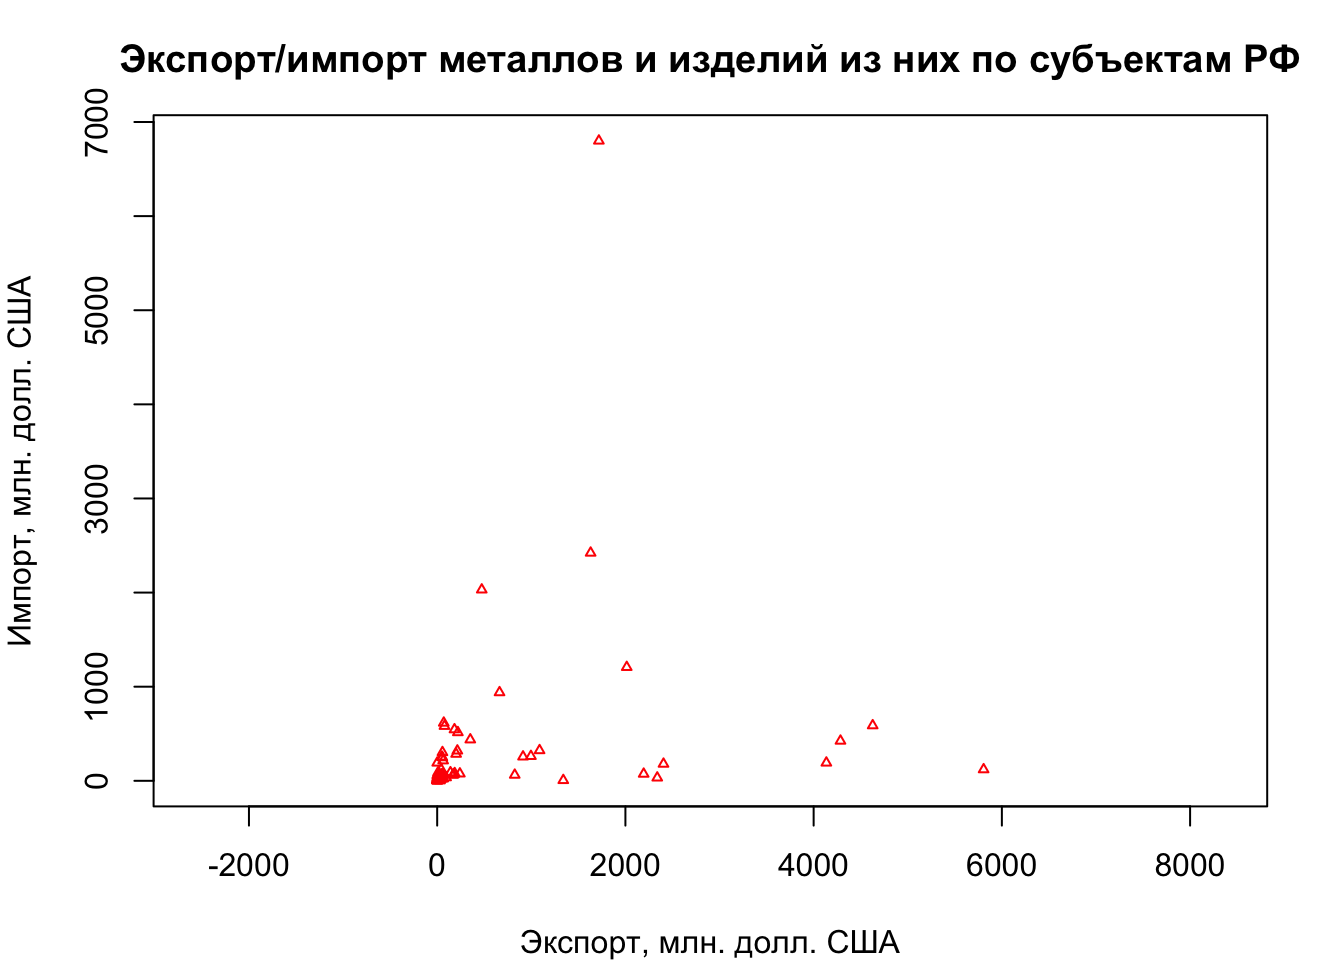
\includegraphics{04-TablesDataReading_files/figure-latex/unnamed-chunk-5-1.pdf}
Как видно, данная таблица не отличается от предыдущей, но ее чтение
более компактно.

\section{Фильтрация, сортировка, работа с элементами
таблицы}\label{filtering_sorting}

Распространенные операции с таблицами --- это упорядочение по
определенному столбцу и фильтрация по значениям. Мы уже знаем что из
вектора, матрицы или таблицы можно извлекать элементы:
\texttt{tab{[}V,\ {]}}, где \texttt{tab} --- имя таблицы, \texttt{V} ---
это вектор из номеров элементов. Например, извлечь 5, 2 и 4 строку
таблицы можно так:

\begin{Shaded}
\begin{Highlighting}[]
\NormalTok{tab[}\KeywordTok{c}\NormalTok{(}\DecValTok{5}\NormalTok{,}\DecValTok{2}\NormalTok{,}\DecValTok{4}\NormalTok{), ]}
\NormalTok{##    Год Всего Балтийское Черное Азовское Каспийское Карское Белое Прочие}
\NormalTok{## 5 1997  23.0        2.2    0.3      3.8        9.8     4.4   0.8    1.7}
\NormalTok{## 2 1994  24.6        2.3    0.4      3.2       11.0     5.0   0.9    1.8}
\NormalTok{## 4 1996  22.4        2.2    0.3      3.1        9.8     4.7   0.8    1.5}
\end{Highlighting}
\end{Shaded}

Логично предположить, что таким же образом можно извлечь элементы
таблицы в порядке, обеспечивающем возрастание или убывание значений в
каком-то столбце. Для этого нужно правильным образом расставить индексы
в векторе \texttt{c(...)}. Существует специальная функция
\texttt{order()}, которая позволяет это сделать. Например, отсортируем
таблицу по возрастанию сбросов в Каспийское море:

\begin{Shaded}
\begin{Highlighting}[]
\NormalTok{indexes<-}\KeywordTok{order}\NormalTok{(tab}\OperatorTok{$}\NormalTok{Каспийское)}
\KeywordTok{head}\NormalTok{(tab[indexes, ])}
\NormalTok{##     Год Всего Балтийское Черное Азовское Каспийское Карское Белое Прочие}
\NormalTok{## 22 2014  14.8        1.7    0.2      1.5        6.4     3.2   0.6    1.2}
\NormalTok{## 17 2009  15.9        1.8    0.2      1.5        6.8     3.5   0.7    1.4}
\NormalTok{## 21 2013  15.2        1.8    0.2      1.6        6.9     3.0   0.6    1.1}
\NormalTok{## 20 2012  15.7        1.8    0.2      1.6        7.0     3.0   0.7    1.4}
\NormalTok{## 19 2011  16.0        1.9    0.2      1.6        7.1     3.2   0.7    1.3}
\NormalTok{## 18 2010  16.5        2.0    0.2      1.6        7.3     3.3   0.7    1.4}
\end{Highlighting}
\end{Shaded}

\begin{quote}
Используйте функцию \texttt{head()}, чтобы отобразить первые несколько
строк таблицы. Эта возможность особенно полезна при работе с большими
таблицами
\end{quote}

Если упорядочение несложное, программист его скорее всего вставит
непосредственно в инструкцию обращения к таблице:

\begin{Shaded}
\begin{Highlighting}[]
\KeywordTok{head}\NormalTok{(tab[}\KeywordTok{order}\NormalTok{(tab}\OperatorTok{$}\NormalTok{Каспийское), ])}
\NormalTok{##     Год Всего Балтийское Черное Азовское Каспийское Карское Белое Прочие}
\NormalTok{## 22 2014  14.8        1.7    0.2      1.5        6.4     3.2   0.6    1.2}
\NormalTok{## 17 2009  15.9        1.8    0.2      1.5        6.8     3.5   0.7    1.4}
\NormalTok{## 21 2013  15.2        1.8    0.2      1.6        6.9     3.0   0.6    1.1}
\NormalTok{## 20 2012  15.7        1.8    0.2      1.6        7.0     3.0   0.7    1.4}
\NormalTok{## 19 2011  16.0        1.9    0.2      1.6        7.1     3.2   0.7    1.3}
\NormalTok{## 18 2010  16.5        2.0    0.2      1.6        7.3     3.3   0.7    1.4}
\end{Highlighting}
\end{Shaded}

Схожим образом реализована \emph{фильтрация данных} по значению.
Например, вы хотите извлечь из таблицы только те года, в которых объем
сбросов в Каспийское море составил более 10 млн м\(^3\). Здесь
используется еще одна возможность извлечения элементов таблицы --- с
помощью вектора логических значений \texttt{TRUE/FALSE}. Число элементов
в этом векторе должно быть равно числу элементов в индексируемом
векторе, а значение указывает на то, нужно ли извлекать (\texttt{TRUE})
или нет (\texttt{FALSE}) элемент с текущим индексом. Вектор логических
значений получается естественным путем с помощью операции сравнения:

\begin{Shaded}
\begin{Highlighting}[]
\NormalTok{condition <-}\StringTok{ }\NormalTok{tab}\OperatorTok{$}\NormalTok{Каспийское }\OperatorTok{>}\StringTok{ }\DecValTok{10}
\NormalTok{condition  }\CommentTok{# посмотрим что получилось}
\NormalTok{##  [1]  TRUE  TRUE  TRUE FALSE FALSE FALSE FALSE FALSE FALSE FALSE FALSE}
\NormalTok{## [12] FALSE FALSE FALSE FALSE FALSE FALSE FALSE FALSE FALSE FALSE FALSE}
\NormalTok{tab[condition, ] }\CommentTok{# используем его для фильтрации строк таблицы:}
\NormalTok{##    Год Всего Балтийское Черное Азовское Каспийское Карское Белое Прочие}
\NormalTok{## 1 1993  27.2        2.5    0.4      4.3       12.1     5.3   1.0    1.6}
\NormalTok{## 2 1994  24.6        2.3    0.4      3.2       11.0     5.0   0.9    1.8}
\NormalTok{## 3 1995  24.5        2.3    0.4      3.5       10.4     5.2   0.9    1.8}
\end{Highlighting}
\end{Shaded}

Опять же, весьма часто используется запись одним выражением:

\begin{Shaded}
\begin{Highlighting}[]
\NormalTok{tab[tab}\OperatorTok{$}\NormalTok{Каспийское }\OperatorTok{>}\StringTok{ }\DecValTok{10}\NormalTok{, ]}
\NormalTok{##    Год Всего Балтийское Черное Азовское Каспийское Карское Белое Прочие}
\NormalTok{## 1 1993  27.2        2.5    0.4      4.3       12.1     5.3   1.0    1.6}
\NormalTok{## 2 1994  24.6        2.3    0.4      3.2       11.0     5.0   0.9    1.8}
\NormalTok{## 3 1995  24.5        2.3    0.4      3.5       10.4     5.2   0.9    1.8}
\end{Highlighting}
\end{Shaded}

Можно создать новую таблицу, выбрав необходимые столбцы:

\begin{Shaded}
\begin{Highlighting}[]
\NormalTok{caspian <-}\StringTok{ }\KeywordTok{data.frame}\NormalTok{(tab}\OperatorTok{$}\NormalTok{Год, tab}\OperatorTok{$}\NormalTok{Всего, tab}\OperatorTok{$}\NormalTok{Каспийское)}
\end{Highlighting}
\end{Shaded}

Следует заметить, что не рекомендуется использовать кириллические
названия столбцов (см. \protect\hyperlink{table_rules}{Правила
подготовки таблиц для чтения в R} в конце данного модуля), поэтому
переименуем их:

\begin{Shaded}
\begin{Highlighting}[]
\KeywordTok{colnames}\NormalTok{(caspian)<-}\KeywordTok{c}\NormalTok{(}\StringTok{"Year"}\NormalTok{, }\StringTok{"Total"}\NormalTok{, }\StringTok{"Caspian"}\NormalTok{)}
\end{Highlighting}
\end{Shaded}

Предположим, что теперь нам необходимо вычислить долю сбросов в
Каспийское море в общем объеме и записать ее в новый столбец с точностью
до 3 знаков после запятой. Для этого сначала произведем вычисления:

\begin{Shaded}
\begin{Highlighting}[]
\NormalTok{ratio <-}\StringTok{ }\NormalTok{caspian}\OperatorTok{$}\NormalTok{Caspian }\OperatorTok{/}\StringTok{ }\NormalTok{caspian}\OperatorTok{$}\NormalTok{Total}
\NormalTok{ratio}
\NormalTok{##  [1] 0.4448529 0.4471545 0.4244898 0.4375000 0.4260870 0.4318182 0.4396135}
\NormalTok{##  [8] 0.4532020 0.4494949 0.4646465 0.4421053 0.4486486 0.4519774 0.4457143}
\NormalTok{## [15] 0.4302326 0.4385965 0.4276730 0.4424242 0.4437500 0.4458599 0.4539474}
\NormalTok{## [22] 0.4324324}
\end{Highlighting}
\end{Shaded}

Далее округлим результат с помощью функции \texttt{round()} с параметром
\texttt{digits}, указывающим число значащих цифр в ответе:

\begin{Shaded}
\begin{Highlighting}[]
\NormalTok{ratio <-}\StringTok{ }\KeywordTok{round}\NormalTok{(ratio, }\DataTypeTok{digits =} \DecValTok{3}\NormalTok{)}
\NormalTok{ratio}
\NormalTok{##  [1] 0.445 0.447 0.424 0.438 0.426 0.432 0.440 0.453 0.449 0.465 0.442}
\NormalTok{## [12] 0.449 0.452 0.446 0.430 0.439 0.428 0.442 0.444 0.446 0.454 0.432}
\end{Highlighting}
\end{Shaded}

Существует простой и элегантный способ создать новый столбец в таблице
--- достаточно указать его название после значка \texttt{\$}. Если среда
R не обнаруживает столбец с таким названием, она его создаст:

\begin{Shaded}
\begin{Highlighting}[]
\NormalTok{caspian}\OperatorTok{$}\NormalTok{CaspianRatio <-}\StringTok{ }\NormalTok{ratio}
\end{Highlighting}
\end{Shaded}

\begin{Shaded}
\begin{Highlighting}[]
\KeywordTok{View}\NormalTok{(caspian)}
\end{Highlighting}
\end{Shaded}

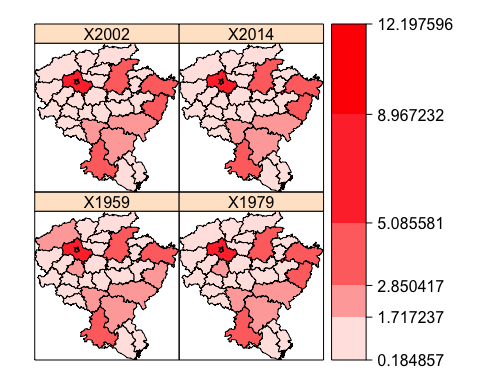
\includegraphics{04-TablesDataReading_files/figure-latex/unnamed-chunk-17-1.pdf}
К столбцу таблицы можно обращаться по номеру, а не названию. Если вы
указываете в квадратных скобках номер без запятой, он трактуется как
номер столбца. При этом возвращаемый столбец имеет тип
\texttt{data.frame}:

\begin{Shaded}
\begin{Highlighting}[]
\KeywordTok{head}\NormalTok{(caspian[}\DecValTok{2}\NormalTok{])  }\CommentTok{# второй столбец (фактически — таблица из одного столбца)}
\NormalTok{##   Total}
\NormalTok{## 1  27.2}
\NormalTok{## 2  24.6}
\NormalTok{## 3  24.5}
\NormalTok{## 4  22.4}
\NormalTok{## 5  23.0}
\NormalTok{## 6  22.0}
\KeywordTok{head}\NormalTok{(caspian[}\KeywordTok{c}\NormalTok{(}\DecValTok{1}\NormalTok{,}\DecValTok{4}\NormalTok{)])  }\CommentTok{# первый и четвертый столбец}
\NormalTok{##   Year CaspianRatio}
\NormalTok{## 1 1993        0.445}
\NormalTok{## 2 1994        0.447}
\NormalTok{## 3 1995        0.424}
\NormalTok{## 4 1996        0.438}
\NormalTok{## 5 1997        0.426}
\NormalTok{## 6 1998        0.432}
\end{Highlighting}
\end{Shaded}

В противоположность этому, более привычная форма обращения к двумерным
данным через запятую приведет к тому, что столбец будет возвращен как
вектор:

\begin{Shaded}
\begin{Highlighting}[]
\NormalTok{caspian[,}\DecValTok{2}\NormalTok{]}
\NormalTok{##  [1] 27.2 24.6 24.5 22.4 23.0 22.0 20.7 20.3 19.8 19.8 19.0 18.5 17.7 17.5}
\NormalTok{## [15] 17.2 17.1 15.9 16.5 16.0 15.7 15.2 14.8}
\end{Highlighting}
\end{Shaded}

Использование той или иной формы зависит от контекста.

\section{Чтение таблиц Microsoft Excel}\label{excel_reading}

Чтение таблиц \textbf{Microsoft Excel} производится с помощью функции
\texttt{read.xlsx()} из пакета \texttt{openxlsx}. В качестве
обязательных параметров они принимают следующие аргументы:

\begin{itemize}
\tightlist
\item
  \texttt{xlsxFile} --- название файла
\item
  \texttt{sheet} --- номер листа
\end{itemize}

Убедитесь, что у вас установлена и подключена библиотека
\texttt{openxlsx}.

Откроем таблицу с данными Росстата по сбросу загрязненных сточных вод в
поверхностные водные объекты (млн м\(^3\)).

\begin{Shaded}
\begin{Highlighting}[]
\KeywordTok{library}\NormalTok{(openxlsx)}
\NormalTok{sewage<-}\KeywordTok{read.xlsx}\NormalTok{(}\StringTok{"sewage.xlsx"}\NormalTok{,}\DecValTok{1}\NormalTok{) }\CommentTok{# Читаем таблицу из первого листа}
\NormalTok{## Warning in read.xlsx.default("sewage.xlsx", 1): '.Random.seed' не является}
\NormalTok{## целочисленным вектором, он типа 'NULL', и поэтому пропущен}
\end{Highlighting}
\end{Shaded}

\begin{Shaded}
\begin{Highlighting}[]
\KeywordTok{View}\NormalTok{(sewage)}
\end{Highlighting}
\end{Shaded}

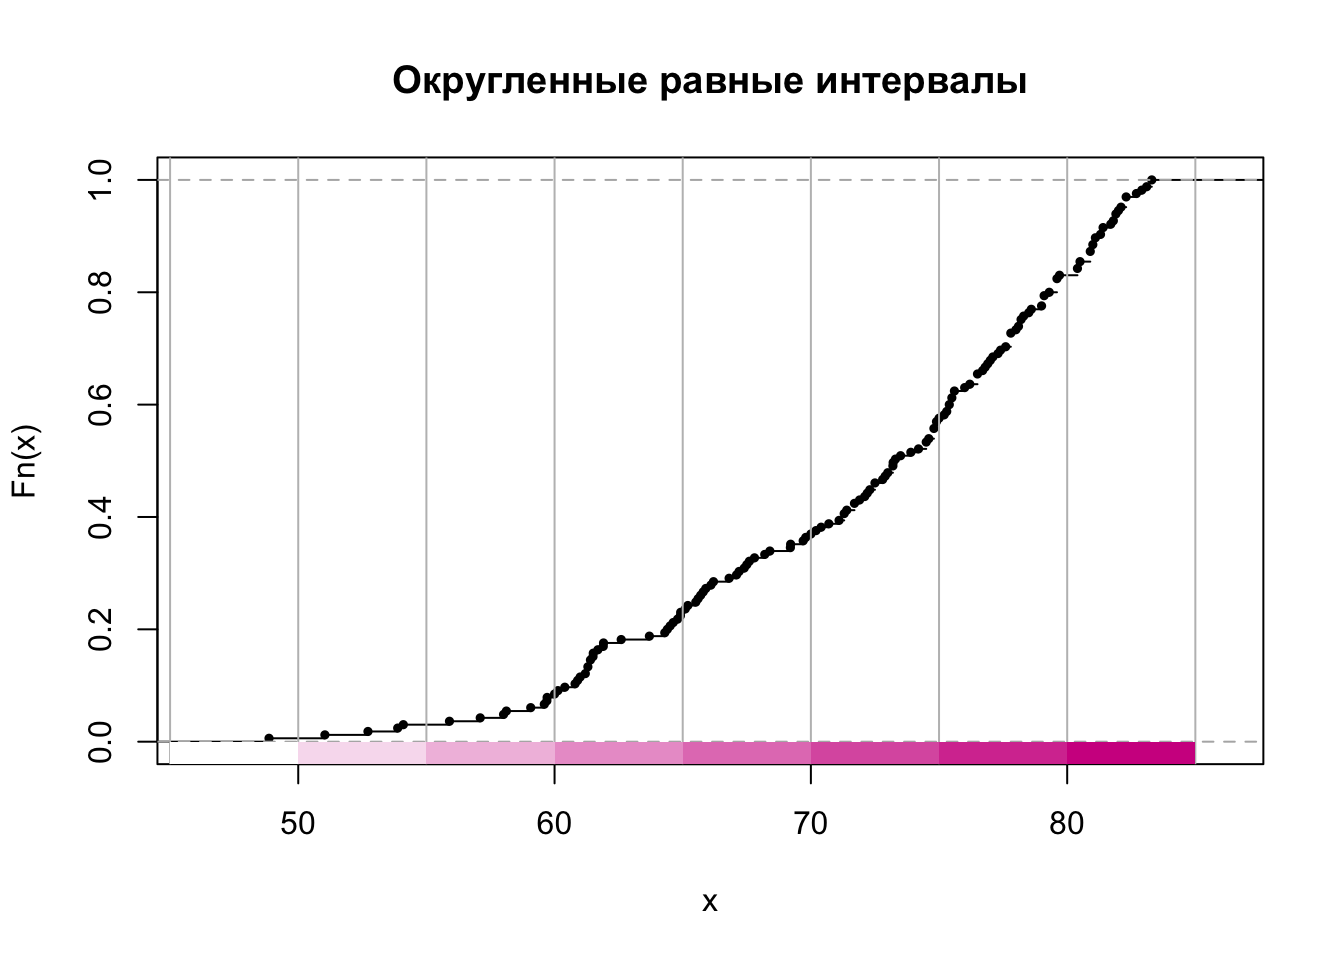
\includegraphics{04-TablesDataReading_files/figure-latex/unnamed-chunk-22-1.pdf}
Следует дать адекватные названия столбцам таблицы:

\begin{Shaded}
\begin{Highlighting}[]
\KeywordTok{colnames}\NormalTok{(sewage) <-}\StringTok{ }\KeywordTok{c}\NormalTok{(}\StringTok{"Region"}\NormalTok{, }\StringTok{"Year05"}\NormalTok{, }\StringTok{"Year10"}\NormalTok{, }\StringTok{"Year11"}\NormalTok{, }\StringTok{"Year12"}\NormalTok{, }\StringTok{"Year13"}\NormalTok{)}
\end{Highlighting}
\end{Shaded}

\begin{Shaded}
\begin{Highlighting}[]
\KeywordTok{View}\NormalTok{(sewage)}
\end{Highlighting}
\end{Shaded}

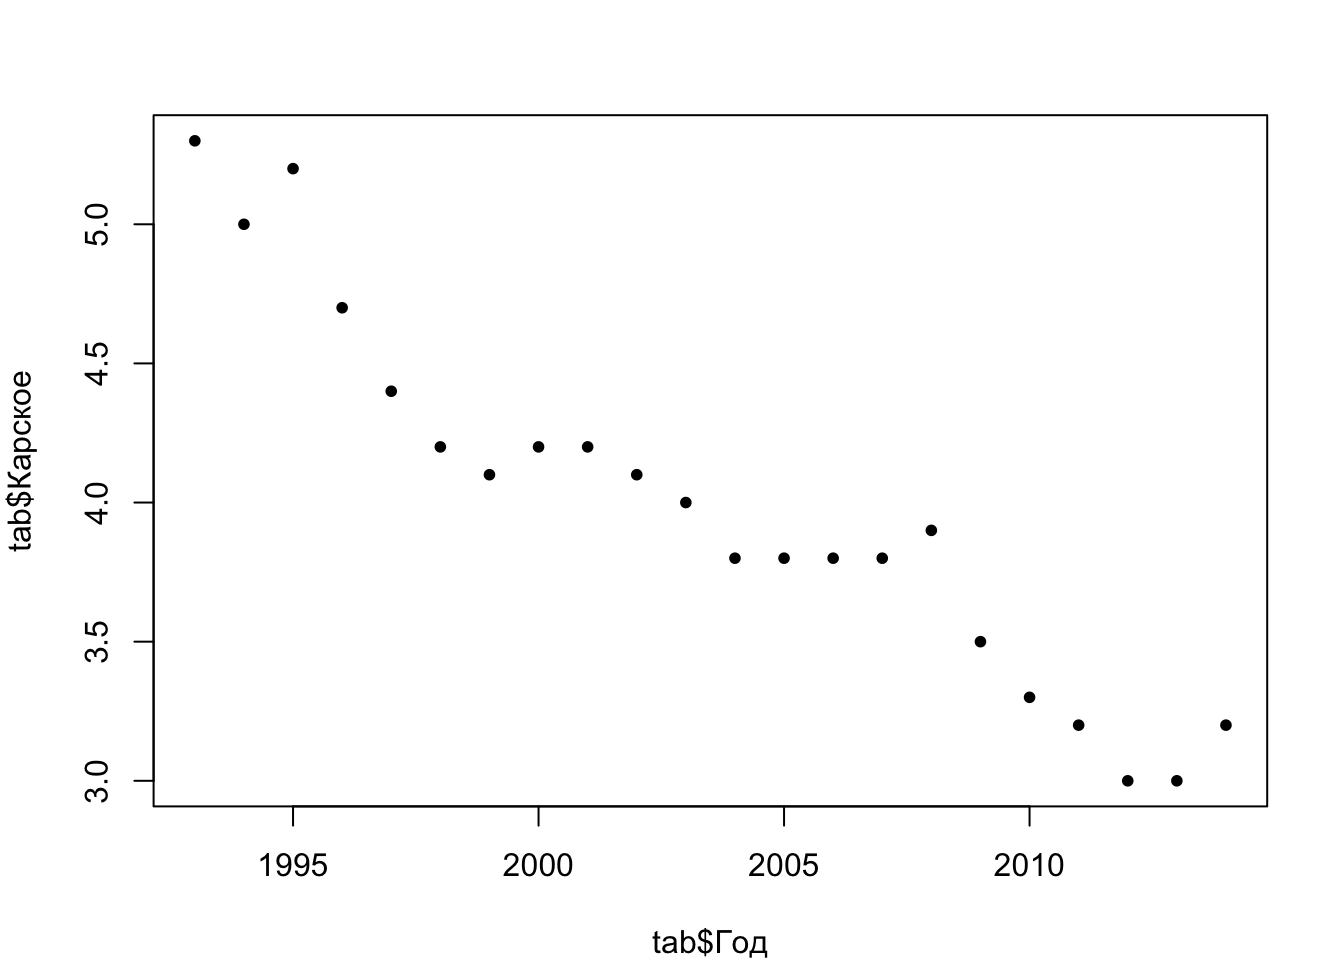
\includegraphics{04-TablesDataReading_files/figure-latex/unnamed-chunk-25-1.pdf}

\section{Пропущенные значения}\label{missed_values}

Можно ли осуществлять обработку таблицы \texttt{sewage}? Попробуем в
качестве примера найти минимум сбросов за 2012 год:

\begin{Shaded}
\begin{Highlighting}[]
\KeywordTok{max}\NormalTok{(sewage}\OperatorTok{$}\NormalTok{Year12)}
\NormalTok{## [1] NA}
\end{Highlighting}
\end{Shaded}

Результат имеет тип \texttt{NA}, потому что в данном столбце имеются
пропуски. В некоторых статистических задачах это недопустимо. Если вы
хотите проигнорировать значения пропусков, следует в вызываемой
статистической функции указать дополнительный параметр
\texttt{na.rm\ =\ TRUE}:

\begin{Shaded}
\begin{Highlighting}[]
\KeywordTok{max}\NormalTok{(sewage}\OperatorTok{$}\NormalTok{Year13, }\DataTypeTok{na.rm =} \OtherTok{TRUE}\NormalTok{)}
\NormalTok{## [1] 15189}
\end{Highlighting}
\end{Shaded}

Еще один вариант --- исключить из таблицы те строки, в которых имеются
пропущенные значения (хотя бы одно!). Для этого существует функция
\texttt{complete.cases()}, возвращающая вектор логических значений:

\begin{Shaded}
\begin{Highlighting}[]
\NormalTok{filter<-}\KeywordTok{complete.cases}\NormalTok{(sewage)}
\NormalTok{filter  }\CommentTok{# посмотрим что получилось. Там где видим FALSE - есть пропуски в строках}
\NormalTok{##  [1]  TRUE  TRUE  TRUE  TRUE  TRUE  TRUE  TRUE  TRUE  TRUE  TRUE  TRUE}
\NormalTok{## [12]  TRUE  TRUE  TRUE  TRUE  TRUE  TRUE  TRUE  TRUE  TRUE  TRUE  TRUE}
\NormalTok{## [23]  TRUE  TRUE FALSE  TRUE  TRUE  TRUE  TRUE  TRUE  TRUE  TRUE  TRUE}
\NormalTok{## [34]  TRUE  TRUE  TRUE  TRUE  TRUE  TRUE  TRUE  TRUE  TRUE  TRUE  TRUE}
\NormalTok{## [45]  TRUE  TRUE  TRUE  TRUE  TRUE  TRUE  TRUE  TRUE  TRUE  TRUE  TRUE}
\NormalTok{## [56]  TRUE  TRUE  TRUE  TRUE  TRUE  TRUE  TRUE  TRUE  TRUE  TRUE  TRUE}
\NormalTok{## [67]  TRUE FALSE  TRUE  TRUE  TRUE  TRUE  TRUE  TRUE  TRUE  TRUE  TRUE}
\NormalTok{## [78]  TRUE  TRUE  TRUE  TRUE  TRUE  TRUE  TRUE  TRUE  TRUE  TRUE  TRUE}
\NormalTok{## [89]  TRUE  TRUE  TRUE  TRUE  TRUE  TRUE  TRUE FALSE FALSE}

\NormalTok{sewage.complete <-}\StringTok{ }\NormalTok{sewage[filter, ] }\CommentTok{# отфильтруем полные строки}
\end{Highlighting}
\end{Shaded}

\begin{Shaded}
\begin{Highlighting}[]
\KeywordTok{View}\NormalTok{(sewage.complete)}
\end{Highlighting}
\end{Shaded}

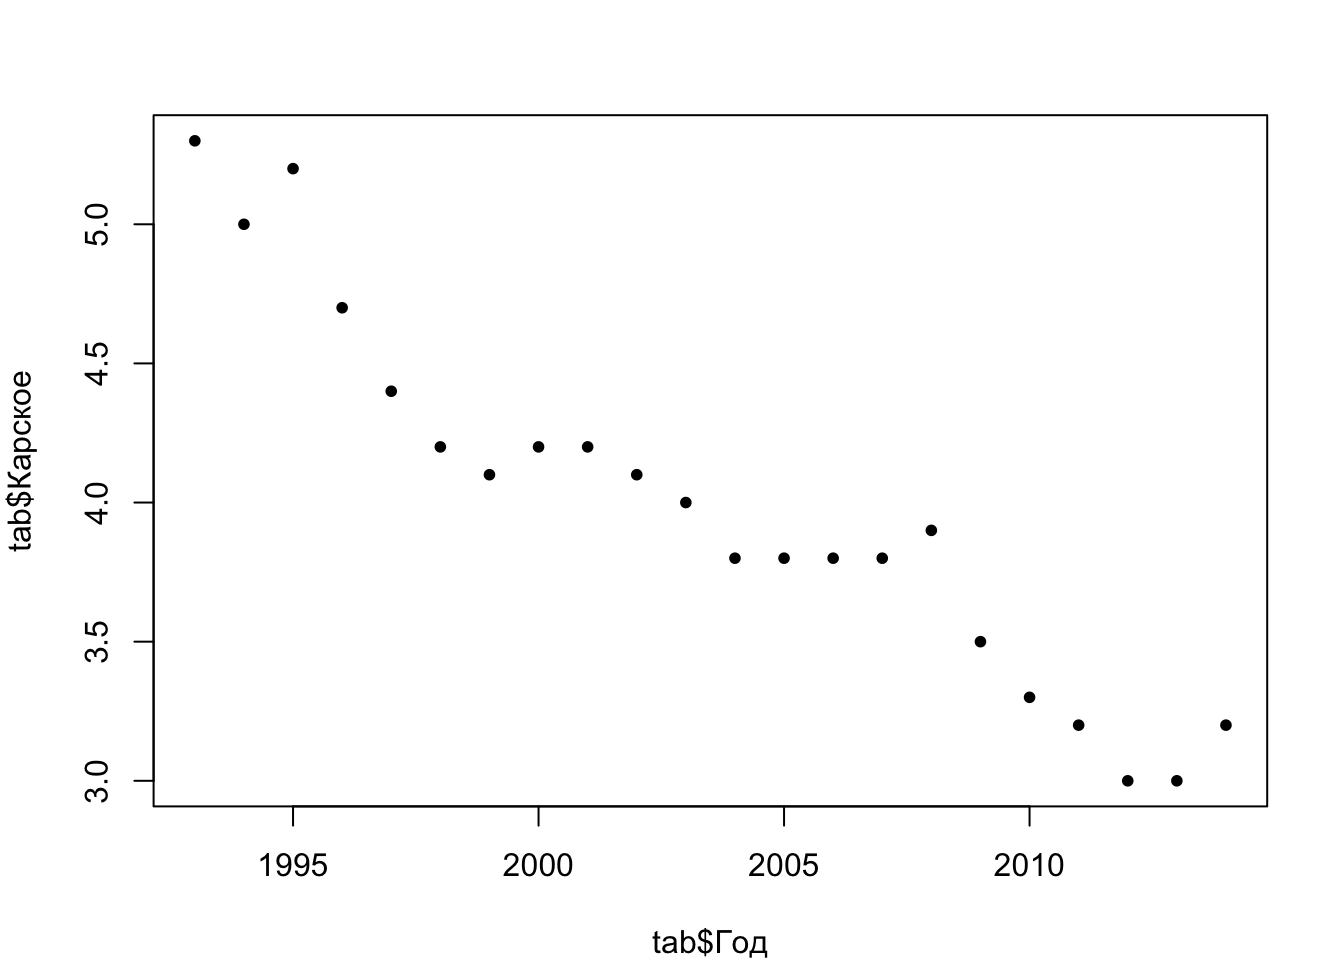
\includegraphics{04-TablesDataReading_files/figure-latex/unnamed-chunk-30-1.pdf}

\section{Фильтрация по текстовым полям}\label{filtering_text}

Часто бывает необходимо отобрать данные из таблицы, содержащей
разнородные данные. В частности, в нашей таблице смешаны данные по
субъектам и федеральным округам. Предположим, необходимо выгрузить в
отдельную таблицу данные по федеральным округам. Для этого нужно найти
строки, в которых столбец \texttt{Region} содержит фразу
\texttt{"федеральный\ округ"}. Для поиска по текстовым эталонам
импользуется функция \texttt{grep()}, выдающая номера элементов, или ее
разновидность \texttt{grepl()}, выдающая список логических констант

\begin{Shaded}
\begin{Highlighting}[]
\CommentTok{# Первый параметр - искомое выражение, второй параметр - где искть}
\NormalTok{rows <-}\StringTok{ }\KeywordTok{grep}\NormalTok{(}\StringTok{"федеральный округ"}\NormalTok{,sewage}\OperatorTok{$}\NormalTok{Region)}
\NormalTok{rows  }\CommentTok{# посмотрим, какие элементы столбца Region ему соответствуют}
\NormalTok{## [1]  2 21 35 42 49 64 73 86}
\NormalTok{okruga <-}\StringTok{ }\NormalTok{sewage[rows,] }\CommentTok{# отфильтруем найденные строки}
\end{Highlighting}
\end{Shaded}

\begin{Shaded}
\begin{Highlighting}[]
\KeywordTok{View}\NormalTok{(okruga)}
\end{Highlighting}
\end{Shaded}

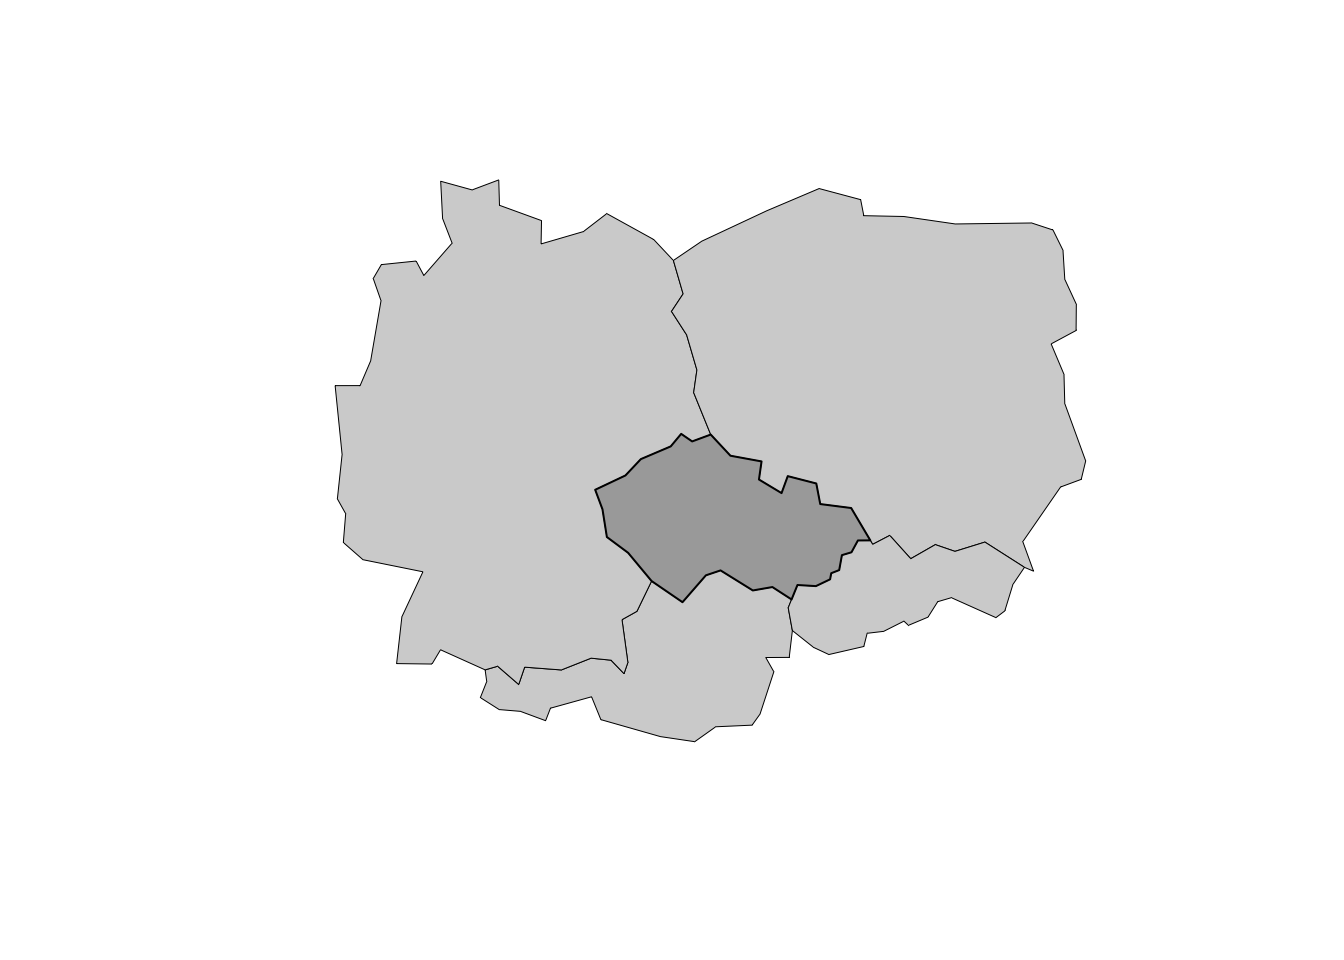
\includegraphics{04-TablesDataReading_files/figure-latex/unnamed-chunk-33-1.pdf}
Наоборот --- для \textbf{исключения} найденных объектов удобнее
воспользоваться разновидностью \texttt{grepl()}, которая возвращает
вектор из логических значений:

\begin{Shaded}
\begin{Highlighting}[]
\NormalTok{rows2 <-}\StringTok{ }\KeywordTok{grepl}\NormalTok{(}\StringTok{"федеральный округ"}\NormalTok{,sewage}\OperatorTok{$}\NormalTok{Region)}
\NormalTok{rows2 }\CommentTok{# вот так выглядит результат grepl}
\NormalTok{##  [1] FALSE  TRUE FALSE FALSE FALSE FALSE FALSE FALSE FALSE FALSE FALSE}
\NormalTok{## [12] FALSE FALSE FALSE FALSE FALSE FALSE FALSE FALSE FALSE  TRUE FALSE}
\NormalTok{## [23] FALSE FALSE FALSE FALSE FALSE FALSE FALSE FALSE FALSE FALSE FALSE}
\NormalTok{## [34] FALSE  TRUE FALSE FALSE FALSE FALSE FALSE FALSE  TRUE FALSE FALSE}
\NormalTok{## [45] FALSE FALSE FALSE FALSE  TRUE FALSE FALSE FALSE FALSE FALSE FALSE}
\NormalTok{## [56] FALSE FALSE FALSE FALSE FALSE FALSE FALSE FALSE  TRUE FALSE FALSE}
\NormalTok{## [67] FALSE FALSE FALSE FALSE FALSE FALSE  TRUE FALSE FALSE FALSE FALSE}
\NormalTok{## [78] FALSE FALSE FALSE FALSE FALSE FALSE FALSE FALSE  TRUE FALSE FALSE}
\NormalTok{## [89] FALSE FALSE FALSE FALSE FALSE FALSE FALSE FALSE FALSE}

\NormalTok{neokruga <-}\StringTok{ }\NormalTok{sewage[}\OperatorTok{!}\NormalTok{rows2,]}
\end{Highlighting}
\end{Shaded}

\begin{Shaded}
\begin{Highlighting}[]
\KeywordTok{View}\NormalTok{(neokruga)}
\end{Highlighting}
\end{Shaded}

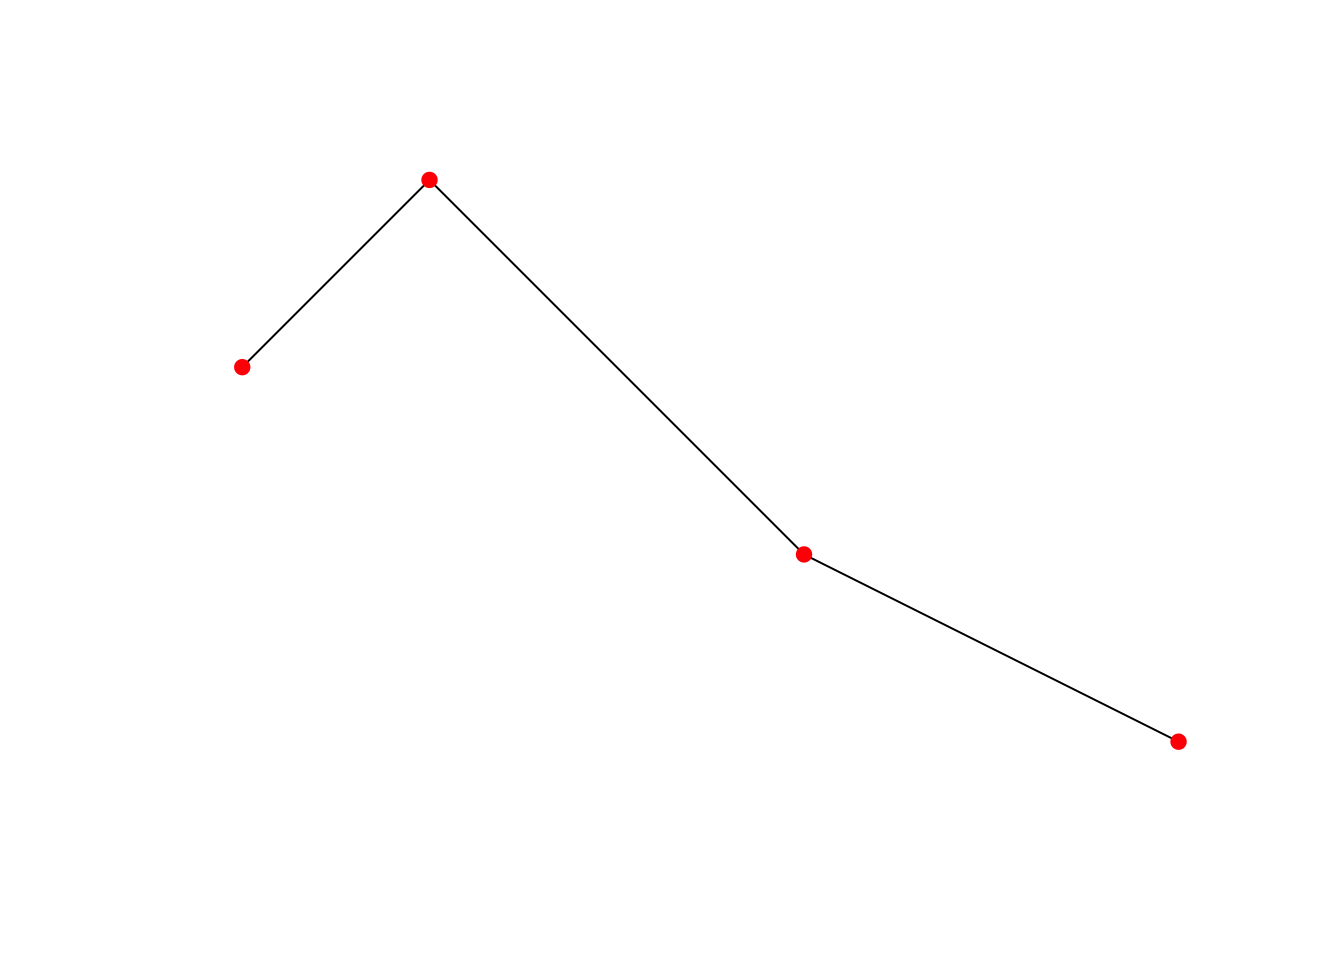
\includegraphics{04-TablesDataReading_files/figure-latex/unnamed-chunk-36-1.pdf}
Обратите внимание на восклицательный знак перед \texttt{rows2}. Он
меняет все значения \texttt{TRUE} на \texttt{FALSE} и наоборот, что
позволяет исключить найденные объекты

В полученной таблице все еще содержится текстовая шелуха типа
\texttt{"в\ том\ числе"}, \texttt{"Данные\ за..."}, а также строка
\texttt{"Российская\ Федерация"}. К счастью, функция \texttt{grep()}
достаточо умна и возволяет искать сразу по нескольким образцам строк.
Для этого их нужно разделить вертикальной чертой --- \emph{пайпом}
(\texttt{\textbar{}}):

\begin{Shaded}
\begin{Highlighting}[]
\NormalTok{rows2 <-}\StringTok{ }\KeywordTok{grepl}\NormalTok{(}\StringTok{"федеральный|числе|Российская|за|ѕ"}\NormalTok{,sewage}\OperatorTok{$}\NormalTok{Region)}
\NormalTok{rows2}
\NormalTok{##  [1]  TRUE  TRUE FALSE FALSE FALSE FALSE FALSE FALSE FALSE FALSE FALSE}
\NormalTok{## [12] FALSE FALSE  TRUE FALSE FALSE FALSE FALSE FALSE FALSE  TRUE FALSE}
\NormalTok{## [23] FALSE FALSE  TRUE FALSE FALSE FALSE FALSE FALSE FALSE FALSE FALSE}
\NormalTok{## [34] FALSE  TRUE FALSE FALSE FALSE FALSE FALSE FALSE  TRUE FALSE FALSE}
\NormalTok{## [45] FALSE FALSE FALSE FALSE  TRUE FALSE FALSE FALSE FALSE FALSE FALSE}
\NormalTok{## [56] FALSE FALSE FALSE FALSE FALSE FALSE FALSE FALSE  TRUE FALSE FALSE}
\NormalTok{## [67] FALSE  TRUE FALSE FALSE FALSE FALSE  TRUE FALSE FALSE FALSE FALSE}
\NormalTok{## [78] FALSE FALSE FALSE FALSE FALSE FALSE FALSE FALSE  TRUE FALSE FALSE}
\NormalTok{## [89] FALSE FALSE FALSE FALSE FALSE FALSE FALSE  TRUE  TRUE}
\NormalTok{neokruga <-}\StringTok{ }\NormalTok{sewage[}\OperatorTok{!}\NormalTok{rows2,] }\CommentTok{# обратите внимание на восклицательный знак перед rows2}
\end{Highlighting}
\end{Shaded}

\begin{Shaded}
\begin{Highlighting}[]
\KeywordTok{View}\NormalTok{(neokruga)}
\end{Highlighting}
\end{Shaded}

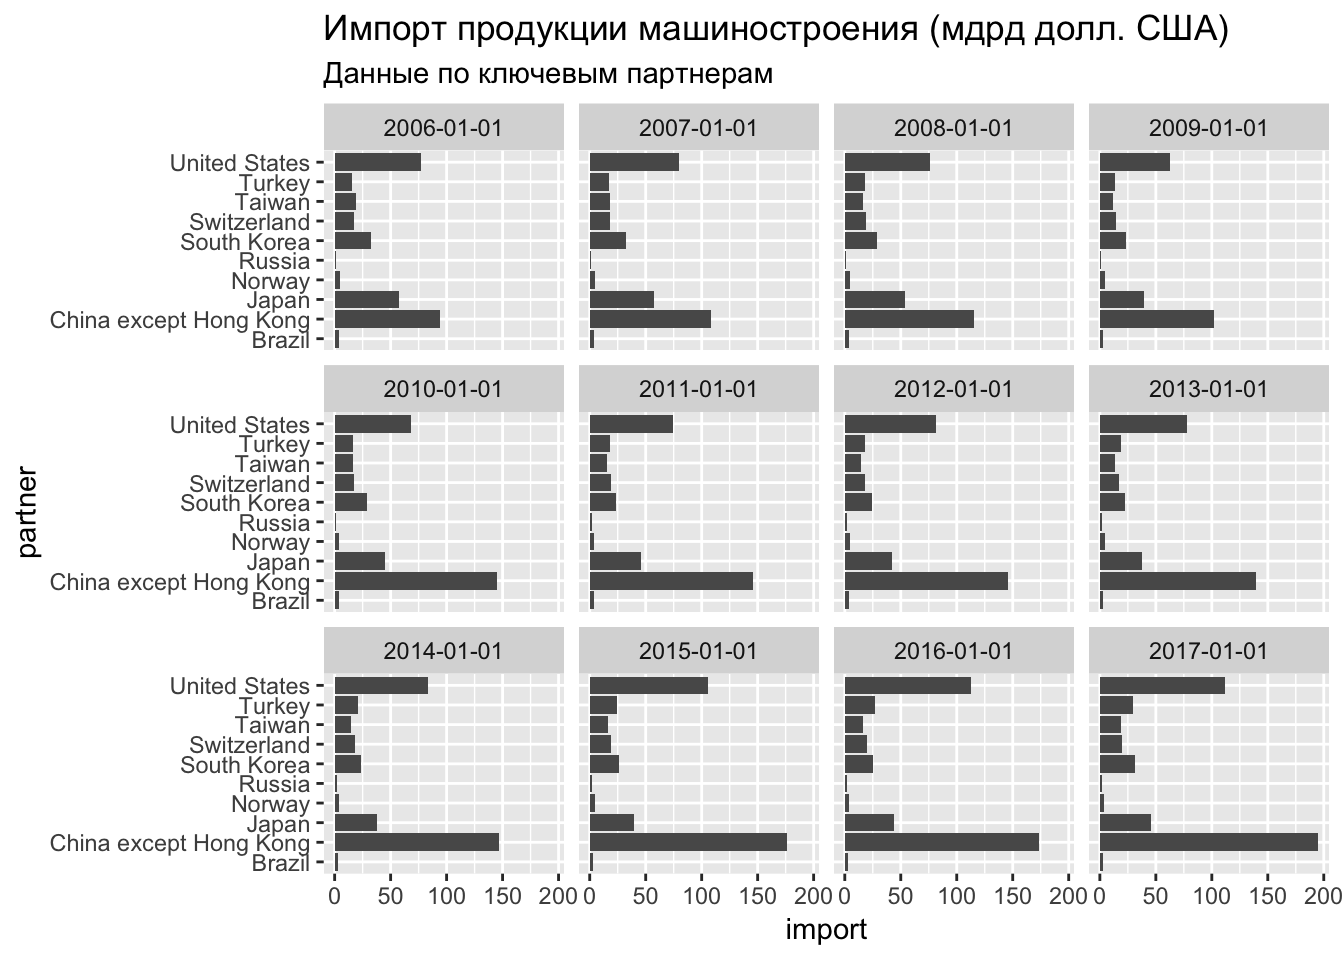
\includegraphics{04-TablesDataReading_files/figure-latex/unnamed-chunk-39-1.pdf}

\section{Преобразование типов данных и исправление
ошибок}\label{data_conversion}

Достаточно часто при работе с реальными данными возникает необходимость
преобразования их типов. Например, вам необходимо перевести строки в
даты, чтобы оперировать ими соответствующим образом. Или принудительным
образом указать, что столбец со строками не хранит номинальную
переменную (фактор), а его нужно интерпретировать именно как строковый
столбец (обычно это полезно, когда столбец содержит какую-то текстовую
информацию в виде комментариев по каждому измерению). Наконец, в данных
могут быть ошибки, опечатки и так далее, которые могут препятствовать
правильному их чтению.

В этом разделе мы рассмотрим, как можно:

\begin{enumerate}
\def\labelenumi{\arabic{enumi}.}
\tightlist
\item
  Найти и исправить множественные варианты одного названия с опечатками
\item
  Исправить ошибки в числовых данных
\item
  Преобразовать факторы в строки и наоборот
\item
  Преобразовать строки в числа и наоборот
\end{enumerate}

Рассмотрим возможные манипуляции с данными на примере таблицы о
землепользовании на территории Сатинского учебного полигоны
Географического факультета МГУ:

\begin{Shaded}
\begin{Highlighting}[]
\NormalTok{tab <-}\StringTok{ }\KeywordTok{read.csv2}\NormalTok{(}\StringTok{"SatinoLanduse.csv"}\NormalTok{, }\DataTypeTok{encoding =} \StringTok{'UTF-8'}\NormalTok{)}
\KeywordTok{str}\NormalTok{(tab) }\CommentTok{# посмотрим, какова структура данных}
\NormalTok{## 'data.frame':    160 obs. of  6 variables:}
\NormalTok{##  $ ID            : int  1 2 3 4 5 6 7 8 9 10 ...}
\NormalTok{##  $ Type          : Factor w/ 12 levels "Выгоны","Вырубки",..: 11 1 1 9 5 1 5 12 9 10 ...}
\NormalTok{##  $ Administration: Factor w/ 7 levels "","РФ","Совьяковская администрация",..: 5 5 5 1 1 5 1 5 5 6 ...}
\NormalTok{##  $ Comment       : Factor w/ 35 levels "","АО \textbackslash{}"Родина\textbackslash{}"",..: 30 1 1 1 1 1 1 3 2 1 ...}
\NormalTok{##  $ Perimeter     : Factor w/ 160 levels "1014.155593894044800",..: 67 155 51 104 78 153 17 19 108 57 ...}
\NormalTok{##  $ Area          : Factor w/ 160 levels "0.238070145845919",..: 73 49 121 100 63 72 88 128 99 24 ...}
\end{Highlighting}
\end{Shaded}

\begin{Shaded}
\begin{Highlighting}[]
\KeywordTok{View}\NormalTok{(tab)}
\end{Highlighting}
\end{Shaded}

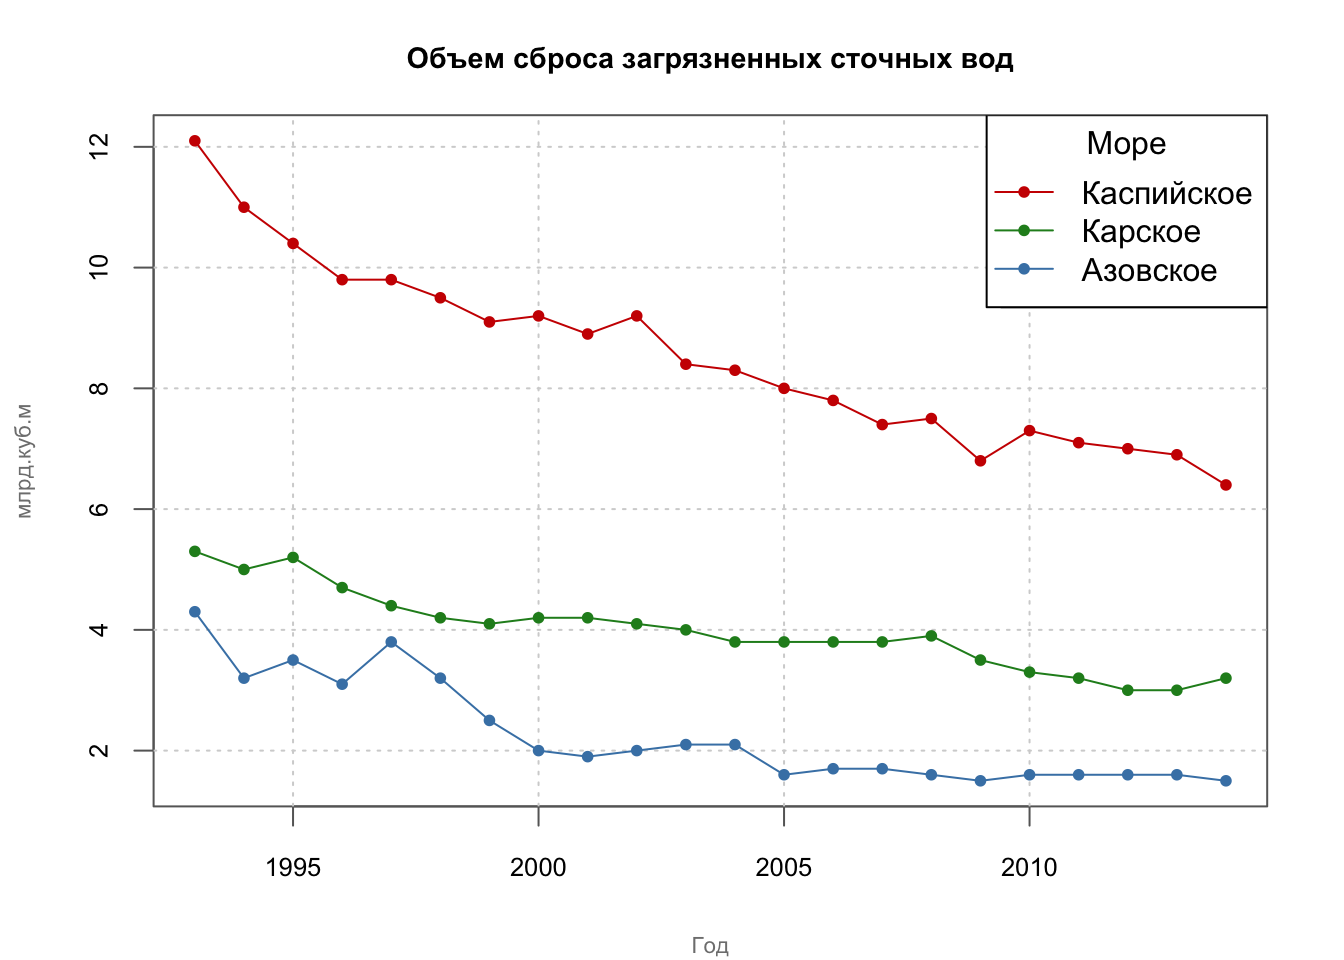
\includegraphics{04-TablesDataReading_files/figure-latex/unnamed-chunk-42-1.pdf}
Видно, что все столбцы, кроме двух, хранящих идентификаторы, были
прочитаны как строки и преобразованы в факторы (номинальные переменные).
Это означает, что мы не сможем работать привычным образом со столбцами
периметра и площади, а столбец комментариев теперь также является
номинальной переменной, что противоречит здравому смыслу (он вообще
переменной не является).

Когда вы отображаете таблицу в консоли или графическом интерфейсе,
факторы выглядят и ведут себя как обычные строки. Подвох заключается в
том, что хранятся они в виде пар ``ключ --- значение'' (об этом мы
говорили выше) и все операции преобразования осуществляются \textbf{над
ключами}, а не значениями. Рассмотрим, как следует правильно
преобразовывать номинальные переменные в \textbf{R}.

Чтобы привести столбцы к нужному типу, необходимо использовать
преобразования типов. Для этого в \textbf{R} существует множество
функций семейства \texttt{as(object,class)}, где в качестве первого
параметра \texttt{object} вы указываете преобразуемый объект, а в
качестве второго параметра \texttt{class} --- тип, к которому вы хотите
его привести. Например:

\begin{Shaded}
\begin{Highlighting}[]
\NormalTok{s <-}\StringTok{ "5456.788"}
\NormalTok{s }\OperatorTok{+}\StringTok{ }\DecValTok{1}
\NormalTok{## Error in s + 1: нечисловой аргумент для бинарного оператора}
\NormalTok{n <-}\StringTok{ }\KeywordTok{as}\NormalTok{(s, }\StringTok{"numeric"}\NormalTok{)}
\NormalTok{## Error in as(s, "numeric"): не могу найти функцию "as"}
\NormalTok{n }\OperatorTok{+}\StringTok{ }\DecValTok{1}
\NormalTok{## Error in eval(expr, envir, enclos): объект 'n' не найден}
\NormalTok{s <-}\StringTok{ }\KeywordTok{as}\NormalTok{(n, }\StringTok{"character"}\NormalTok{)}
\NormalTok{## Error in as(n, "character"): не могу найти функцию "as"}
\NormalTok{s}
\NormalTok{## [1] "5456.788"}
\KeywordTok{nchar}\NormalTok{(s)}
\NormalTok{## [1] 8}
\end{Highlighting}
\end{Shaded}

На практике обычно пользуются не функцией \texttt{as()}, а ее обертками
(\emph{wrappers}), которые имеют вид \texttt{as.numeric()},
\texttt{as.character()}, \texttt{as.Date()} и так далее:

\begin{Shaded}
\begin{Highlighting}[]
\KeywordTok{as.numeric}\NormalTok{(s) }\CommentTok{# то же самое, что и as(s, "numeric")}
\NormalTok{## [1] 5456.788}
\end{Highlighting}
\end{Shaded}

Для начала преобразуем столбец \texttt{Comment} к обычному символьному
представлению:

\begin{Shaded}
\begin{Highlighting}[]
\NormalTok{tab}\OperatorTok{$}\NormalTok{Comment <-}\StringTok{ }\KeywordTok{as.character}\NormalTok{(tab}\OperatorTok{$}\NormalTok{Comment)}
\KeywordTok{str}\NormalTok{(tab)}
\NormalTok{## 'data.frame':    160 obs. of  6 variables:}
\NormalTok{##  $ ID            : int  1 2 3 4 5 6 7 8 9 10 ...}
\NormalTok{##  $ Type          : Factor w/ 12 levels "Выгоны","Вырубки",..: 11 1 1 9 5 1 5 12 9 10 ...}
\NormalTok{##  $ Administration: Factor w/ 7 levels "","РФ","Совьяковская администрация",..: 5 5 5 1 1 5 1 5 5 6 ...}
\NormalTok{##  $ Comment       : chr  "Село Беницы" "" "" "" ...}
\NormalTok{##  $ Perimeter     : Factor w/ 160 levels "1014.155593894044800",..: 67 155 51 104 78 153 17 19 108 57 ...}
\NormalTok{##  $ Area          : Factor w/ 160 levels "0.238070145845919",..: 73 49 121 100 63 72 88 128 99 24 ...}
\end{Highlighting}
\end{Shaded}

Посмотрим теперь, что произойдет, если мы попытаемся преобразовать
столбец \texttt{Perimeter} к числовому виду:

\begin{Shaded}
\begin{Highlighting}[]
\KeywordTok{as.numeric}\NormalTok{(tab}\OperatorTok{$}\NormalTok{Perimeter)}
\NormalTok{##   [1]  67 155  51 104  78 153  17  19 108  57   7   3 158 159 156  50  91}
\NormalTok{##  [18] 143   6  58   4   5 131 148 113 128 147 114   9  18 118 132  84 134}
\NormalTok{##  [35]  81  40 130  98  83 157  42  95  71 141   8 100  34   1  87  77 160}
\NormalTok{##  [52]  93 119  90  74  35 125 150 101 136  31 109 110 103  75  14  32  63}
\NormalTok{##  [69] 145  56 102  25  65  88  72  53  92  30 117  73  43  54 121  44  52}
\NormalTok{##  [86]  27 115 149 120  45  26  41   2  60  36 123  29 151 144 106 127  12}
\NormalTok{## [103] 116  94  82 146 142  69  21  48 139 105 154 124  47  61  33  80  97}
\NormalTok{## [120]  64  10  76 111  11 112  89  28 129  68  39  49  86  96  59  24 137}
\NormalTok{## [137]  46 152  55  15  99  85  22 126  16 122  79  66 133  23 107  38 138}
\NormalTok{## [154]  13 135  37 140  70  20  62}
\end{Highlighting}
\end{Shaded}

Вместо значений перметра мы получили загадочные числа, которых в таблице
нет. Это и есть ключи факторов. Чтобы получить их значения, необходимо
использовать функцию \texttt{levels()} (для краткости выведем первые 10
значений):

\begin{Shaded}
\begin{Highlighting}[]
\KeywordTok{levels}\NormalTok{(tab}\OperatorTok{$}\NormalTok{Perimeter)[}\DecValTok{1}\OperatorTok{:}\DecValTok{10}\NormalTok{]}
\NormalTok{##  [1] "1014.155593894044800" "1019.457949256323400" "1020.278536197552200"}
\NormalTok{##  [4] "1021.109926202218700" "1041.122684298658400" "1060.678503301135200"}
\NormalTok{##  [7] "1081.964408568060900" "1094.945610298295600" "114.701418496307100" }
\NormalTok{## [10] "1155.916232728818800"}
\end{Highlighting}
\end{Shaded}

Обратите внимание на то, что значения фактора отсортированы в алфавитном
порядке, без учете порядка их встречаемости в исходной таблице. Для
корректного преобразования факторов в числа необходимо сначала привести
их к обычному строковому виду:

\begin{Shaded}
\begin{Highlighting}[]
\NormalTok{tab}\OperatorTok{$}\NormalTok{Perimeter <-}\StringTok{ }\KeywordTok{as.numeric}\NormalTok{(}\KeywordTok{as.character}\NormalTok{(tab}\OperatorTok{$}\NormalTok{Perimeter))}
\KeywordTok{str}\NormalTok{(tab)}
\NormalTok{## 'data.frame':    160 obs. of  6 variables:}
\NormalTok{##  $ ID            : int  1 2 3 4 5 6 7 8 9 10 ...}
\NormalTok{##  $ Type          : Factor w/ 12 levels "Выгоны","Вырубки",..: 11 1 1 9 5 1 5 12 9 10 ...}
\NormalTok{##  $ Administration: Factor w/ 7 levels "","РФ","Совьяковская администрация",..: 5 5 5 1 1 5 1 5 5 6 ...}
\NormalTok{##  $ Comment       : chr  "Село Беницы" "" "" "" ...}
\NormalTok{##  $ Perimeter     : num  2396 922 2181 3948 279 ...}
\NormalTok{##  $ Area          : Factor w/ 160 levels "0.238070145845919",..: 73 49 121 100 63 72 88 128 99 24 ...}

\CommentTok{# Теперь попробуем преобразовать столбец Area}
\NormalTok{temp <-}\StringTok{ }\KeywordTok{as.numeric}\NormalTok{(}\KeywordTok{as.character}\NormalTok{(tab}\OperatorTok{$}\NormalTok{Area))}
\NormalTok{## Warning: в результате преобразования созданы NA}
\NormalTok{temp[}\DecValTok{1}\OperatorTok{:}\DecValTok{10}\NormalTok{]}
\NormalTok{##  [1]  286159.159   21651.964   56826.463  450293.759    2612.615}
\NormalTok{##  [6]   28608.401 3469445.793   62299.631  450291.261  147943.134}
\end{Highlighting}
\end{Shaded}

Все прошло вроде бы успешно, но с предупреждением, что некоторые
значения были преобразованы в \texttt{NA} (\emph{Not Available}) ---
отсутствующие значения. По всей видимости, данные в соответствущих
ячейках не соответствуют представлениям \textbf{R} о том, как должно
выглядеть число: ячейка или пустая, или число набрано с
ошибкой/опечаткой.

Чтобы найти и исправить все неверно заданные данные, необходимо
выполнить следующие действия:

\begin{enumerate}
\def\labelenumi{\arabic{enumi}.}
\tightlist
\item
  Получить индексы всех элементов, имеющих значение \texttt{NA}.
\item
  Просмотреть, какие значения были в исходных данных под этими индексами
\item
  Исправить ошибки в этих значениях, если это поддается автоматизации
\item
  Повторить конвертацию в числовой тип данных
\end{enumerate}

Проверку на отсутствующие данные осуществляют с помощью функции
\texttt{is.na()}. Передав ей в качестве аргумента вектор значений, вы
получите вектор булевых значений, в котором \texttt{TRUE} будет стоять
для пустых элементов. Проверим с помощью него, какие элементы столюца
\texttt{Area} привели к ошибкам конвертации данных:

\begin{Shaded}
\begin{Highlighting}[]
\NormalTok{tab[}\KeywordTok{is.na}\NormalTok{(temp), }\StringTok{"Area"}\NormalTok{]}
\NormalTok{## [1] 89499,573298880117000 11922,638460079328000 5153,570673500797100 }
\NormalTok{## 160 Levels: 0.238070145845919 ... 9865.323033935605100}
\end{Highlighting}
\end{Shaded}

Видно, что \textbf{R} не справился с преобразованием типов там, где
содержится опечатка в десятичном разделителе --- вместо точки указана
запятая.

Для исправления этой ошибки мы можем воспользоваться стандартной
функцией замены символа \texttt{gsub(pattern,\ replacement,\ x)}. Ее
стандартные параметры означают соответственно: что искать, на что
заменять, где искать:

\begin{Shaded}
\begin{Highlighting}[]
\NormalTok{tab}\OperatorTok{$}\NormalTok{Area <-}\StringTok{ }\KeywordTok{gsub}\NormalTok{(}\StringTok{','}\NormalTok{, }\StringTok{'.'}\NormalTok{, tab}\OperatorTok{$}\NormalTok{Area) }\CommentTok{# заменим запятые на точки}
\NormalTok{tab}\OperatorTok{$}\NormalTok{Area <-}\StringTok{ }\KeywordTok{as.numeric}\NormalTok{(}\KeywordTok{as.character}\NormalTok{(tab}\OperatorTok{$}\NormalTok{Area)) }\CommentTok{# Теперь можно преобразовать в числа}
\KeywordTok{str}\NormalTok{(tab)}
\NormalTok{## 'data.frame':    160 obs. of  6 variables:}
\NormalTok{##  $ ID            : int  1 2 3 4 5 6 7 8 9 10 ...}
\NormalTok{##  $ Type          : Factor w/ 12 levels "Выгоны","Вырубки",..: 11 1 1 9 5 1 5 12 9 10 ...}
\NormalTok{##  $ Administration: Factor w/ 7 levels "","РФ","Совьяковская администрация",..: 5 5 5 1 1 5 1 5 5 6 ...}
\NormalTok{##  $ Comment       : chr  "Село Беницы" "" "" "" ...}
\NormalTok{##  $ Perimeter     : num  2396 922 2181 3948 279 ...}
\NormalTok{##  $ Area          : num  286159 21652 56826 450294 2613 ...}
\end{Highlighting}
\end{Shaded}

Теперь необходимо навести порядок в значениях факторов, убедившись, что
и там нет опечаток. Выведем все уникальные значения с помощью функции
\texttt{levels()}:

\begin{Shaded}
\begin{Highlighting}[]
\KeywordTok{levels}\NormalTok{(tab}\OperatorTok{$}\NormalTok{Type)}
\NormalTok{##  [1] "Выгоны"                        "Вырубки"                      }
\NormalTok{##  [3] "Гидрологические объекты"       "Заболоченные земли"           }
\NormalTok{##  [5] "Леса"                          "Лесные поляны"                }
\NormalTok{##  [7] "Луга"                          "Нет данных"                   }
\NormalTok{##  [9] "Пашни"                         "Сады"                         }
\NormalTok{## [11] "Территории населенных пунктов" "Фермерские хозяйства"}
\KeywordTok{levels}\NormalTok{(tab}\OperatorTok{$}\NormalTok{Administration)}
\NormalTok{## [1] ""                                    }
\NormalTok{## [2] "РФ"                                  }
\NormalTok{## [3] "Совьяковская администрация"          }
\NormalTok{## [4] "Совьяковская сельскаая администрация"}
\NormalTok{## [5] "Совьяковская сельская администрация" }
\NormalTok{## [6] "Совьяковская сельская Администрация" }
\NormalTok{## [7] "Совьяковская сельская админитрация"}
\end{Highlighting}
\end{Shaded}

Видно, что если с типами все в порядке, то в данных об административном
подчинении содержится 5 вариантов названия одной и той же Совьяковской
сельской администрации. Помимо этого, пустые ячейки хорошо бы заменить
на значение \texttt{"Прочее"}.

Чтобы найти все строчки, относящиеся к одному и тому же объекту, можно
воспользоваться уже знакомой нам функцией \texttt{grep()}, передав ей
подстроку, которая является для них общей. Например,
\texttt{"Совьяковская"} (хотя в данном случае было бы вообще достаточно
одной буквы \texttt{"с"}).

\begin{Shaded}
\begin{Highlighting}[]
\NormalTok{filter <-}\StringTok{ }\KeywordTok{grep}\NormalTok{(}\StringTok{"Совьяковская"}\NormalTok{, tab}\OperatorTok{$}\NormalTok{Administration) }\CommentTok{# Найдем все записи}
\NormalTok{tab[filter, }\StringTok{"Administration"}\NormalTok{] <-}\StringTok{ "Совьяковская сельская администрация"} \CommentTok{# Заменим их одним значением}
\NormalTok{tab}\OperatorTok{$}\NormalTok{Administration <-}\StringTok{ }\KeywordTok{droplevels}\NormalTok{(tab}\OperatorTok{$}\NormalTok{Administration) }\CommentTok{# Удаляем неиспользуемые уровни}
\KeywordTok{levels}\NormalTok{(tab}\OperatorTok{$}\NormalTok{Administration)}
\NormalTok{## [1] ""                                   }
\NormalTok{## [2] "РФ"                                 }
\NormalTok{## [3] "Совьяковская сельская администрация"}
\end{Highlighting}
\end{Shaded}

Пустые строки можно также найти c помощью \texttt{grep()}, но мы этого
делать не будем, так как это требует дополнительных знаний о регулярных
выражениях. Вместо этого воспользуемся тем, что пустые строки имеют
длину 0. Обратите внимание ниже, что преобразование в вектор столбца
\texttt{Administration} необходимо, т.к. \texttt{nchar()} не понимает
объекты типа \texttt{data.frame}, которыми являются не только таблицы,
но и их столбцы:

\begin{Shaded}
\begin{Highlighting}[]
\NormalTok{filter <-}\StringTok{ }\KeywordTok{nchar}\NormalTok{(}\KeywordTok{as.vector}\NormalTok{(tab}\OperatorTok{$}\NormalTok{Administration)) }\OperatorTok{==}\StringTok{ }\DecValTok{0} \CommentTok{# TRUE если длина равна 0}
\CommentTok{# Пробуем заменить:}
\NormalTok{tab[filter, }\StringTok{"Administration"}\NormalTok{] <-}\StringTok{ "Прочее"}
\NormalTok{## Warning in `[<-.factor`(`*tmp*`, iseq, value = c("Прочее", "Прочее", :}
\NormalTok{## неправильный уровень фактора, получились NA}
\end{Highlighting}
\end{Shaded}

Ошибка выше связана с тем, что \textbf{R} строго следит за неизменностью
набора значений фактора для того чтобы избежать всевозможных ошибок при
работе с данными (опечаток и т.д.). Предыдущий раз мы заменили все
значаниея одним из существующих. В данном случае необходимо ввести новое
значение фактора. Чтобы это сделать, придется преобразовать данные в
символьные, произвести замену срок и после этого снова конвертировать
столбец в фактор:

\begin{Shaded}
\begin{Highlighting}[]
\NormalTok{tab}\OperatorTok{$}\NormalTok{Administration <-}\StringTok{ }\KeywordTok{as.character}\NormalTok{(tab}\OperatorTok{$}\NormalTok{Administration)}
\NormalTok{tab[filter, }\StringTok{"Administration"}\NormalTok{] <-}\StringTok{ "Прочее"}
\NormalTok{tab}\OperatorTok{$}\NormalTok{Administration <-}\StringTok{ }\KeywordTok{as.factor}\NormalTok{(tab}\OperatorTok{$}\NormalTok{Administration)}
\KeywordTok{levels}\NormalTok{(tab}\OperatorTok{$}\NormalTok{Administration)}
\NormalTok{## [1] "Прочее"                             }
\NormalTok{## [2] "РФ"                                 }
\NormalTok{## [3] "Совьяковская сельская администрация"}
\end{Highlighting}
\end{Shaded}

Теперь таблица готова к работе. Можно, например, подсчитать по ней
сводную статистику:

\begin{Shaded}
\begin{Highlighting}[]
\KeywordTok{summary}\NormalTok{(tab)}
\NormalTok{##        ID                                    Type   }
\NormalTok{##  Min.   :  1.00   Леса                         :52  }
\NormalTok{##  1st Qu.: 40.75   Выгоны                       :27  }
\NormalTok{##  Median : 80.50   Фермерские хозяйства         :22  }
\NormalTok{##  Mean   : 80.50   Пашни                        :15  }
\NormalTok{##  3rd Qu.:120.25   Луга                         :11  }
\NormalTok{##  Max.   :160.00   Территории населенных пунктов: 8  }
\NormalTok{##                   (Other)                      :25  }
\NormalTok{##                              Administration   Comment         }
\NormalTok{##  Прочее                             :76     Length:160        }
\NormalTok{##  РФ                                 : 3     Class :character  }
\NormalTok{##  Совьяковская сельская администрация:81     Mode  :character  }
\NormalTok{##                                                               }
\NormalTok{##                                                               }
\NormalTok{##                                                               }
\NormalTok{##                                                               }
\NormalTok{##    Perimeter              Area        }
\NormalTok{##  Min.   :    3.087   Min.   :      0  }
\NormalTok{##  1st Qu.:  421.431   1st Qu.:   5087  }
\NormalTok{##  Median :  939.369   Median :  21260  }
\NormalTok{##  Mean   : 1761.654   Mean   : 125002  }
\NormalTok{##  3rd Qu.: 2135.987   3rd Qu.:  83019  }
\NormalTok{##  Max.   :23920.945   Max.   :3469446  }
\NormalTok{## }
\end{Highlighting}
\end{Shaded}

Обратите внимание, что строки, интервальные и номинальные (факторы)
переменные обрабатываются функцией \texttt{summary()} по-разному.

\section{Сохранение таблиц CSV и Microsoft Excel}\label{table_writing}

Одной из завершающих стадий анализа данных, помимо графиков и отчетов,
часто являются новые табличные представления, которые было бы неплохо
сохранить в виде файлов. К счастью, сохранение таблиц в \textbf{R} столь
же просто, как и чтение. Для текстовых файлов в формате \textbf{CSV}
можно использовать функции \texttt{write.table()}, \texttt{write.csv()}
и \texttt{write.csv2()}. Для файлов \textbf{Microsoft Excel} используйте
функцию \texttt{write.xlsx()} из пакета \texttt{openxlsx}
соответственно.

\begin{quote}
По умолчанию функции \texttt{write.table()}, \texttt{write.csv()} и
\texttt{write.csv2()} записывают в таблицы в качестве первого столбца
названия (номера) строк таблиц. Если вы не хотите, чтобы это
происходило, укажите дополнительный параметр \texttt{row.names=FALSE}.
\end{quote}

Сохраним таблицы \texttt{okruga} и \texttt{neokruga}, раздельно хранящие
статистику по объему сброса сточных в поверхностные водные объекты по
федеральным округам и субъектам соответственно:

\begin{Shaded}
\begin{Highlighting}[]
\KeywordTok{write.csv2}\NormalTok{(okruga, }\StringTok{"okruga.csv"}\NormalTok{, }\DataTypeTok{fileEncoding =} \StringTok{'UTF-8'}\NormalTok{) }\CommentTok{# Сохраним первую таблицу в CSV в кодировке Unicode}
\KeywordTok{write.xlsx}\NormalTok{(neokruga, }\StringTok{"neokruga.xlsx"}\NormalTok{) }\CommentTok{# Сохраним вторую таблицу в XLSX без названий строк}

\CommentTok{# Проверим, все ли в порядке с сохраненными таблицами:}

\NormalTok{okruga.saved <-}\StringTok{ }\KeywordTok{read.csv2}\NormalTok{(}\StringTok{"okruga.csv"}\NormalTok{, }\DataTypeTok{encoding =} \StringTok{'UTF-8'}\NormalTok{)}
\KeywordTok{head}\NormalTok{(okruga.saved)}
\NormalTok{##    X                               Region Year05 Year10 Year11 Year12}
\NormalTok{## 1  2       Центральный федеральный округ    4341   3761   3613   3651}
\NormalTok{## 2 21   Северо-Западный федеральный округ    3192   3088   2866   2877}
\NormalTok{## 3 35             Южный федеральный округ    1409   1446   1436   1394}
\NormalTok{## 4 42 Северо-Кавказский федеральный округ     496    390    397    395}
\NormalTok{## 5 49       Приволжский федеральный округ    3162   2883   2857   2854}
\NormalTok{## 6 64         Уральский федеральный округ    1681   1860   1834   1665}
\NormalTok{##   Year13}
\NormalTok{## 1   3570}
\NormalTok{## 2   2796}
\NormalTok{## 3   1321}
\NormalTok{## 4    374}
\NormalTok{## 5   2849}
\NormalTok{## 6   1624}

\NormalTok{neokruga.saved <-}\StringTok{ }\KeywordTok{read.xlsx}\NormalTok{(}\StringTok{"neokruga.xlsx"}\NormalTok{,}\DecValTok{1}\NormalTok{)}
\KeywordTok{head}\NormalTok{(neokruga.saved)}
\NormalTok{##                 Region Year05 Year10 Year11 Year12 Year13}
\NormalTok{## 1 Белгородская область     11     77     72     71     71}
\NormalTok{## 2     Брянская область     89     78     75     71     68}
\NormalTok{## 3 Владимирская область    155    129    126    124    120}
\NormalTok{## 4  Воронежская область    169    134    135    131    129}
\NormalTok{## 5   Ивановская область    144    102     99     97     88}
\NormalTok{## 6    Калужская область     99     92     88     84     93}
\end{Highlighting}
\end{Shaded}

Видно, что в файле \textbf{CSV} присутствует также дополнительный
столбец с названиями строк, а в файле \textbf{XLSX} его нет. Если вы не
задавали названия строк явным образом и они не несут какого-то смысла,
всегда указывайте параметр \texttt{row.names=FALSE}

\begin{quote}
Вы можете дать строкам таблицы названия и извлечь их, используя функцию
\texttt{row.names()} аналогично функции \texttt{colnames()} для
столбцов.
\end{quote}

\hypertarget{table_rules}{\section{Правила подготовки таблиц для чтения
в R}\label{table_rules}}

С таблицами, которые мы использовали в настоящем модуле, все прошло
гладко, поскольку они были подготовлены специальным образом. Несмотря на
то, что каких-то четких правил подготовки таблиц для программной
обработки не существует, можно дать несколько полезных рекомендаций по
данному поводу:

\begin{enumerate}
\def\labelenumi{\arabic{enumi}.}
\tightlist
\item
  В первой строке таблицы должны располагаться названия столбцов.
\item
  В названиях столбцов недопустимы объединенные ячейки, покрывающие
  несколько столбцов. Это может привести к неверному подсчету количества
  столбцов и, как следствие, некорректному чтению таблицы в целом.
\item
  Названия столбцов должны состоять из латинских букв и цифр, начинаться
  с буквы и не содержать пробелов. Сложносочиненные названия выделяйте
  прописными буквами. Плохое название столбца:
  \texttt{Валовый\ внутренний\ продукт\ за\ 2015\ г.}. Хорошее название
  столбца: \texttt{GDP2015}.
\item
  Во второй строке таблицы должны начинаться данные. Не допускайте
  многострочных заголовков.
\item
  Некоторые ошибки данных в таблицах (такие как неверные десятичные
  разделители), проще найти и исправить в табличном/текстовом редакторе,
  нежели после загрузки в R.
\end{enumerate}

Следование этим правилам значительно облегчит работу с табличными
данными.

\section{Контрольные вопросы}\label{questions_tables}

\begin{longtable}[]{@{}l@{}}
\toprule
\emph{Самсонов Т.Е.} \textbf{Визуализация и анализ географических данных
на языке R.} М.: Географический факультет МГУ, 2017. DOI:
10.5281/zenodo.901911\tabularnewline
\bottomrule
\end{longtable}

\bibliography{packages.bib,book.bib}


\end{document}
